\chapter{GTC 2026 技术分析：通过 CUTLASS Python 在 Blackwell GPU 上实现 GEMM 峰值 Tensor Core 性能}

\begin{center}\small 作者：赵尚春（知乎 @tongsanpang，专栏「CUDA-365」）\quad 原文：\url{https://zhuanlan.zhihu.com/p/2052843307584295385}\end{center}

% 转换章内部放宽断行：原文含大量无自然断点的长标识符，避免 \hbox 溢出（只在本章生效）
\begingroup\setlength{\emergencystretch}{2em}

\section{第一章：引言与动机}

本文基于 GTC 2026 演讲 "Achieve Peak Tensor Core Performance for GEMM on Blackwell via CUTLASS Python" 进行深入技术分析。该演讲由 NVIDIA 工程师 Linfeng Zheng 和 Albert Di 主讲，系统性地展示了如何使用 CUTLASS Python 在 Blackwell 架构（B200 GPU）上逐步优化 GEMM（通用矩阵乘法）运算，最终达到接近硬件理论峰值的 Tensor Core 性能。视频见：\href{https://www.bilibili.com/video/BV1egGs6dE54?spm_id_from=333.788.videopod.sections&vd_source=0d656ebac9f6ff3cdced8f1272b08374}{通过CUTLASS Python 在Blackwell 上实现GEMM 的峰值Tensor Core 性能} 。

\subsection{1.1 为什么选择 CUTLASS Python？}

\begin{figure}[H]\centering
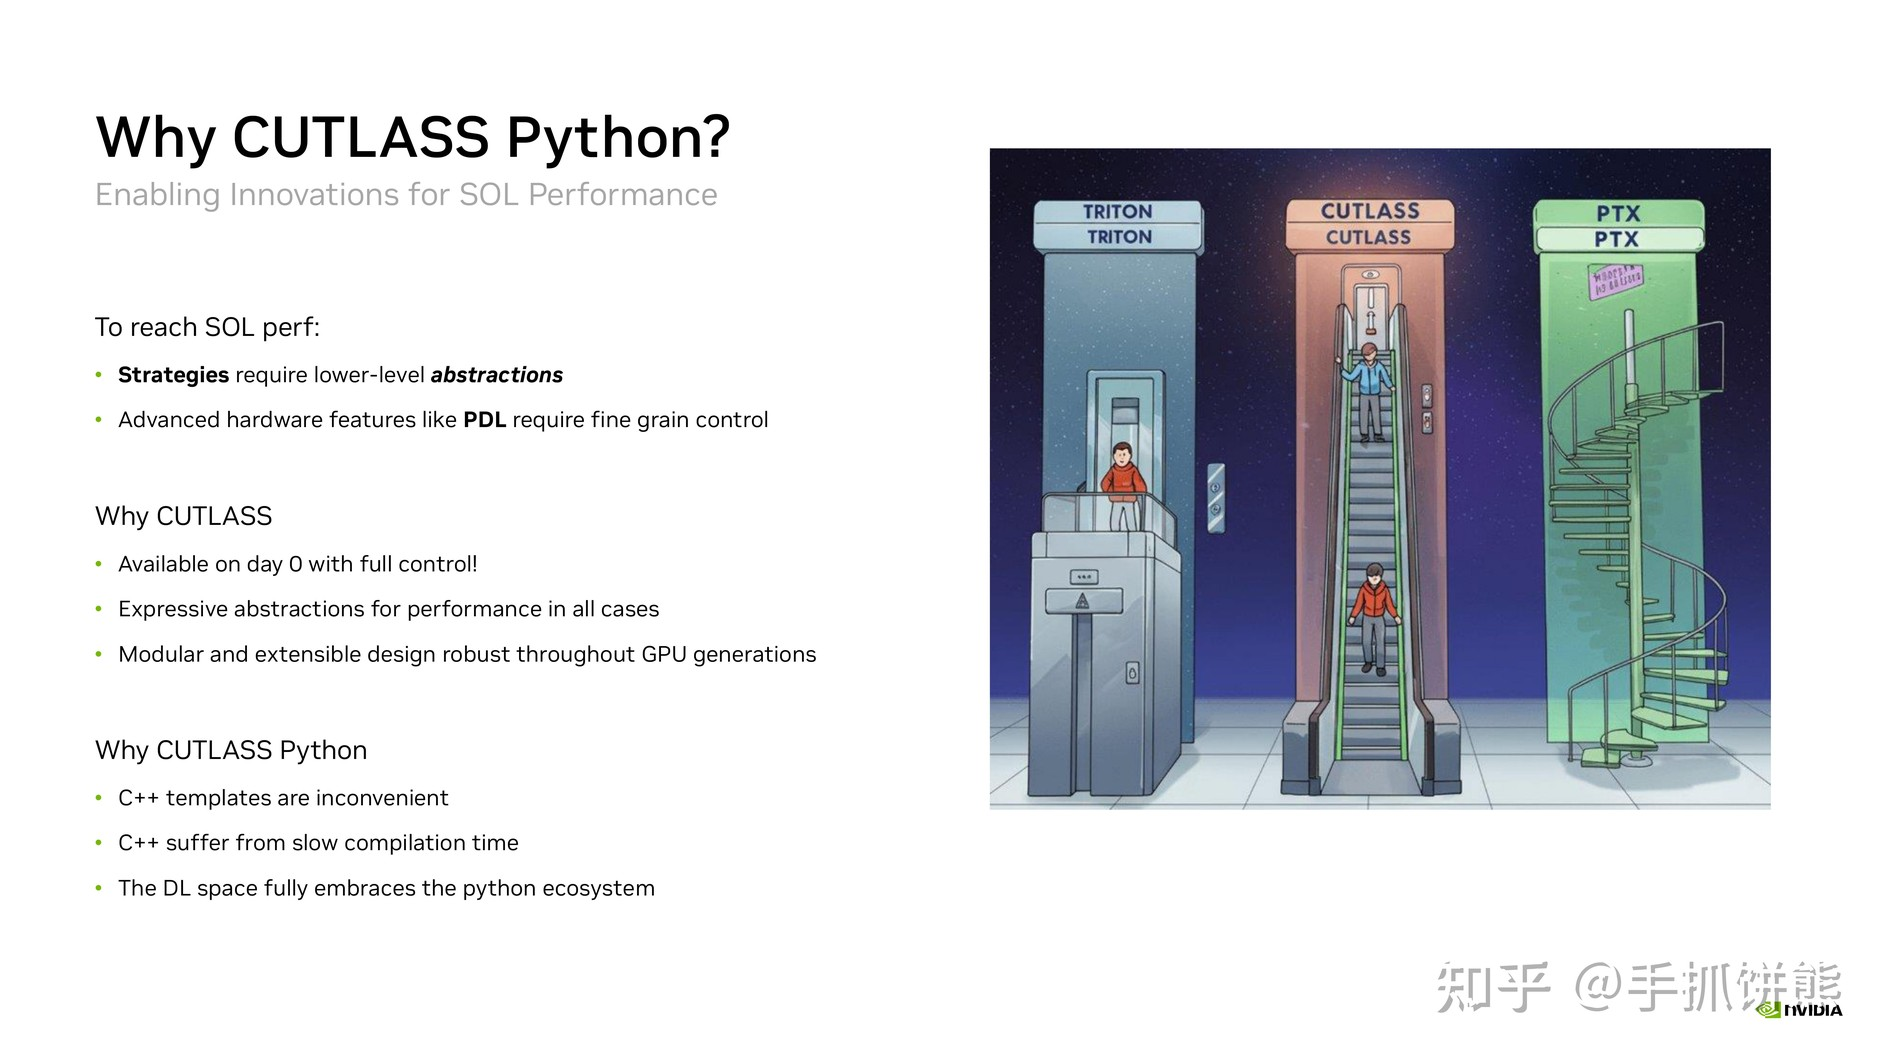
\includegraphics[width=0.9\textwidth]{figures/zhaoshangchun-03-cutlass-python/fig-01.jpg}
\end{figure}

\textbf{达到 SOL（Speed of Light）性能的挑战：}

要在现代 GPU 上达到 SOL 性能，开发者需要使用更低层级的抽象来精细控制硬件特性。特别是 Blackwell 架构引入的 \textbf{PDL（Programmatic Dependent Launch）} 等高级特性，需要细粒度的控制才能充分发挥其潜力。

\textbf{为什么选择 CUTLASS：}

\begin{itemize}
\item \textbf{Day-0 可用性：} CUTLASS 在新硬件发布的第一天即可使用，提供完全的硬件控制能力
\item \textbf{表达力强的抽象层：} 其抽象设计能够在各种场景下都获得高性能
\item \textbf{模块化和可扩展设计：} 历经多代 GPU 架构验证，设计稳健可靠
\end{itemize}

\textbf{为什么选择 Python 接口：}

\begin{itemize}
\item \textbf{C++ 模板编程不便：} CUTLASS C++ 的模板元编程对开发者极不友好，代码晦涩难懂
\item \textbf{编译时间过长：} C++ 模板会导致极长的编译时间，严重影响开发迭代效率
\item \textbf{Python 生态兼容：} 深度学习领域已全面拥抱 Python 生态系统，Python 接口能更好地融入现有工作流
\end{itemize}

\subsection{1.2 CUTLASS Python 的优势}

\begin{figure}[H]\centering
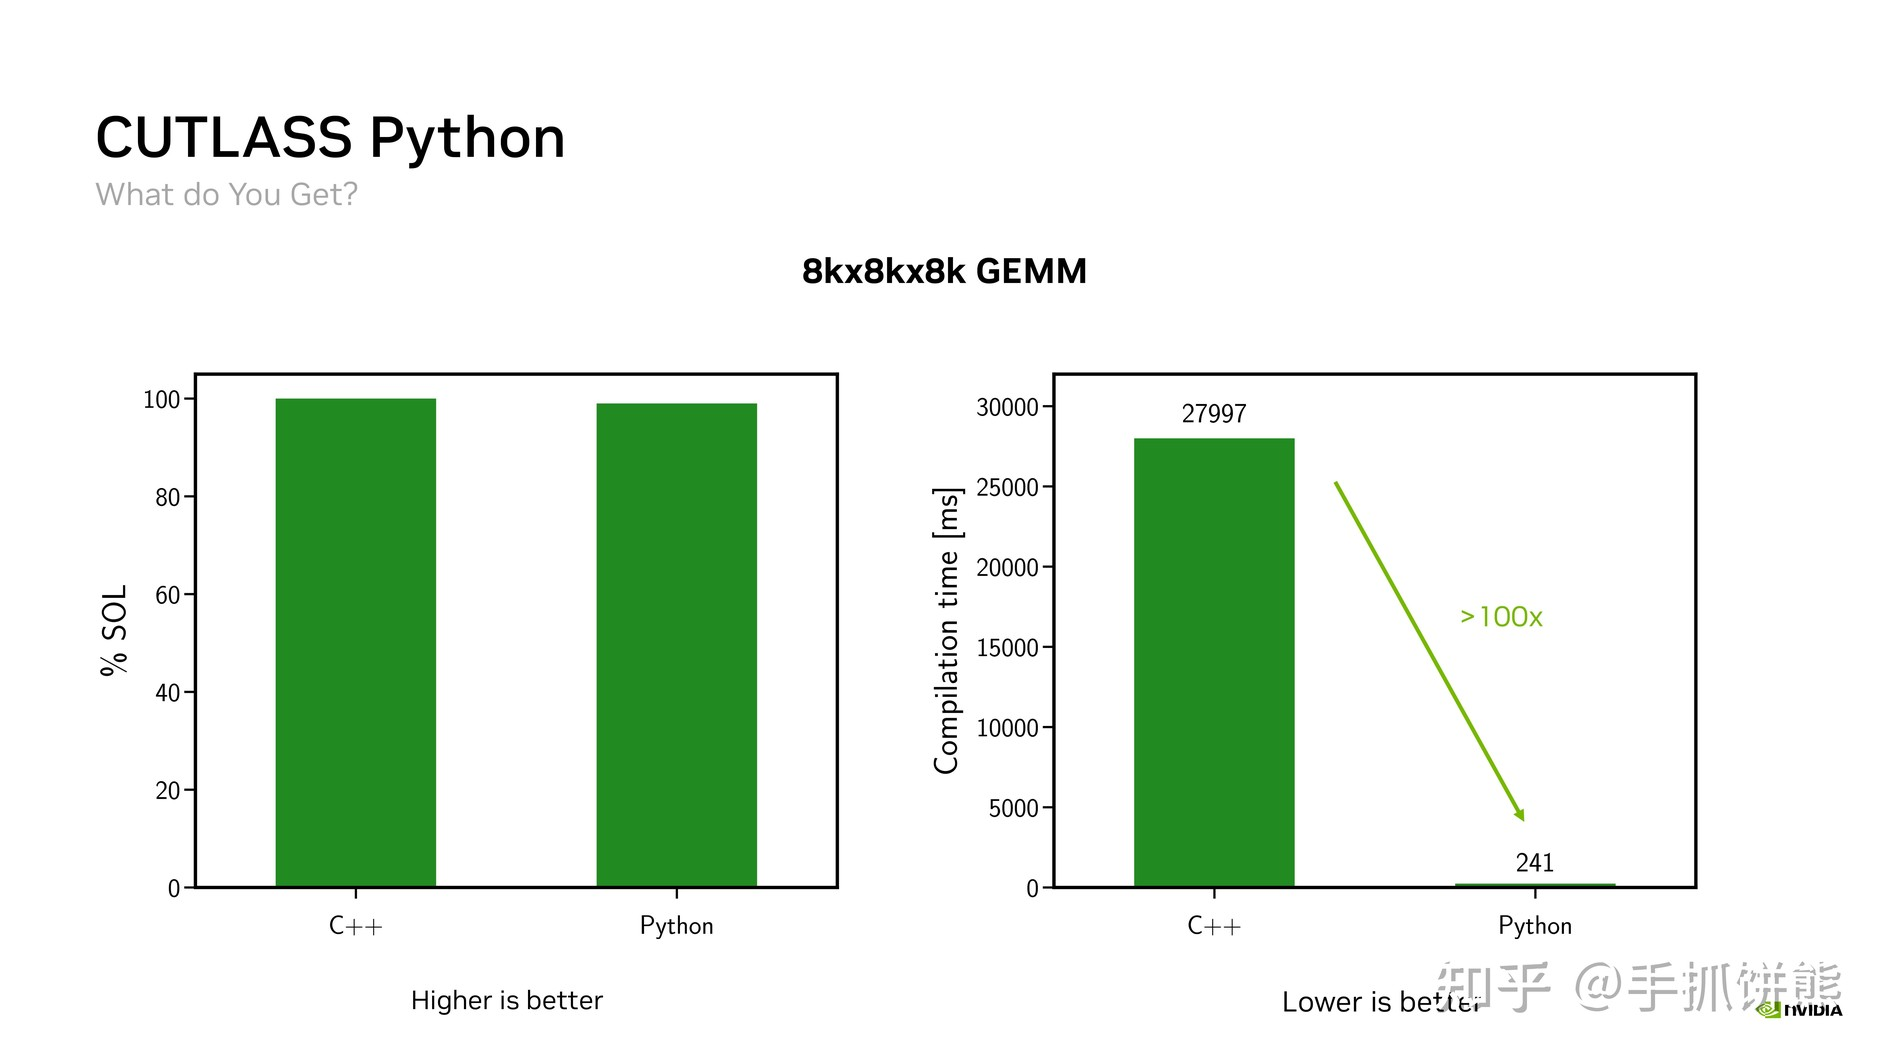
\includegraphics[width=0.9\textwidth]{figures/zhaoshangchun-03-cutlass-python/fig-02.jpg}
\end{figure}

\textbf{性能对比数据（8\allowbreak{}K×8\allowbreak{}K×8\allowbreak{}K GEMM）：}

CUTLASS Python 相较于传统方式实现了令人印象深刻的优势：

\begin{itemize}
\item \textbf{性能方面：} 在 8\allowbreak{}K×8\allowbreak{}K×8\allowbreak{}K GEMM 场景下达到了极高的 TFLOPS 吞吐量（图中 "Higher is better" 方向）
\item \textbf{编译速度：} 编译时间相较 C++ 实现缩短超过 \textbf{100 倍}（图中 "Lower is better" 方向）
\end{itemize}

这说明 CUTLASS Python 不仅没有牺牲运行时性能，还极大地改善了开发体验和迭代速度。JIT（Just-In-Time）编译和缓存机制使得 Python 接口在首次编译后可以达到与 C++ 相当的运行时性能。

\subsection{1.3 CUTLASS Python 架构概览}

\begin{figure}[H]\centering
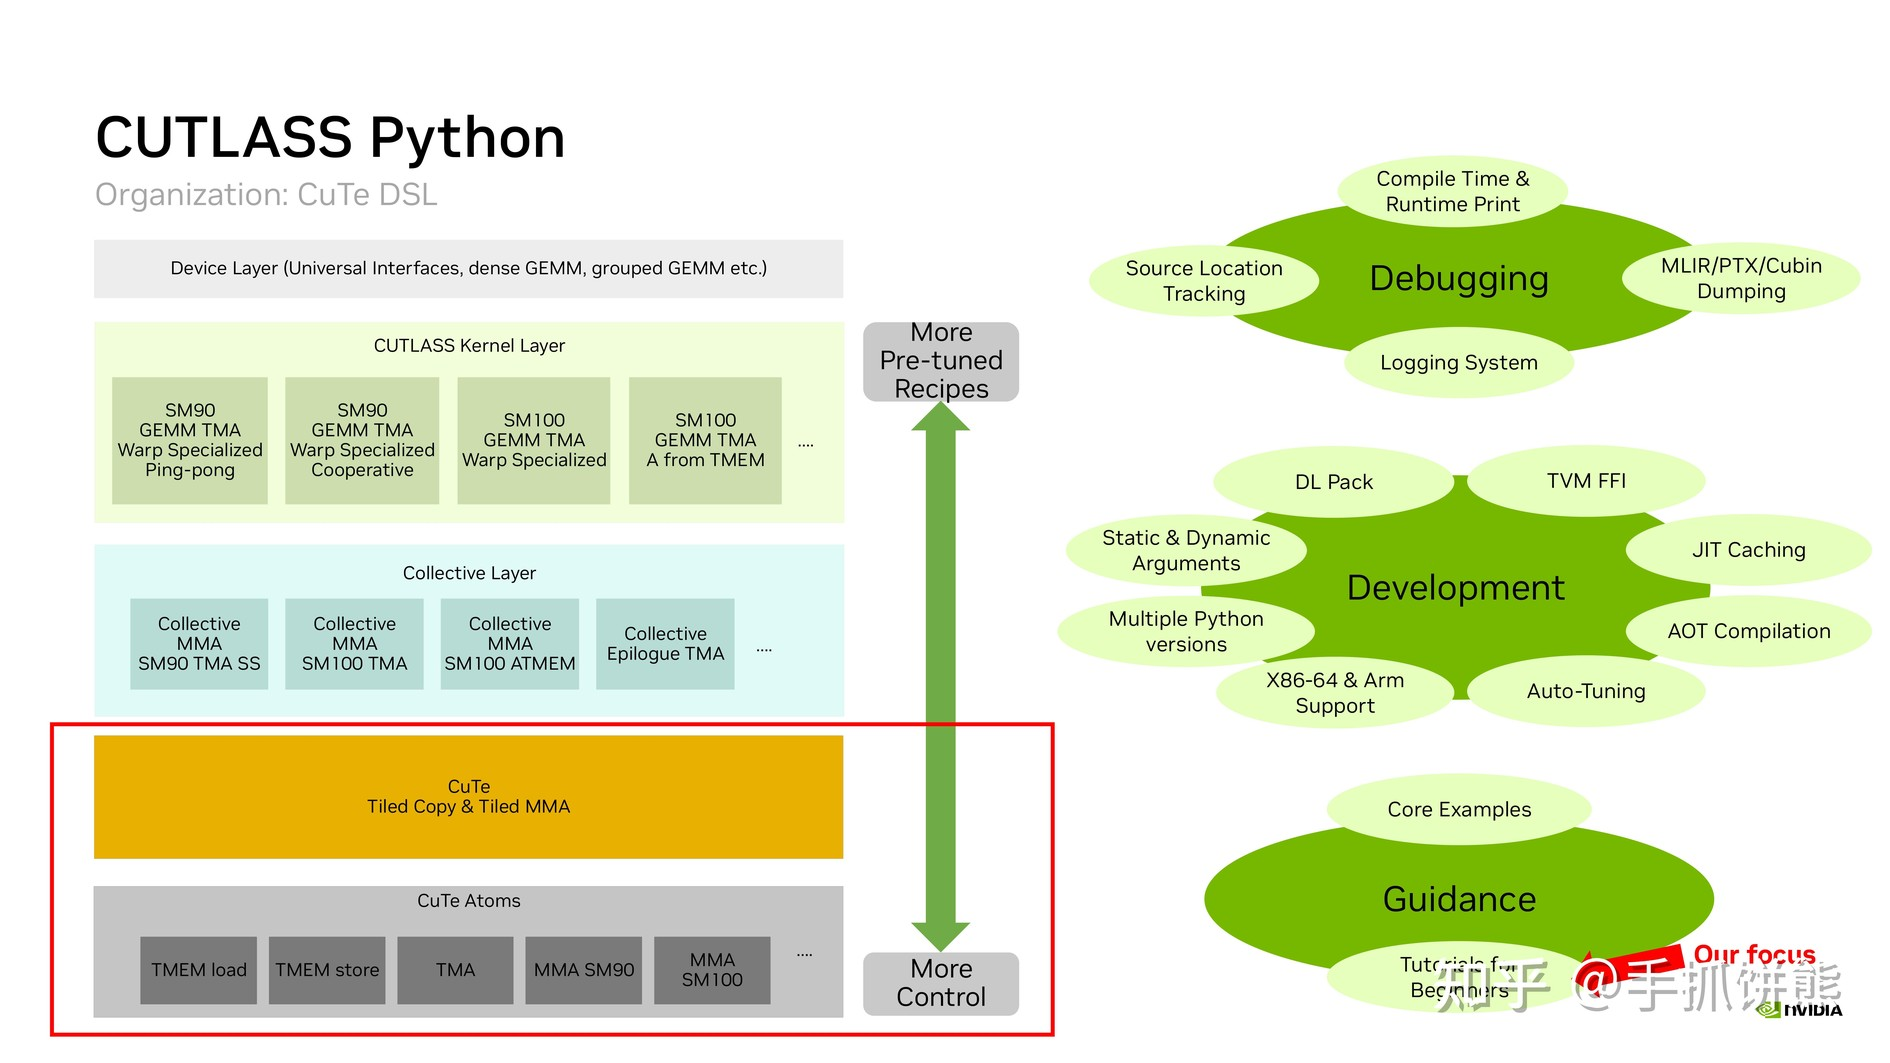
\includegraphics[width=0.9\textwidth]{figures/zhaoshangchun-03-cutlass-python/fig-03.jpg}
\end{figure}

\textbf{CUTLASS Python 的分层架构：}

CUTLASS Python 基于 \textbf{Cu\allowbreak{}Te DSL（Domain Specific Language）} 构建，形成了清晰的层次结构：

\textbf{底层 - Cu\allowbreak{}Te Atoms：}

\begin{itemize}
\item TMEM store/\allowbreak{}load（Tensor Memory 操作）
\item TMA（Tensor Memory Accelerator）
\item MMA SM90/\allowbreak{}SM100（Matrix Multiply-Accumulate 指令）
\end{itemize}

\textbf{中间层 - Tiled Copy \& Tiled MMA：}

\begin{itemize}
\item 提供分块拷贝和分块矩阵乘法的抽象
\item 支持不同架构的 Collective 操作（SM90 TMA SS、SM100 TMA、SM100 ATMEM 等）
\end{itemize}

\textbf{Collective Layer：}

\begin{itemize}
\item SM90 GEMM TMA Warp Specialized（Ping-pong/\allowbreak{}Cooperative 模式）
\item SM100 GEMM TMA Warp Specialized
\item SM100 GEMM TMA A from TMEM
\end{itemize}

\textbf{Device Layer（最高层）：}

\begin{itemize}
\item Universal Interfaces
\item Dense GEMM、Grouped GEMM 等
\end{itemize}

\textbf{开发生态支持：}

\begin{itemize}
\item \textbf{开发工具：} DL Pack、JIT Caching、TVM FFI、AOT Compilation、多 Python 版本支持、Auto-Tuning、静态/\allowbreak{}动态参数
\item \textbf{平台支持：} X86-64 \& Arm
\item \textbf{调试工具：} 编译时/\allowbreak{}运行时 Print、MLIR/\allowbreak{}PTX/\allowbreak{}Cubin Dumping、Source Location Tracking、Logging System
\item \textbf{指导资源：} Core Examples、Tutorials for Beginners
\end{itemize}

本演讲的重点聚焦在 \textbf{Tutorials for Beginners} 部分，帮助初学者从零开始理解 GEMM 优化。

\subsection{1.4 CUTLASS Python 生态现状}

\begin{figure}[H]\centering
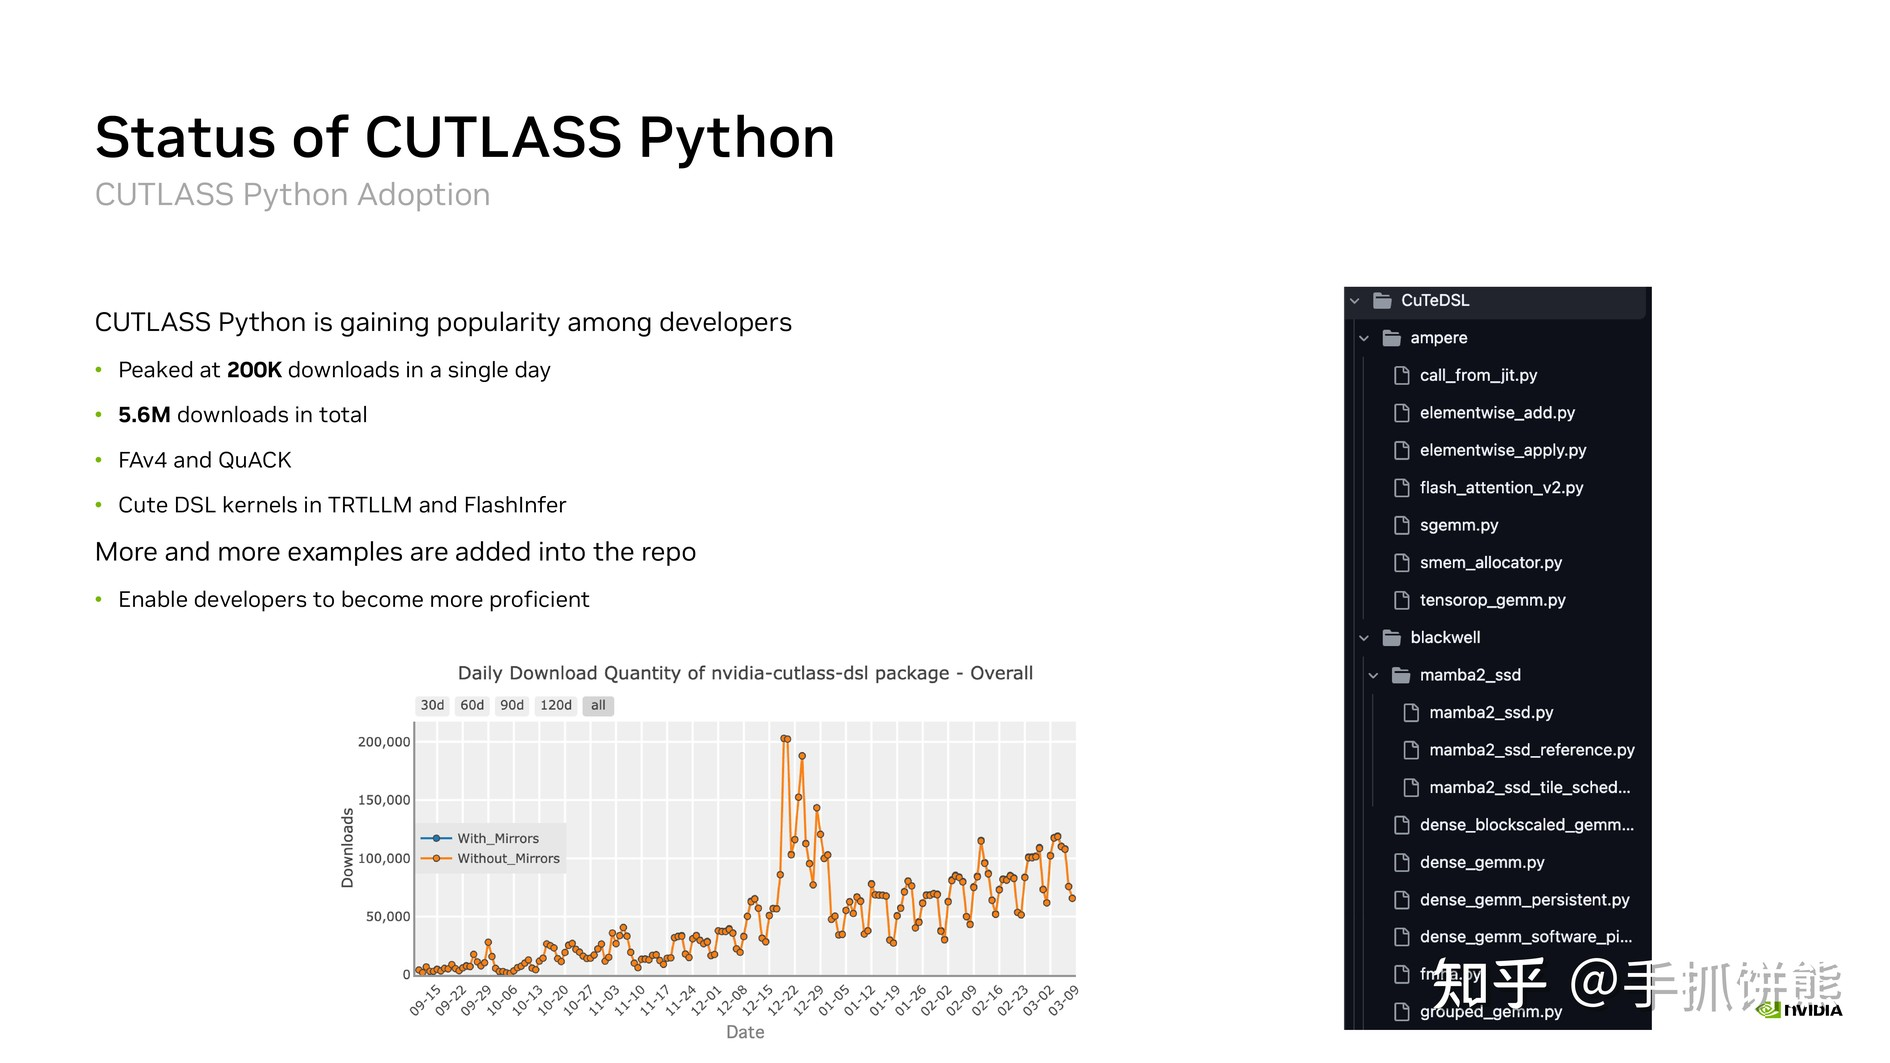
\includegraphics[width=0.9\textwidth]{figures/zhaoshangchun-03-cutlass-python/fig-04.jpg}
\end{figure}

\textbf{CUTLASS Python 的快速增长：}

\begin{itemize}
\item 单日下载峰值达 \textbf{200\allowbreak{}K 次}
\item 累计下载量达 \textbf{560 万次}
\item 已被多个知名项目采用：\textbf{FAv4}（Flash Attention v4）和 \textbf{Qu\allowbreak{}ACK}
\item Cu\allowbreak{}Te DSL 内核已集成到 \textbf{TRTLLM}（Tensor\allowbreak{}RT-LLM）和 \textbf{Flash\allowbreak{}Infer} 中
\end{itemize}

随着越来越多的示例被添加到代码仓库中，开发者能够更快速地上手和精通 CUTLASS Python 编程。

\subsection{1.5 Tutorial GEMM 的必要性}

\begin{figure}[H]\centering
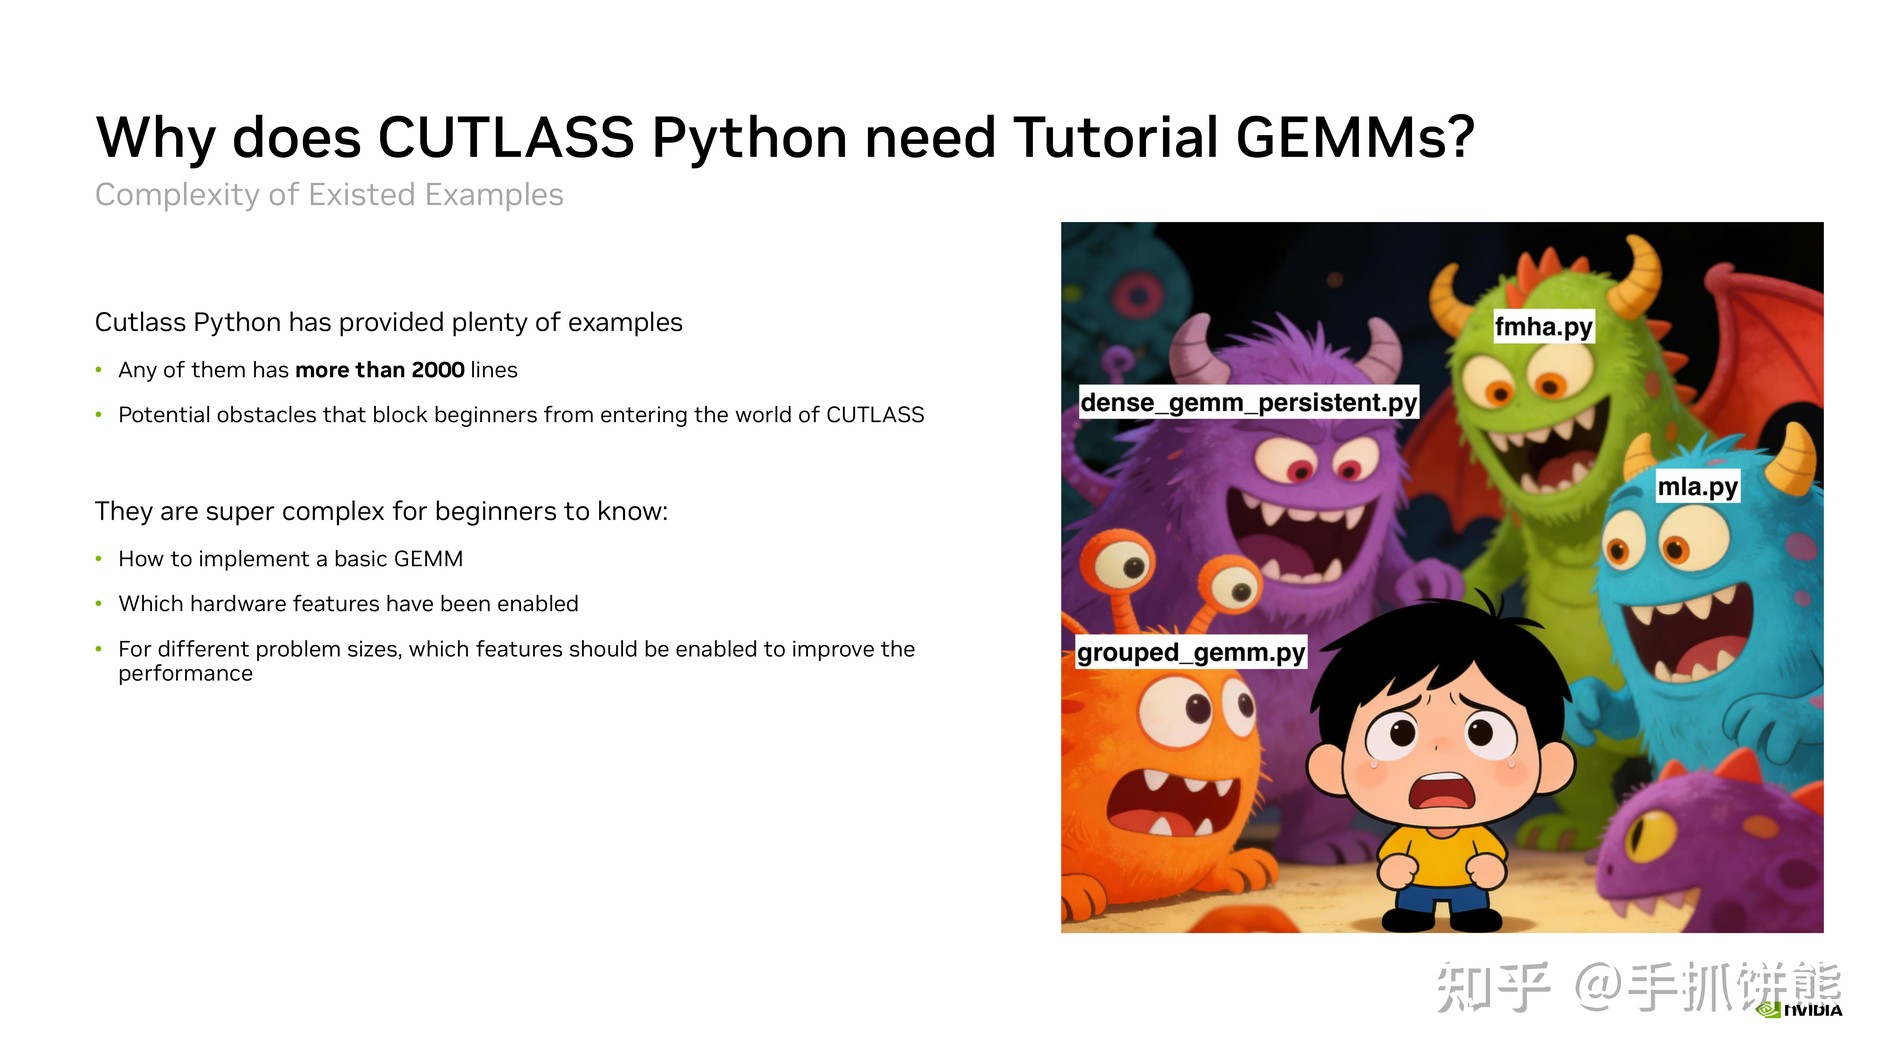
\includegraphics[width=0.9\textwidth]{figures/zhaoshangchun-03-cutlass-python/fig-05.jpg}
\end{figure}

\textbf{现有示例的复杂性问题：}

尽管 CUTLASS Python 提供了大量示例，但存在以下障碍：

\begin{itemize}
\item 每个示例都超过 \textbf{2000 行代码}，对初学者来说门槛过高
\item 初学者难以理解：
\item 如何实现一个基本的 GEMM
\item 哪些硬件特性已被启用
\item 对于不同问题规模，应该启用哪些特性来提升性能
\end{itemize}

这正是 \textbf{Tutorial GEMM} 系列的价值所在——提供循序渐进的学习路径。

\subsection{1.6 GEMM 的基本特性}

\begin{figure}[H]\centering
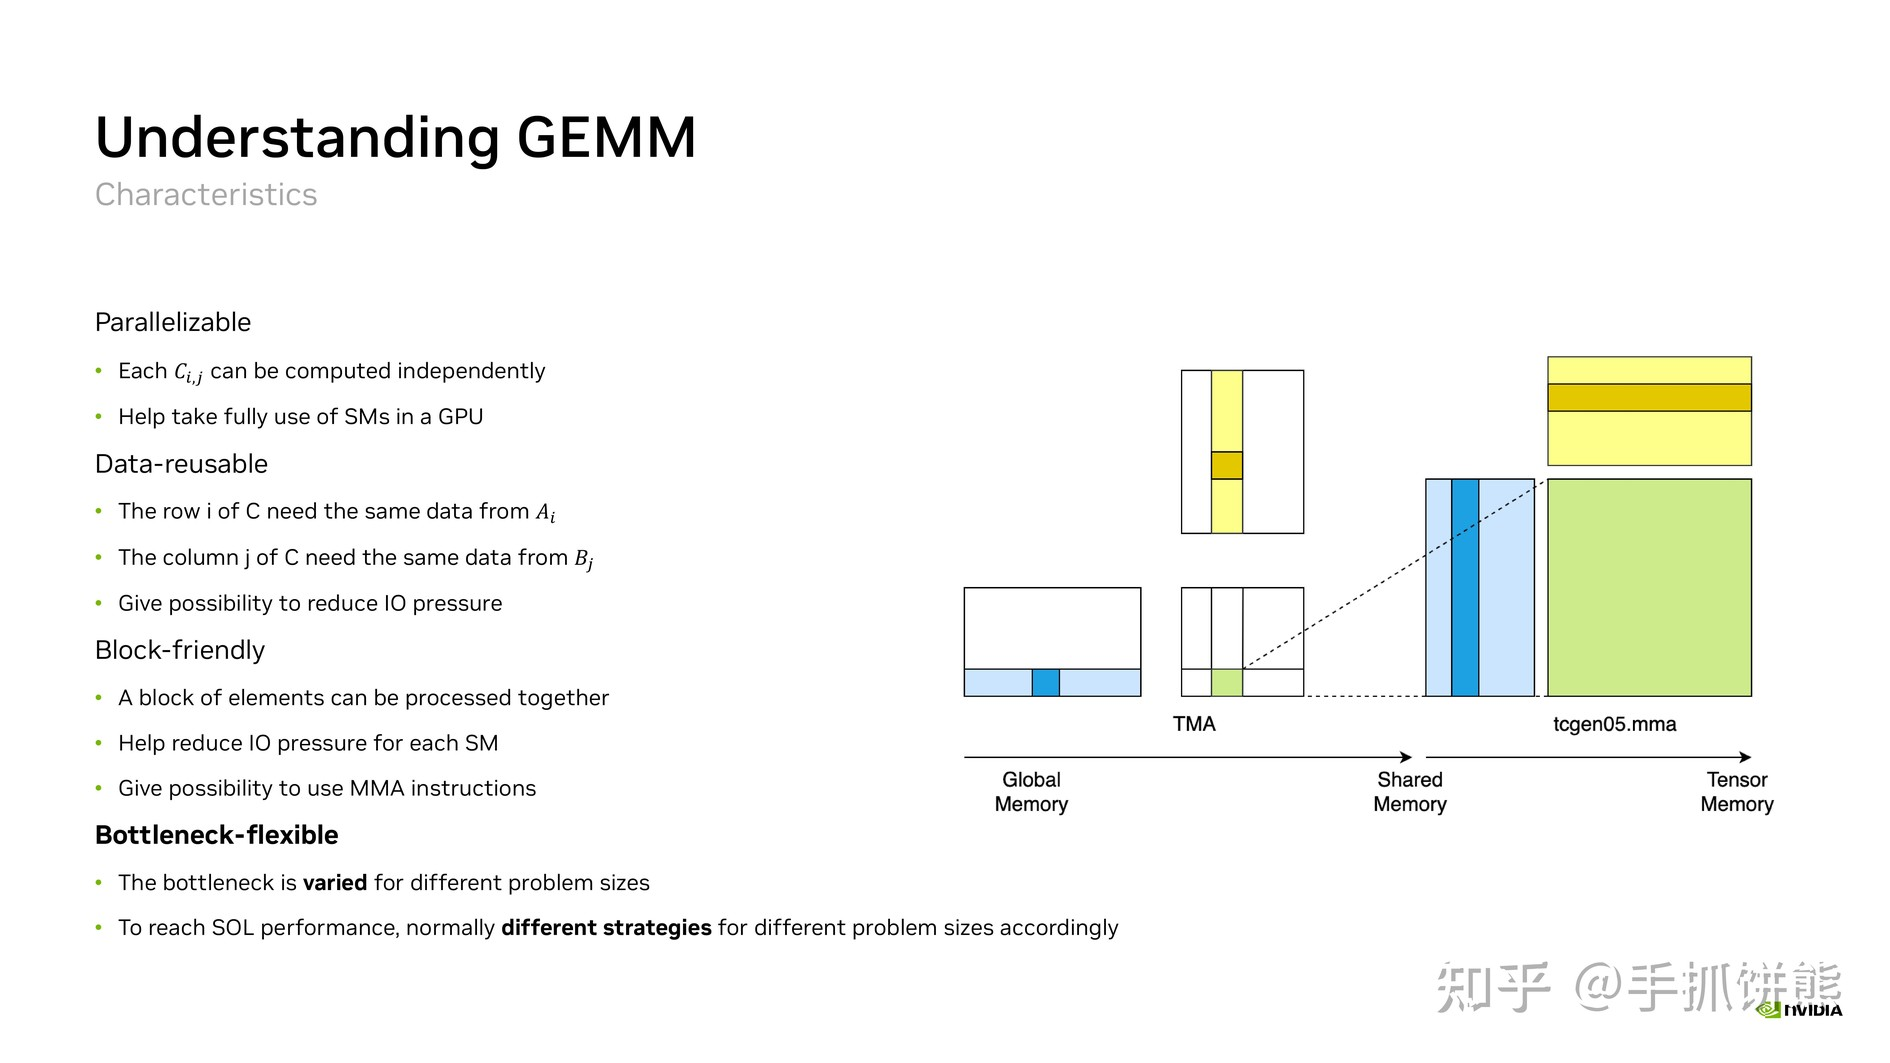
\includegraphics[width=0.9\textwidth]{figures/zhaoshangchun-03-cutlass-python/fig-06.jpg}
\end{figure}

\textbf{GEMM 的四大核心特性：}

\textbf{可并行性（Parallelizable）：}

\begin{itemize}
\item 输出矩阵 C 的每个元素 \$\$C\_\allowbreak{}\{i,j\$\$ 可以独立计算
\item 有助于充分利用 GPU 中的所有 SM（Streaming Multiprocessor）
\end{itemize}

\textbf{数据可复用性（Data-reusable）：}

\begin{itemize}
\item C 的第 i 行需要 A 矩阵的第 i 行 \$\$A\_\allowbreak{}\$\$ 的相同数据
\item C 的第 j 列需要 B 矩阵的第 j 列 \$\$B\_\allowbreak{}\$\$ 的相同数据
\item 这为减轻 IO 压力提供了可能性
\end{itemize}

\textbf{块友好性（Block-friendly）：}

\begin{itemize}
\item 一组元素可以被一起处理
\item 有助于减轻每个 SM 的 IO 压力
\item 为使用 MMA 指令提供了可能性
\end{itemize}

\textbf{瓶颈灵活性（Bottleneck-flexible）：}

\begin{itemize}
\item 不同问题规模下瓶颈各异
\item 要达到 SOL 性能，通常需要针对不同问题规模采用不同策略
\end{itemize}

\subsection{1.7 Tutorial GEMM 的贡献}

\begin{figure}[H]\centering
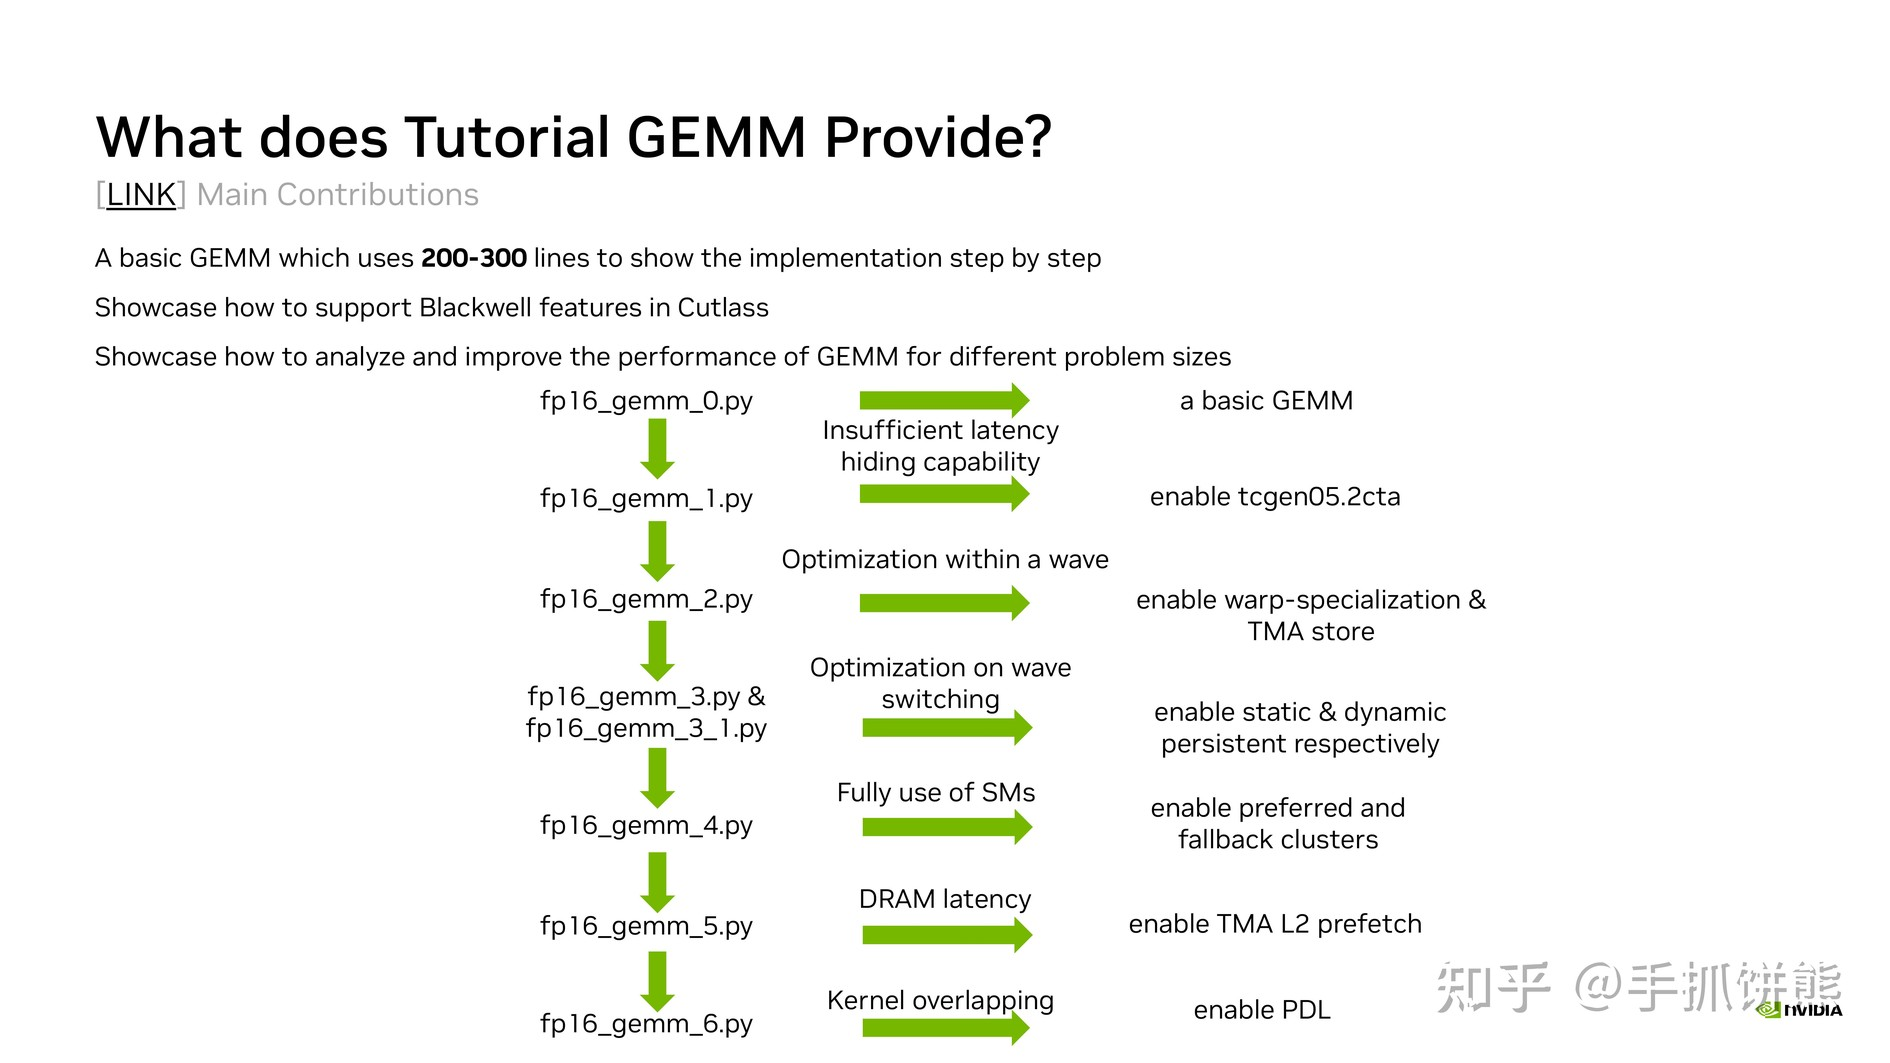
\includegraphics[width=0.9\textwidth]{figures/zhaoshangchun-03-cutlass-python/fig-07.jpg}
\end{figure}

\textbf{Tutorial GEMM 系列的主要贡献：}

提供了一系列渐进式优化的教程，每个仅需 200-300 行代码：

\begin{table}[htbp]\centering\small
\begin{adjustbox}{max width=\textwidth}
\begin{tabular}{lll}
\toprule
教程名称 & 优化技术 & 解决的问题 \\
\midrule
fp16gemm0.py & 基础 GEMM & 基线实现 \\
fp16gemm1.py & 启用 tcgen05.2cta & 延迟隐藏能力不足 \\
fp16gemm2.py & Warp Specialization + TMA Store & 波内优化 \\
fp16gemm3/\allowbreak{}3\_\allowbreak{}1.py & Static/\allowbreak{}Dynamic Persistent & 波间切换优化 \\
fp16gemm4.py & Preferred/\allowbreak{}Fallback Clusters & 充分利用 SM \\
fp16gemm5.py & PDL & 内核重叠 \\
fp16gemm6.py & TMA L2 Prefetch & DRAM 延迟 \\
\bottomrule
\end{tabular}
\end{adjustbox}
\end{table}

\section{第二章：基础 GEMM 概览}

本章详细解析基础 GEMM（Tutorial 0）的实现原理，这是所有后续优化的基础。

\subsection{2.1 基础 GEMM 工作流程}

\begin{figure}[H]\centering
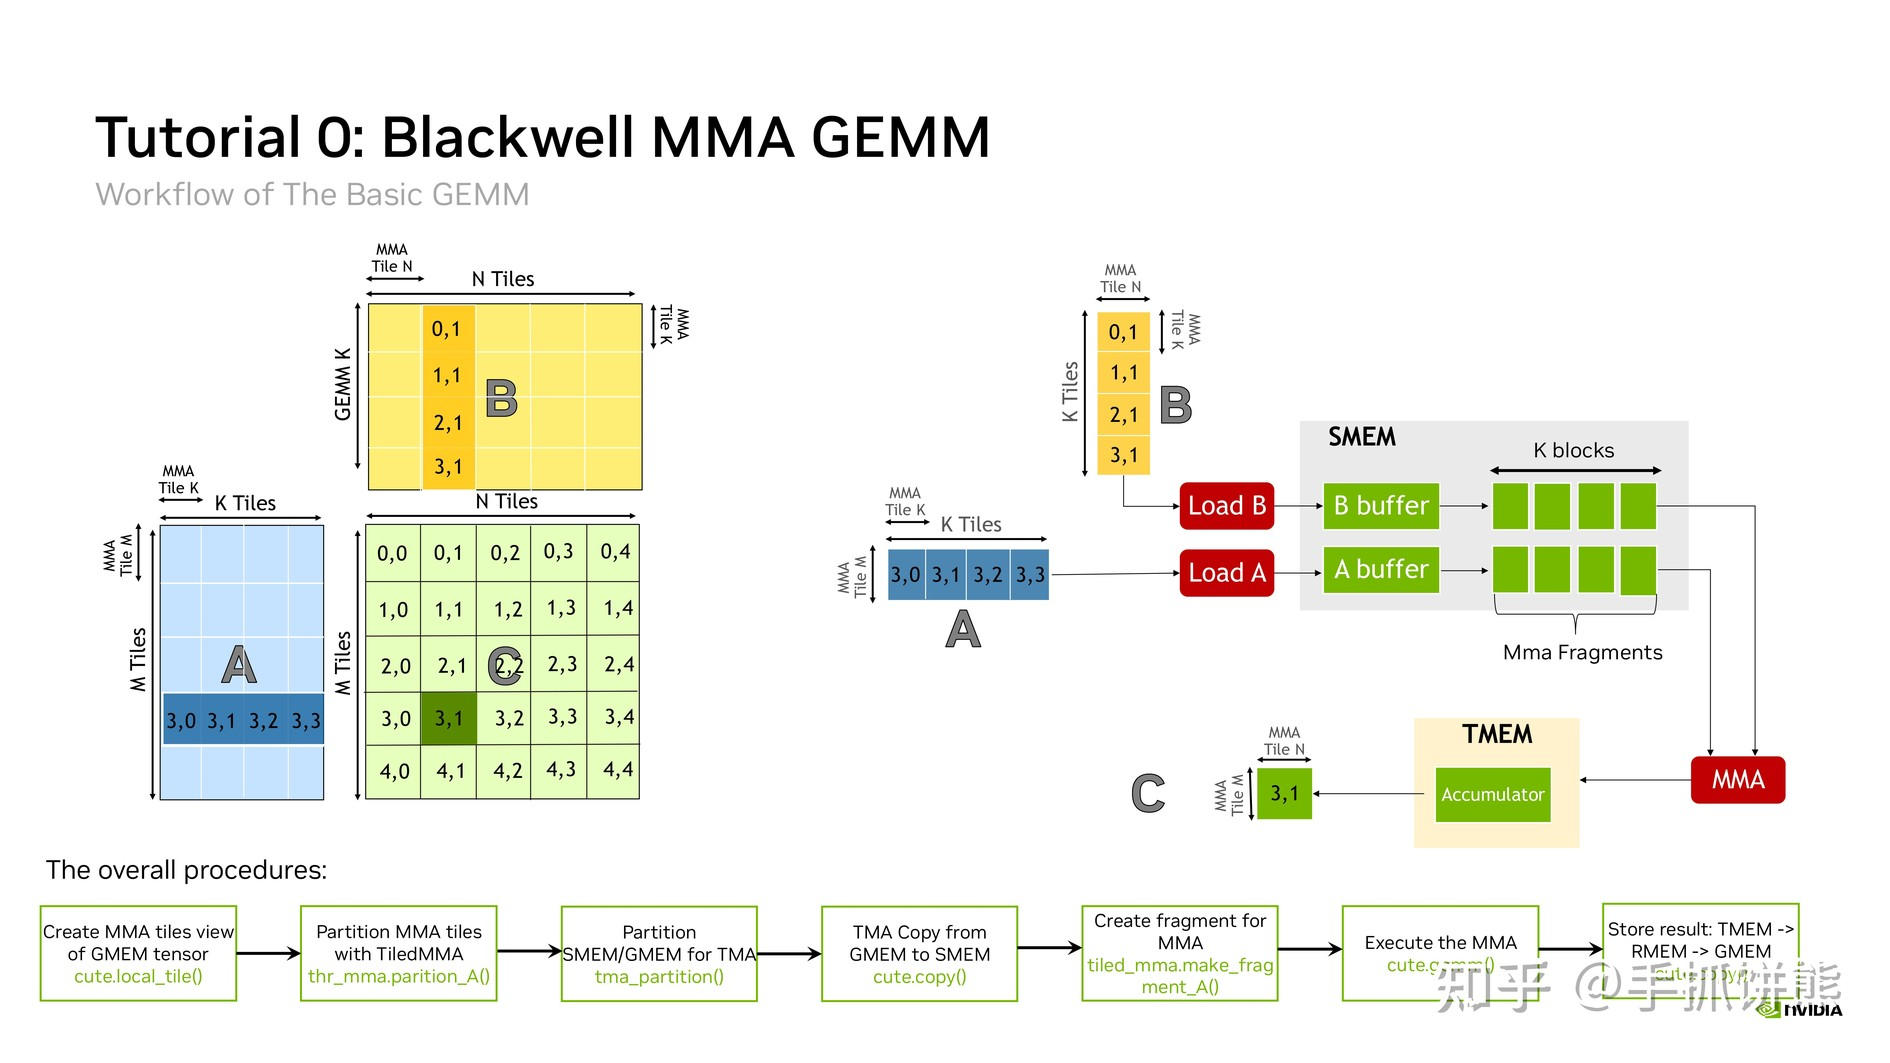
\includegraphics[width=0.9\textwidth]{figures/zhaoshangchun-03-cutlass-python/fig-08.jpg}
\end{figure}

\textbf{整体计算流程：}

基础 GEMM 的工作流程分为以下关键步骤：

\textbf{Step 1 - 创建 MMA Tile 视图（\texttt{cute.\allowbreak{}local\_\allowbreak{}tile()}）：}

将全局内存（GMEM）中的大矩阵按照 MMA Tile 大小进行分块。在图中可以看到，矩阵 C 被划分为 M Tiles × N Tiles 的网格，每个 CTA 负责计算其中一个 tile（如图中标注的 C[3,1]）。对应的 A 矩阵取出相应的行 tile，B 矩阵取出相应的列 tile。

\textbf{Step 2 - 使用 Tiled\allowbreak{}MMA 分区（\texttt{thr\_\allowbreak{}mma.\allowbreak{}partition\_\allowbreak{}A()}）：}

将 MMA Tile 进一步分配给具体的线程。Tiled\allowbreak{}MMA 抽象定义了线程如何协作完成矩阵乘法运算，每个线程负责 tile 中的特定元素子集。

\textbf{Step 3 - 为 TMA 分区 SMEM/\allowbreak{}GMEM（\texttt{tma\_\allowbreak{}partition()}）：}

Tensor Memory Accelerator（TMA）是 Blackwell 架构的硬件加速器，负责高效地在全局内存和共享内存之间传输数据。这一步为 TMA 操作准备好源和目标的内存分区。

\textbf{Step 4 - TMA 从 GMEM 拷贝到 SMEM（\texttt{cute.\allowbreak{}copy()}）：}

使用 TMA 硬件单元将数据从全局内存异步加载到共享内存（SMEM）。图中的 "A buffer" 和 "B buffer" 即为 SMEM 中的缓冲区。通过多缓冲（multi-buffering）策略，可以在计算一个 K block 的同时加载下一个 K block 的数据。

\textbf{Step 5 - 创建 MMA Fragment（\texttt{t\allowbreak{}i\allowbreak{}l\allowbreak{}e\allowbreak{}d\allowbreak{}\_\allowbreak{}m\allowbreak{}m\allowbreak{}a\allowbreak{}.\allowbreak{}m\allowbreak{}a\allowbreak{}k\allowbreak{}e\allowbreak{}\_\allowbreak{}f\allowbreak{}r\allowbreak{}a\allowbreak{}g\allowbreak{}m\allowbreak{}e\allowbreak{}n\allowbreak{}t\allowbreak{}\_\allowbreak{}A\allowbreak{}(\allowbreak{})}）：}

从 SMEM 中创建 MMA 操作所需的数据片段（fragment）。在 Blackwell 架构中，这些片段存储在 TMEM（Tensor Memory）中，这是一种专为 Tensor Core 优化的内存层级。

\textbf{Step 6 - 执行 MMA（\texttt{cute.\allowbreak{}gemm()}）：}

调用 Tensor Core 执行矩阵乘累加运算。结果存储在 TMEM 中的累加器（Accumulator）里。整个 K 维度的循环通过 "K blocks" 迭代，每次处理一个 MMA Tile K 大小的数据。

\textbf{Step 7 - 存储结果：TMEM → RMEM → GMEM（\texttt{cute.\allowbreak{}copy()}）：}

将最终计算结果从 TMEM 传输到寄存器（RMEM），再从寄存器写回全局内存。这是基础版本中最简单的 epilogue 实现。

\subsection{2.2 数据分块与内存层次（续）}

\begin{figure}[H]\centering
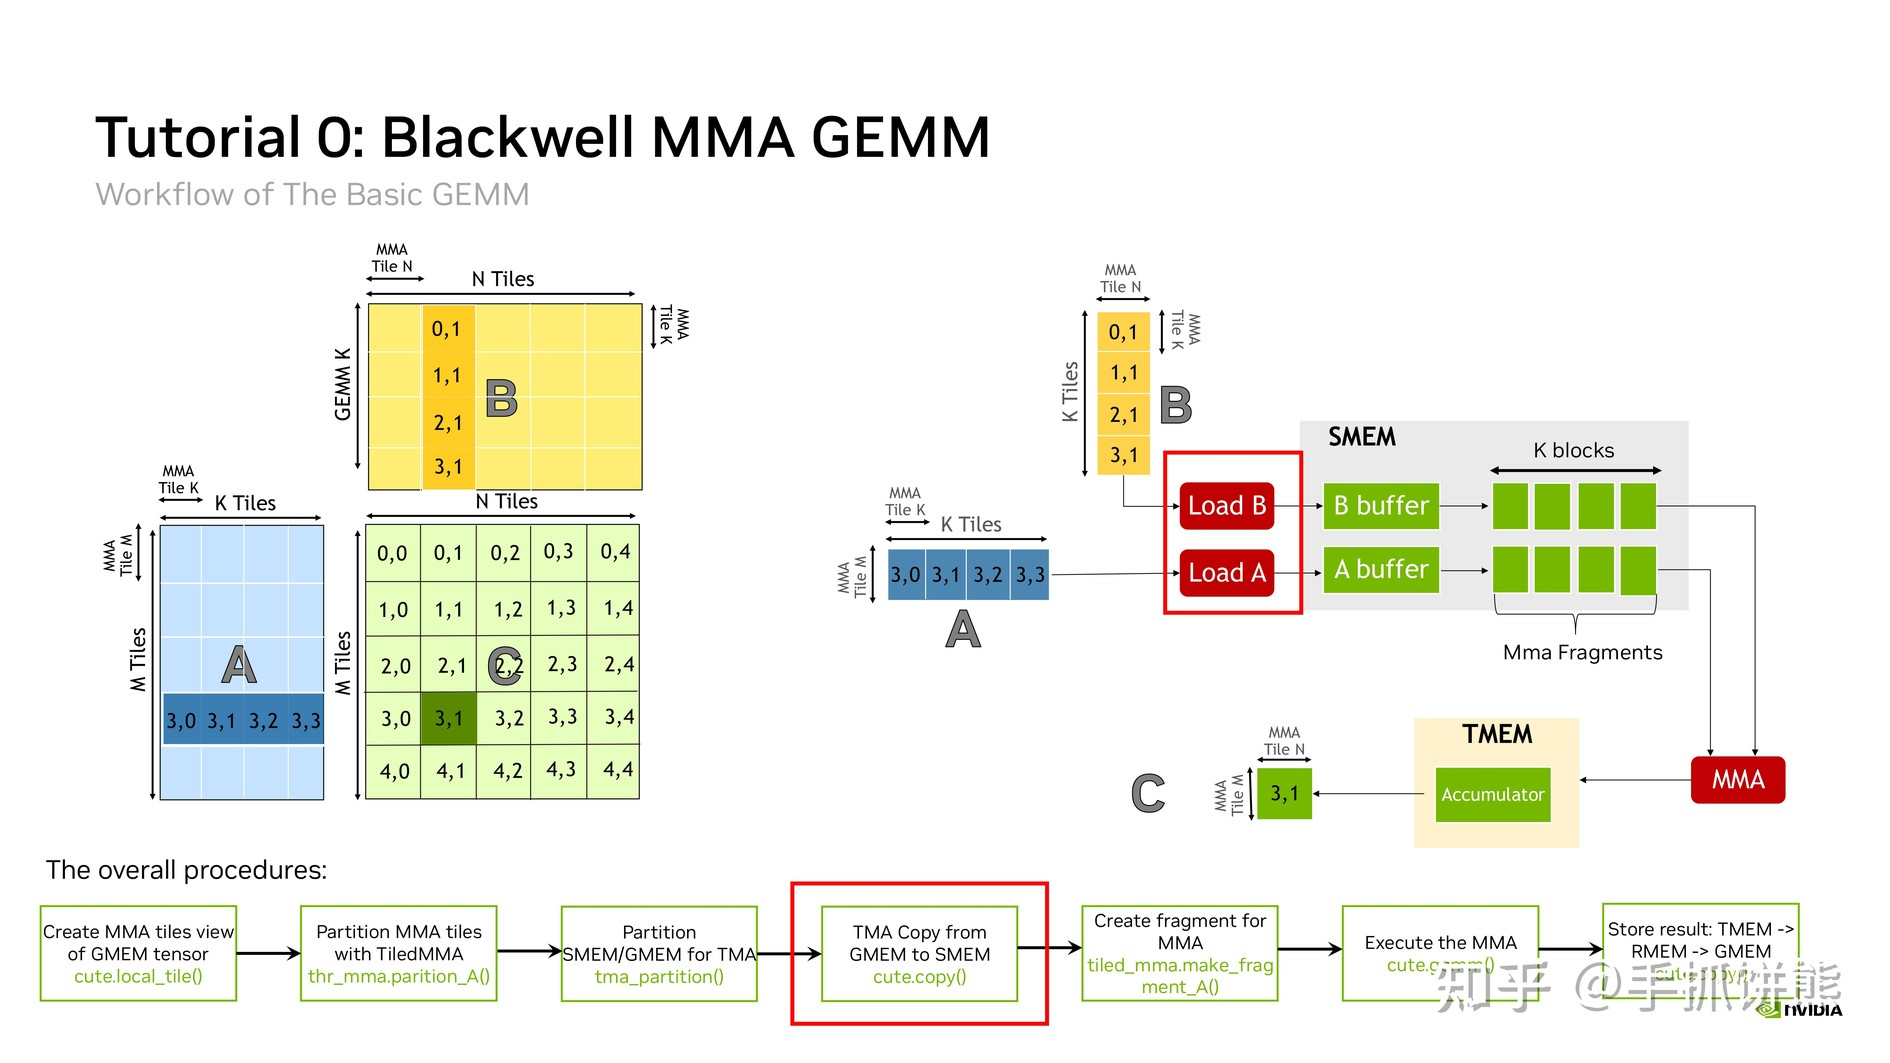
\includegraphics[width=0.9\textwidth]{figures/zhaoshangchun-03-cutlass-python/fig-09.jpg}
\end{figure}

\textbf{分块策略的详细说明：}

图中展示了数据如何在不同内存层次间流动：

\begin{itemize}
\item \textbf{GMEM → SMEM：} 通过 TMA 将 A 和 B 矩阵的 tile 加载到 SMEM 的 buffer 中
\item \textbf{SMEM → TMEM/\allowbreak{}RMEM：} 通过 MMA Fragment 的创建过程，数据被送入 Tensor Core 的输入缓冲
\item \textbf{TMEM → GMEM：} 计算完成后将累加器结果写回全局内存
\end{itemize}

关键的 tiling 参数：

\begin{itemize}
\item \textbf{MMA Tile M/\allowbreak{}N/\allowbreak{}K：} 定义了 Tensor Core 单次 MMA 操作的大小
\item \textbf{K Tiles：} 沿 K 维度的分块数量，决定了主循环的迭代次数
\item \textbf{ab\_\allowbreak{}stages：} SMEM 中的缓冲区数量，决定了 software pipeline 的深度
\end{itemize}

\subsection{2.3 基础 GEMM 性能基线}

\begin{figure}[H]\centering
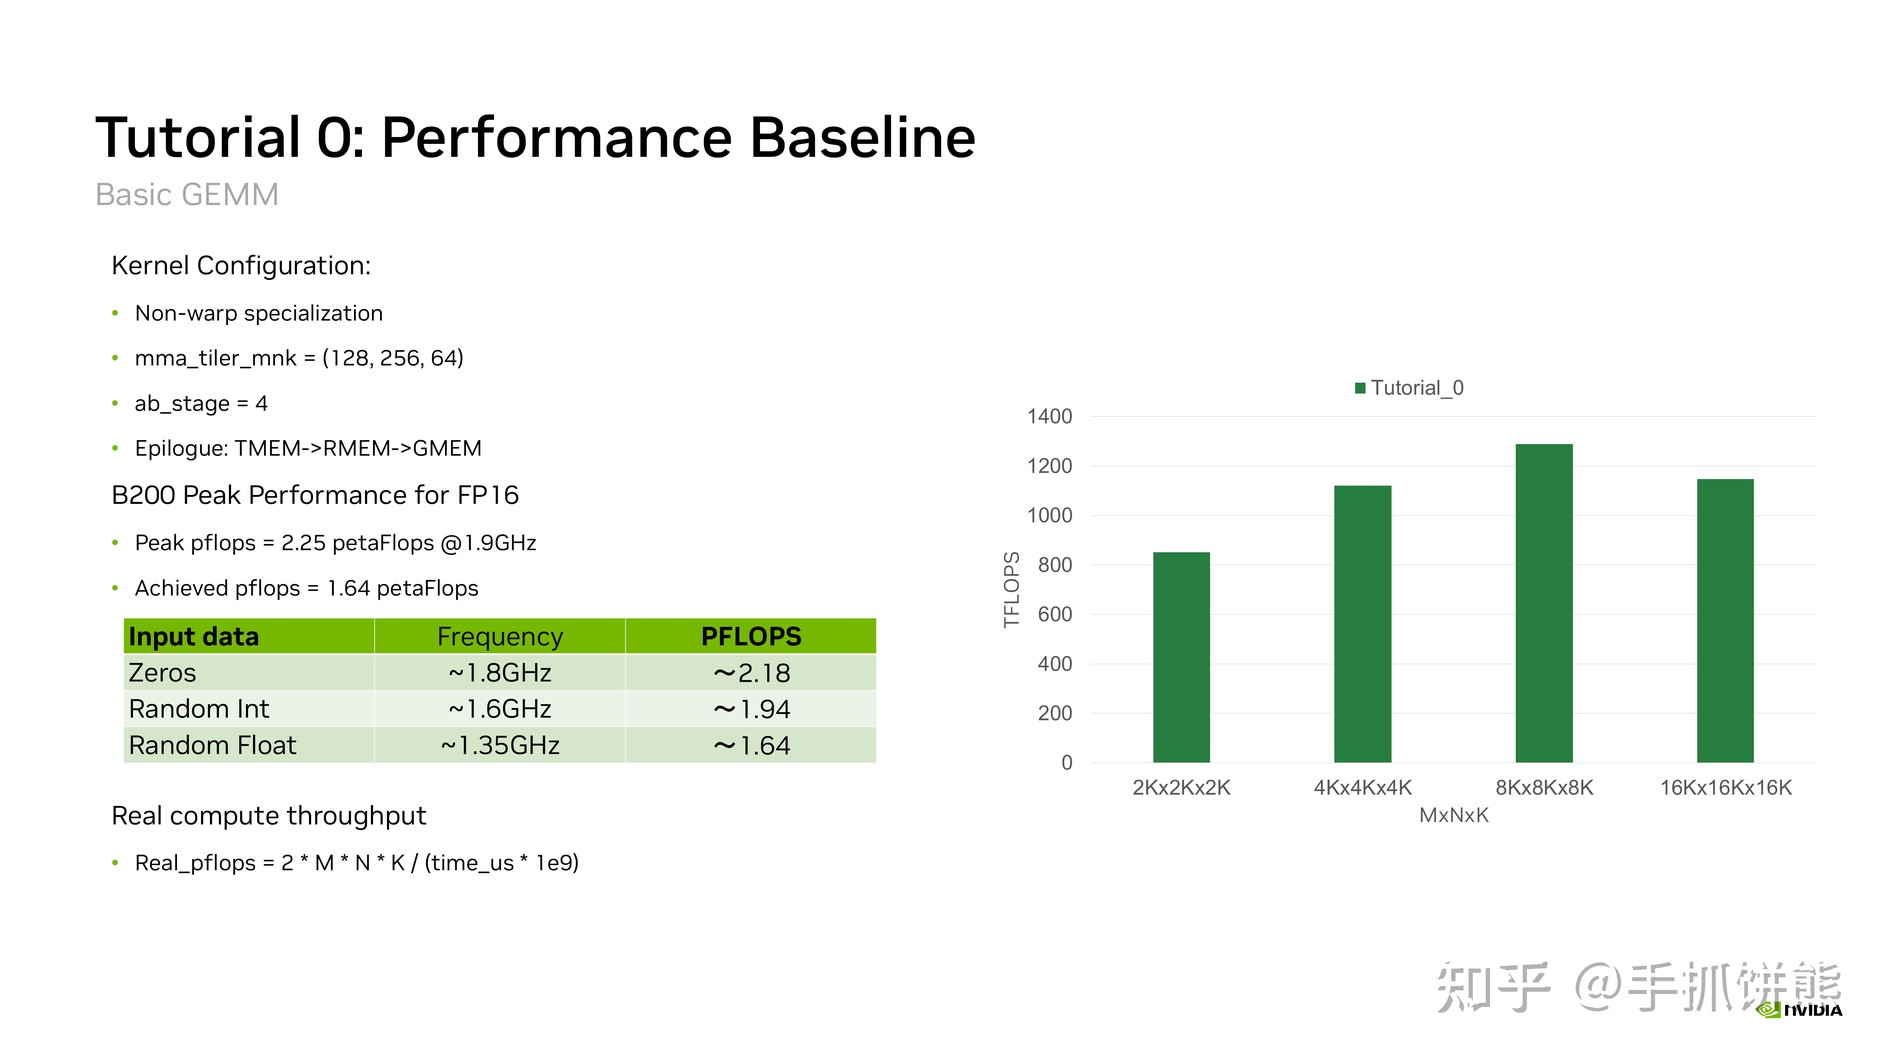
\includegraphics[width=0.9\textwidth]{figures/zhaoshangchun-03-cutlass-python/fig-10.jpg}
\end{figure}

\textbf{内核配置：}

\begin{itemize}
\item 非 Warp Specialization 模式
\item MMA tiler 大小：128×256×64（M×N×K）
\item ab\_\allowbreak{}stages = 4（SMEM 缓冲区数量）
\item Epilogue：TMEM → RMEM → GMEM（最基本的写回方式）
\end{itemize}

\textbf{B200 FP16 峰值性能分析：}

B200 GPU 的理论峰值性能为 \textbf{2.25 peta\allowbreak{}FLOPS}（@ 1.9\allowbreak{}GHz），但实际可达峰值取决于输入数据类型：

\begin{table}[htbp]\centering\small
\begin{adjustbox}{max width=\textwidth}
\begin{tabular}{lll}
\toprule
输入数据 & 频率 & PFLOPS \\
\midrule
Zeros（全零） & \textasciitilde{}1.8 GHz & \textasciitilde{}2.18 \\
Random Int（随机整数） & \textasciitilde{}1.6 GHz & \textasciitilde{}1.94 \\
Random Float（随机浮点） & \textasciitilde{}1.35 GHz & \textasciitilde{}1.64 \\
\bottomrule
\end{tabular}
\end{adjustbox}
\end{table}

这是因为 GPU 的 DVFS（Dynamic Voltage and Frequency Scaling）机制会根据功耗和温度动态调整频率。随机浮点数据的功耗最大，因此频率最低。

\textbf{性能数据：}

从图表来看，Tutorial 0 在不同问题规模下的性能：

\begin{itemize}
\item 2\allowbreak{}K×2\allowbreak{}K×2\allowbreak{}K：相对较低，受 kernel launch 开销影响
\item 4\allowbreak{}K×4\allowbreak{}K×4\allowbreak{}K：逐步提升
\item 8\allowbreak{}K×8\allowbreak{}K×8\allowbreak{}K：约 1200+ TFLOPS
\item 16\allowbreak{}K×16\allowbreak{}K×16\allowbreak{}K：约 1300+ TFLOPS
\end{itemize}

基线性能为 \textbf{1.64 peta\allowbreak{}FLOPS（1640 TFLOPS）}，这为后续优化提供了起点。

\section{第三章：渐进式 GEMM 优化——计算密集型场景}

本章是整个演讲的核心部分，详细展示了如何从基线性能逐步优化到接近理论峰值。

\subsection{3.1 优化路径总览}

\begin{figure}[H]\centering
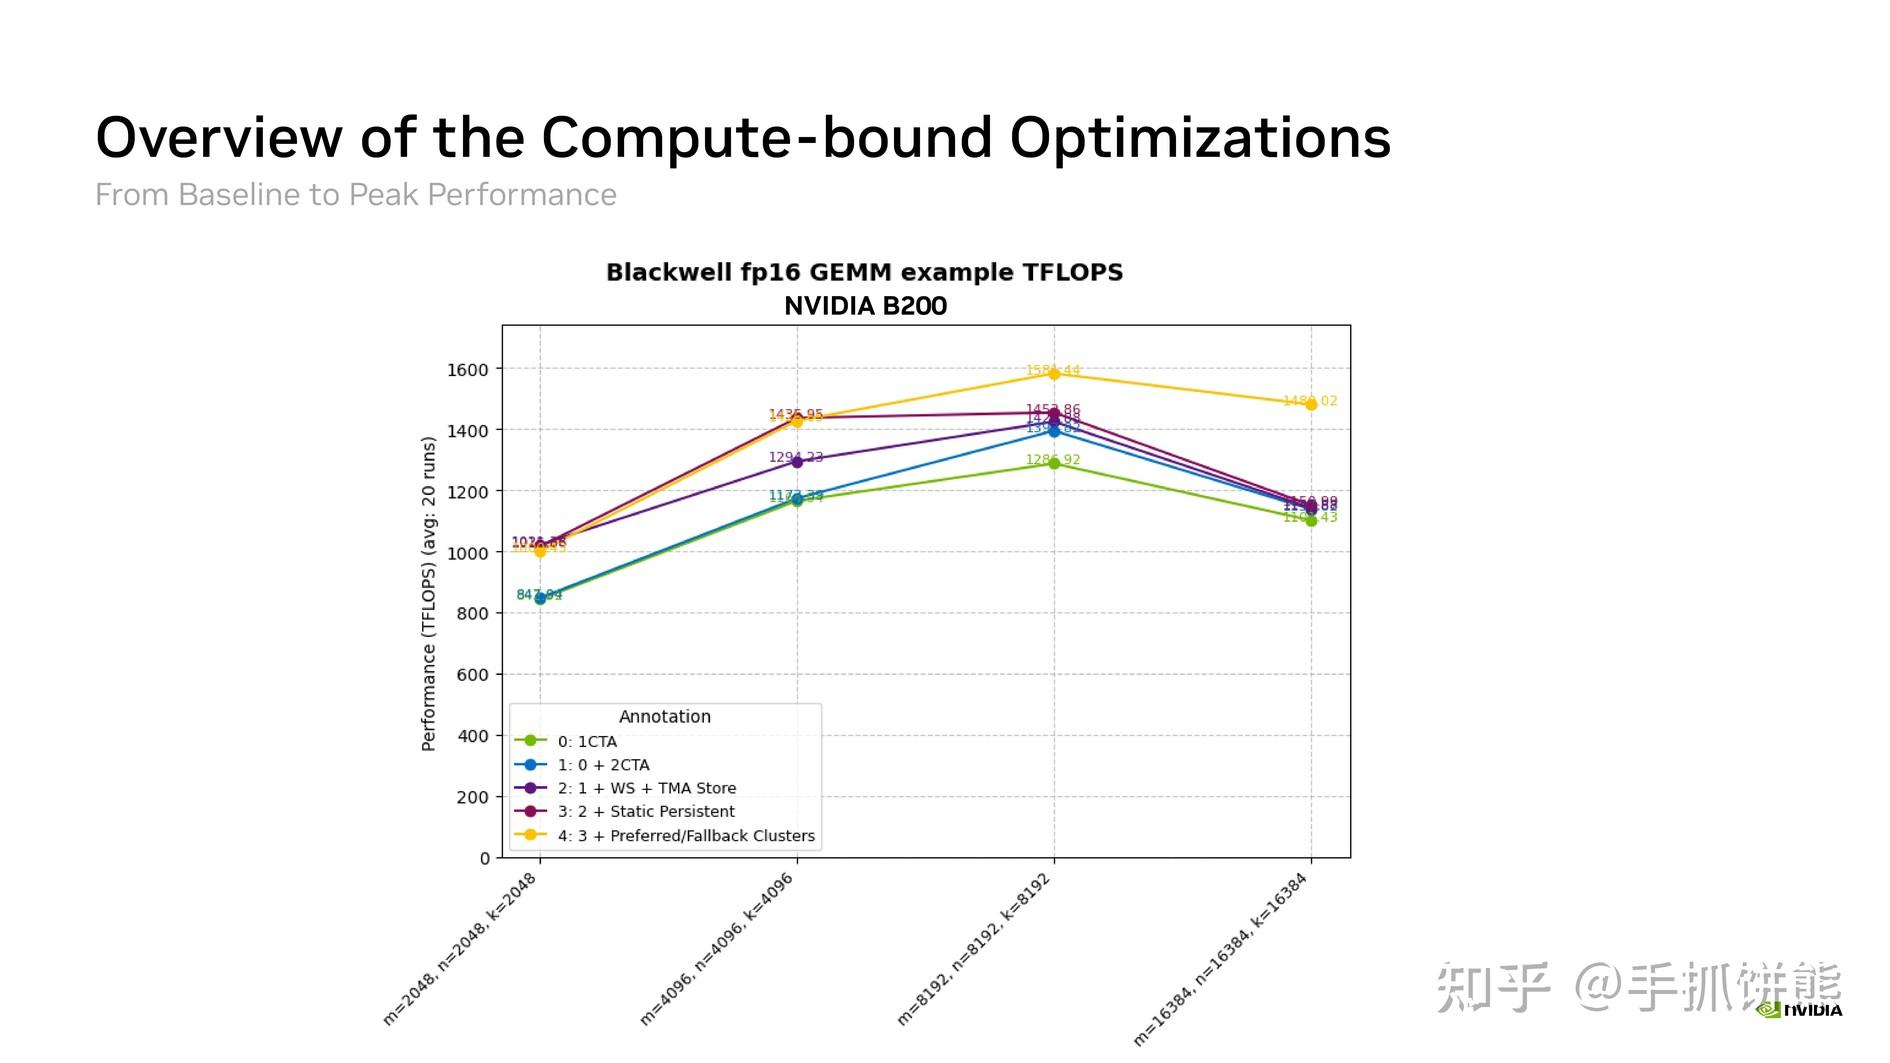
\includegraphics[width=0.9\textwidth]{figures/zhaoshangchun-03-cutlass-python/fig-11.jpg}
\end{figure}

该图展示了从基线到峰值性能的完整优化路径，每一步优化都叠加在前一步之上，最终在 NVIDIA B200 上达到接近 SOL 的性能。

\subsection{3.2 Tutorial 0：Software Pipeline 与延迟隐藏}

\begin{figure}[H]\centering
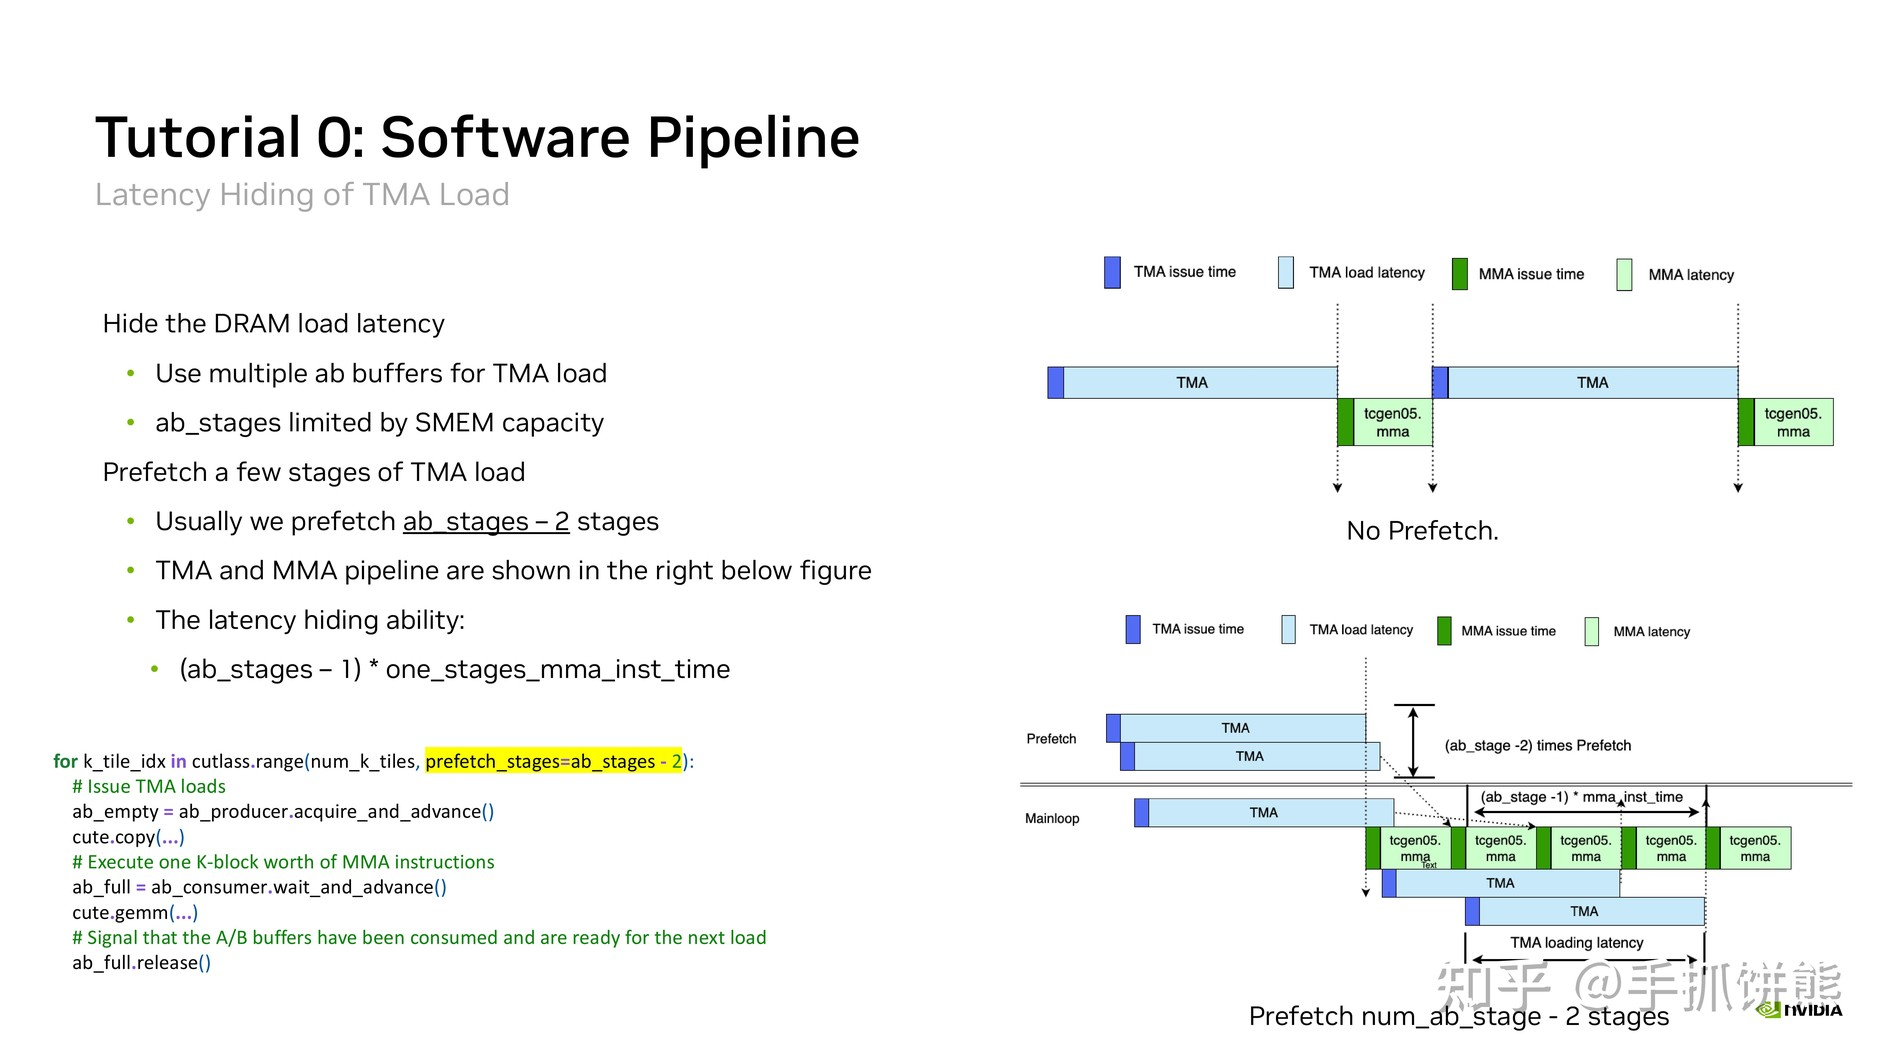
\includegraphics[width=0.9\textwidth]{figures/zhaoshangchun-03-cutlass-python/fig-12.jpg}
\end{figure}

\textbf{Software Pipeline 的核心原理：}

DRAM 的加载延迟通常在 \textbf{数百到上千个时钟周期}，如果不做隐藏，Tensor Core 将在等待数据时处于空闲状态。Software Pipeline 通过以下机制隐藏延迟：

\textbf{多缓冲机制（Multi-buffering）：}

\begin{itemize}
\item 使用多个 SMEM 缓冲区（ab\_\allowbreak{}stages 个）来交替存放 TMA 加载的数据
\item 受 SMEM 容量限制，缓冲区数量有限
\end{itemize}

\textbf{预取策略（Prefetching）：}

\begin{itemize}
\item 通常预取 \texttt{ab\_\allowbreak{}stages - 2} 个 stage 的数据
\item 延迟隐藏能力 = \texttt{(\allowbreak{}a\allowbreak{}b\allowbreak{}\_\allowbreak{}s\allowbreak{}t\allowbreak{}a\allowbreak{}g\allowbreak{}e\allowbreak{}s\allowbreak{} \allowbreak{}-\allowbreak{} \allowbreak{}1\allowbreak{})\allowbreak{} \allowbreak{}×\allowbreak{} \allowbreak{}o\allowbreak{}n\allowbreak{}e\allowbreak{}\_\allowbreak{}s\allowbreak{}t\allowbreak{}a\allowbreak{}g\allowbreak{}e\allowbreak{}\_\allowbreak{}m\allowbreak{}m\allowbreak{}a\allowbreak{}\_\allowbreak{}i\allowbreak{}n\allowbreak{}s\allowbreak{}t\allowbreak{}\_\allowbreak{}t\allowbreak{}i\allowbreak{}m\allowbreak{}e}
\end{itemize}

\textbf{代码实现的关键结构：}

\begin{lstlisting}
for k_tile_idx in cutlass.range(num_k_tiles, prefetch_stages=ab_stages - 2):
    # Issue TMA loads
    ab_empty = ab_producer.acquire_and_advance()
    cute.copy(...)
    # Execute one K-block worth of MMA instructions
    ab_full = ab_consumer.wait_and_advance()
    cute.gemm(...)
    # Signal buffer consumed
    ab_full.release()
\end{lstlisting}

这里使用了 \textbf{Producer-Consumer} 模型：

\begin{itemize}
\item Producer 负责 TMA 加载，获取空缓冲区后发起异步拷贝
\item Consumer 负责 MMA 计算，等待缓冲区数据就绪后执行计算
\item 计算完成后释放缓冲区供 Producer 复用
\end{itemize}

\subsection{3.3 Tutorial 0 的不足：延迟隐藏能力有限}

\begin{figure}[H]\centering
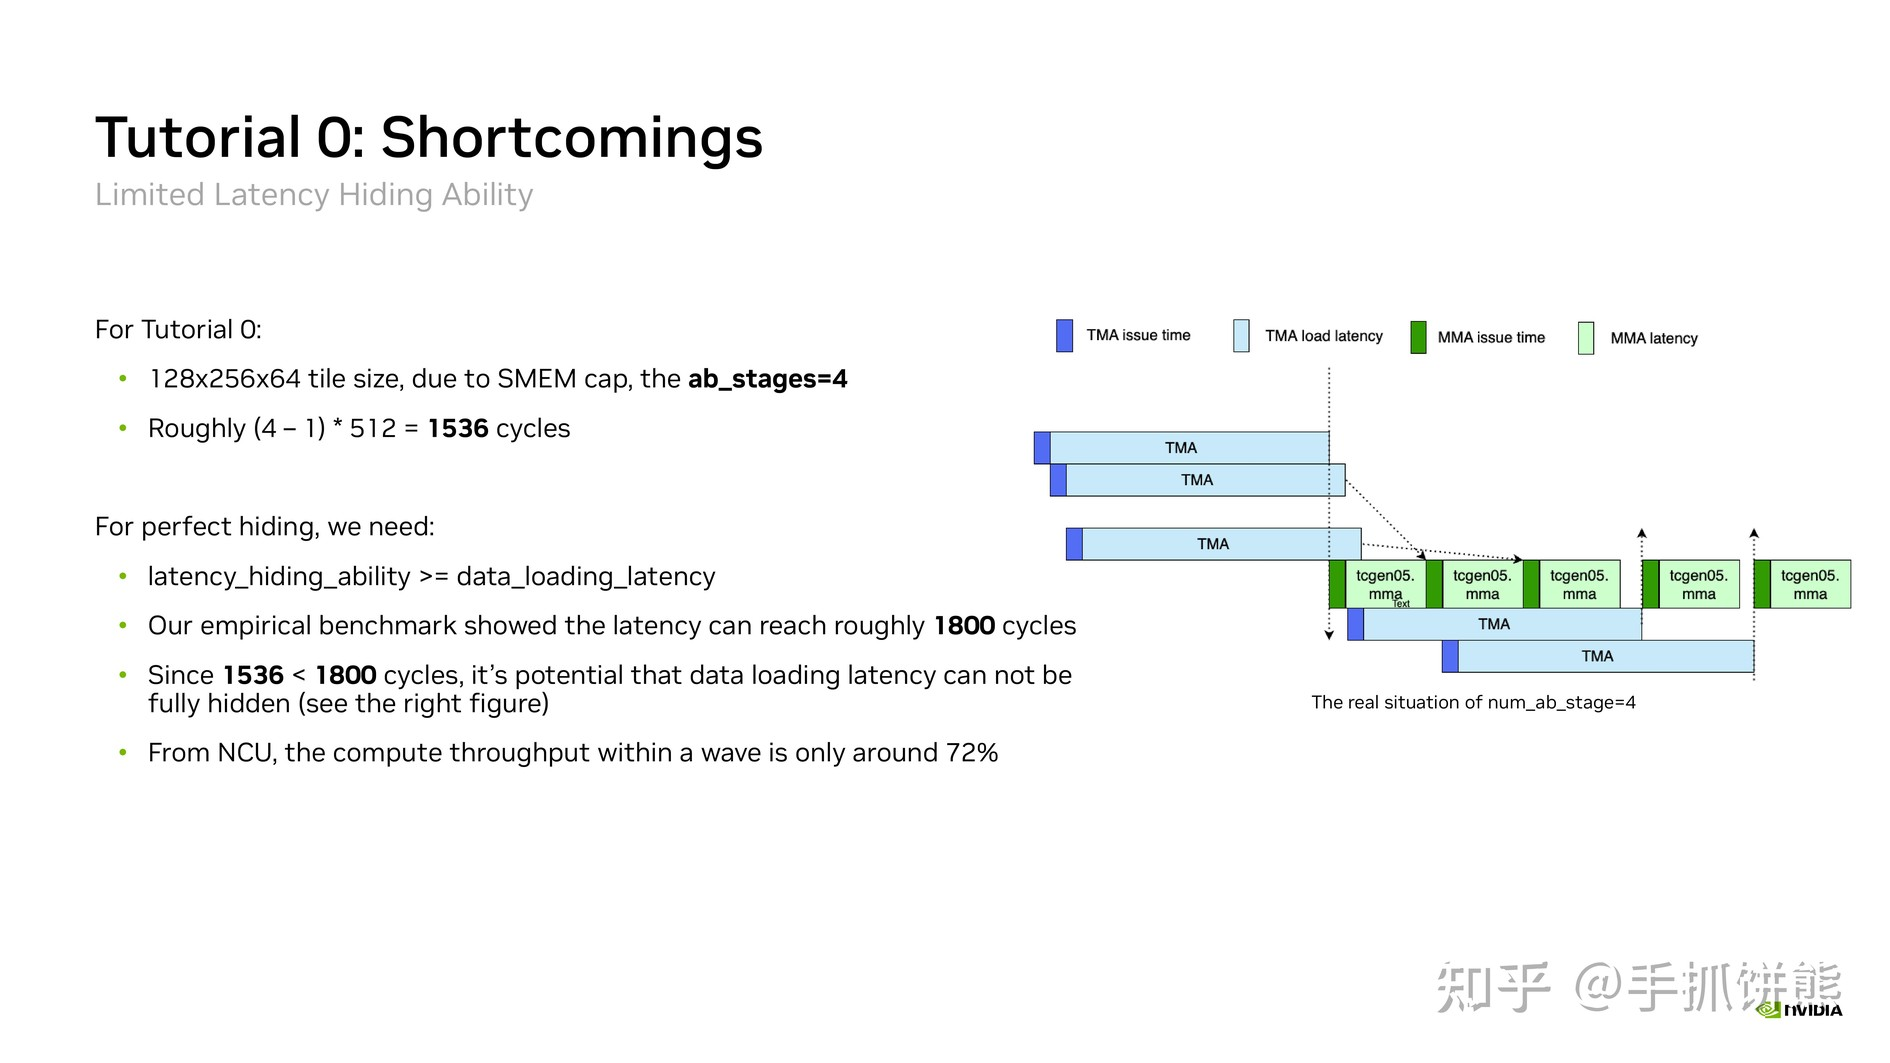
\includegraphics[width=0.9\textwidth]{figures/zhaoshangchun-03-cutlass-python/fig-13.jpg}
\end{figure}

\textbf{Tutorial 0 的瓶颈分析：}

对于 Tutorial 0 的配置（128×256×64 tile size）：

\begin{itemize}
\item 受 SMEM 容量限制，ab\_\allowbreak{}stages 最多为 4
\item 延迟隐藏能力：\texttt{(\allowbreak{}4\allowbreak{} \allowbreak{}-\allowbreak{} \allowbreak{}1\allowbreak{})\allowbreak{} \allowbreak{}×\allowbreak{} \allowbreak{}5\allowbreak{}1\allowbreak{}2\allowbreak{} \allowbreak{}=\allowbreak{} \allowbreak{}1\allowbreak{}5\allowbreak{}3\allowbreak{}6\allowbreak{} \allowbreak{}c\allowbreak{}y\allowbreak{}c\allowbreak{}l\allowbreak{}e\allowbreak{}s}
\end{itemize}

\textbf{完美隐藏条件：} latency\_\allowbreak{}hiding\_\allowbreak{}ability >=geq data\_\allowbreak{}loading\_\allowbreak{}latenc

然而实际测量表明：

\begin{itemize}
\item 数据加载延迟约为 \textbf{1800 cycles}
\item 由于 1536 < 1800 cycles，\textbf{数据加载延迟无法被完全隐藏}
\end{itemize}

\textbf{NCU（Nsight Compute）分析结果：}

\begin{itemize}
\item 波内计算吞吐量仅约 \textbf{72\%}
\item 图中右侧的时间线清楚展示了当 ab\_\allowbreak{}stages=4 时，MMA 执行存在明显的停顿（stall），等待数据加载完成
\end{itemize}

这个分析直接引出了 Tutorial 1 的优化方向：如何增加延迟隐藏能力。

\subsection{3.4 Tutorial 1：启用 2CTA（tcgen05.2cta）}

\begin{figure}[H]\centering
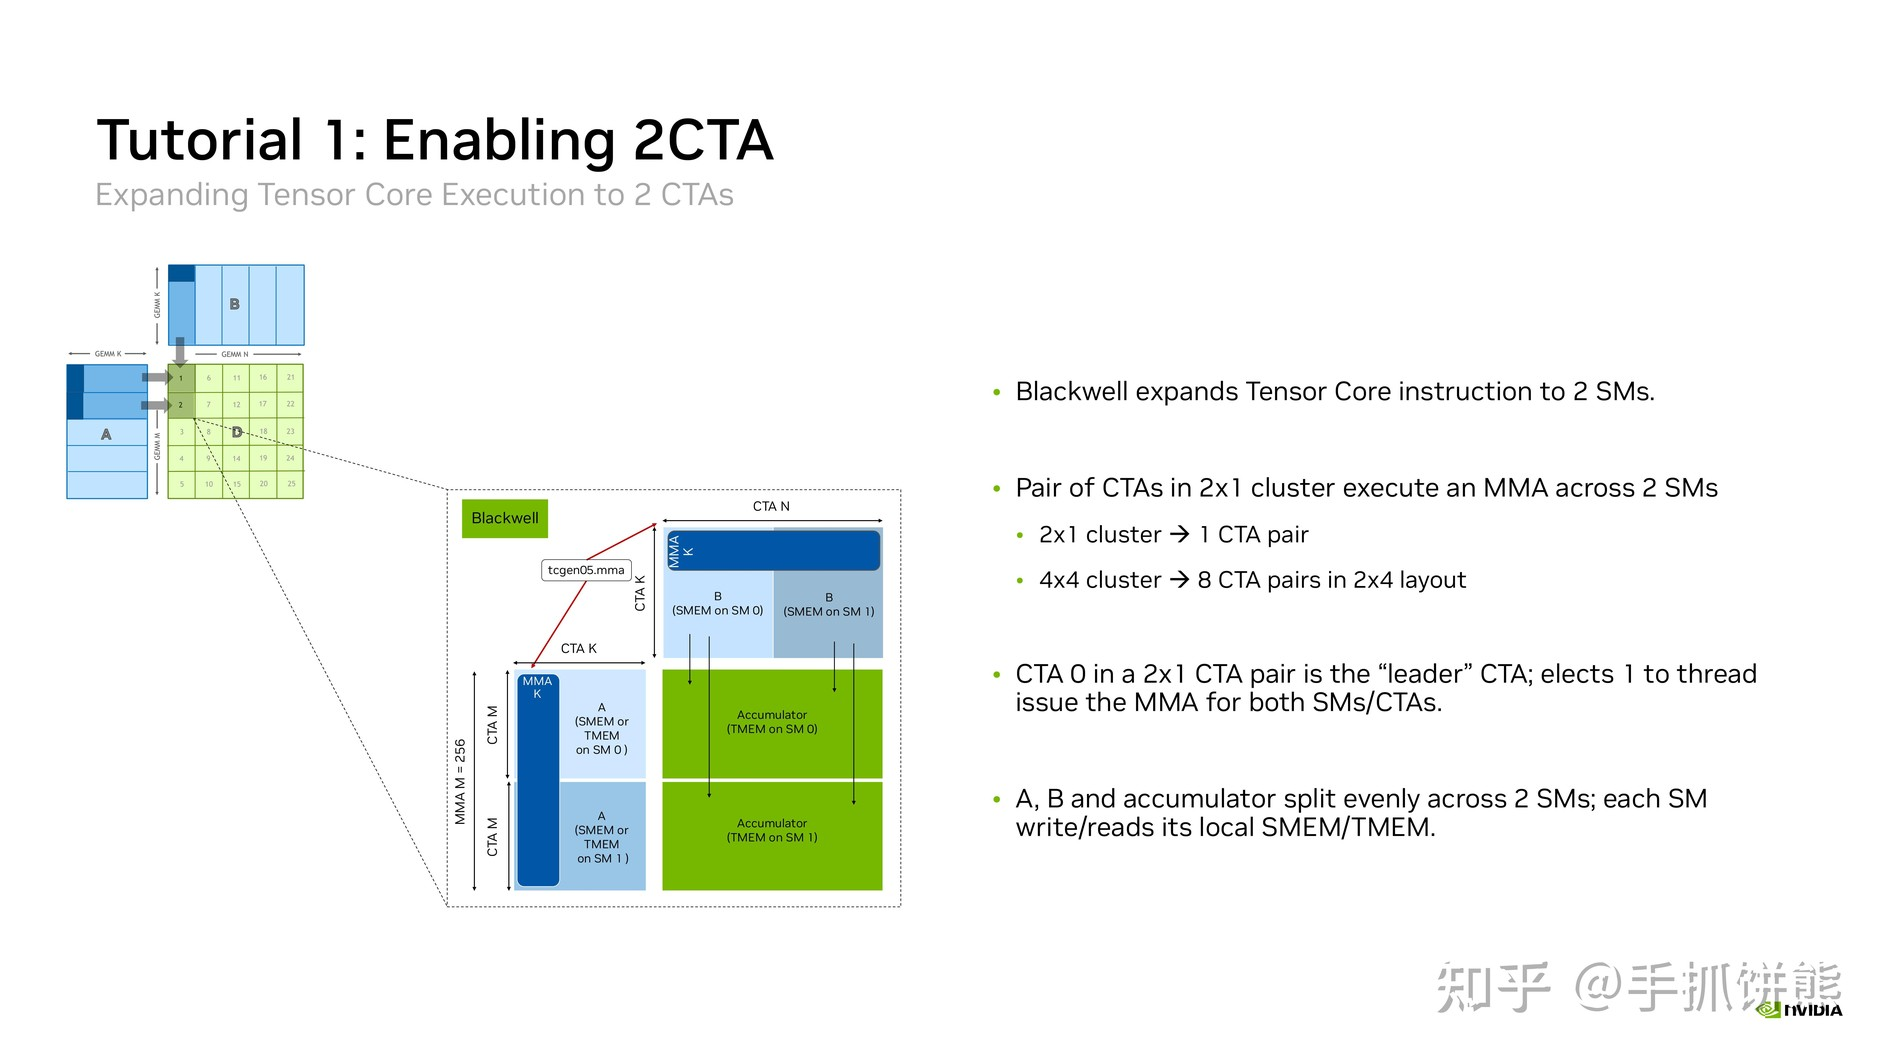
\includegraphics[width=0.9\textwidth]{figures/zhaoshangchun-03-cutlass-python/fig-14.jpg}
\end{figure}

\textbf{Blackwell 2\allowbreak{}CTA 技术原理：}

Blackwell 架构引入了一项重要的硬件创新——\textbf{将 Tensor Core 执行扩展到 2 个 CTA（Cooperative Thread Array）}：

\textbf{核心概念：}

\begin{itemize}
\item 一对 CTA 在同一 TPC（Texture Processing Cluster）的 2 个 SM 上协同执行一次 MMA
\item 2×1 cluster 包含 1 个 CTA pair
\item 4×4 cluster 包含 8 个 CTA pairs（2×4 布局）
\end{itemize}

\textbf{执行机制：}

\begin{itemize}
\item 2×1 CTA pair 中的 CTA 0 是 "leader CTA"
\item Leader CTA 选出一个线程为两个 SM/\allowbreak{}CTA 发射 MMA 指令（\texttt{tcgen05.\allowbreak{}mma}）
\item A、B 矩阵和累加器在 2 个 SM 之间均匀分割
\item 每个 SM 读写其本地的 SMEM/\allowbreak{}TMEM
\end{itemize}

\textbf{内存布局（如图所示）：}

\begin{itemize}
\item SM 0 和 SM 1 各持有 A 矩阵的一半（SMEM 或 TMEM）
\item B 矩阵在两个 SM 之间共享（关键优化点！）
\item 累加器分别存储在两个 SM 的 TMEM 中
\item MMA 维度：M=256（跨 2 个 SM），K 和 N 维度在两个 SM 内处理
\end{itemize}

\subsection{3.5 Tutorial 1：2CTA 带来的 SMEM 优化}

\begin{figure}[H]\centering
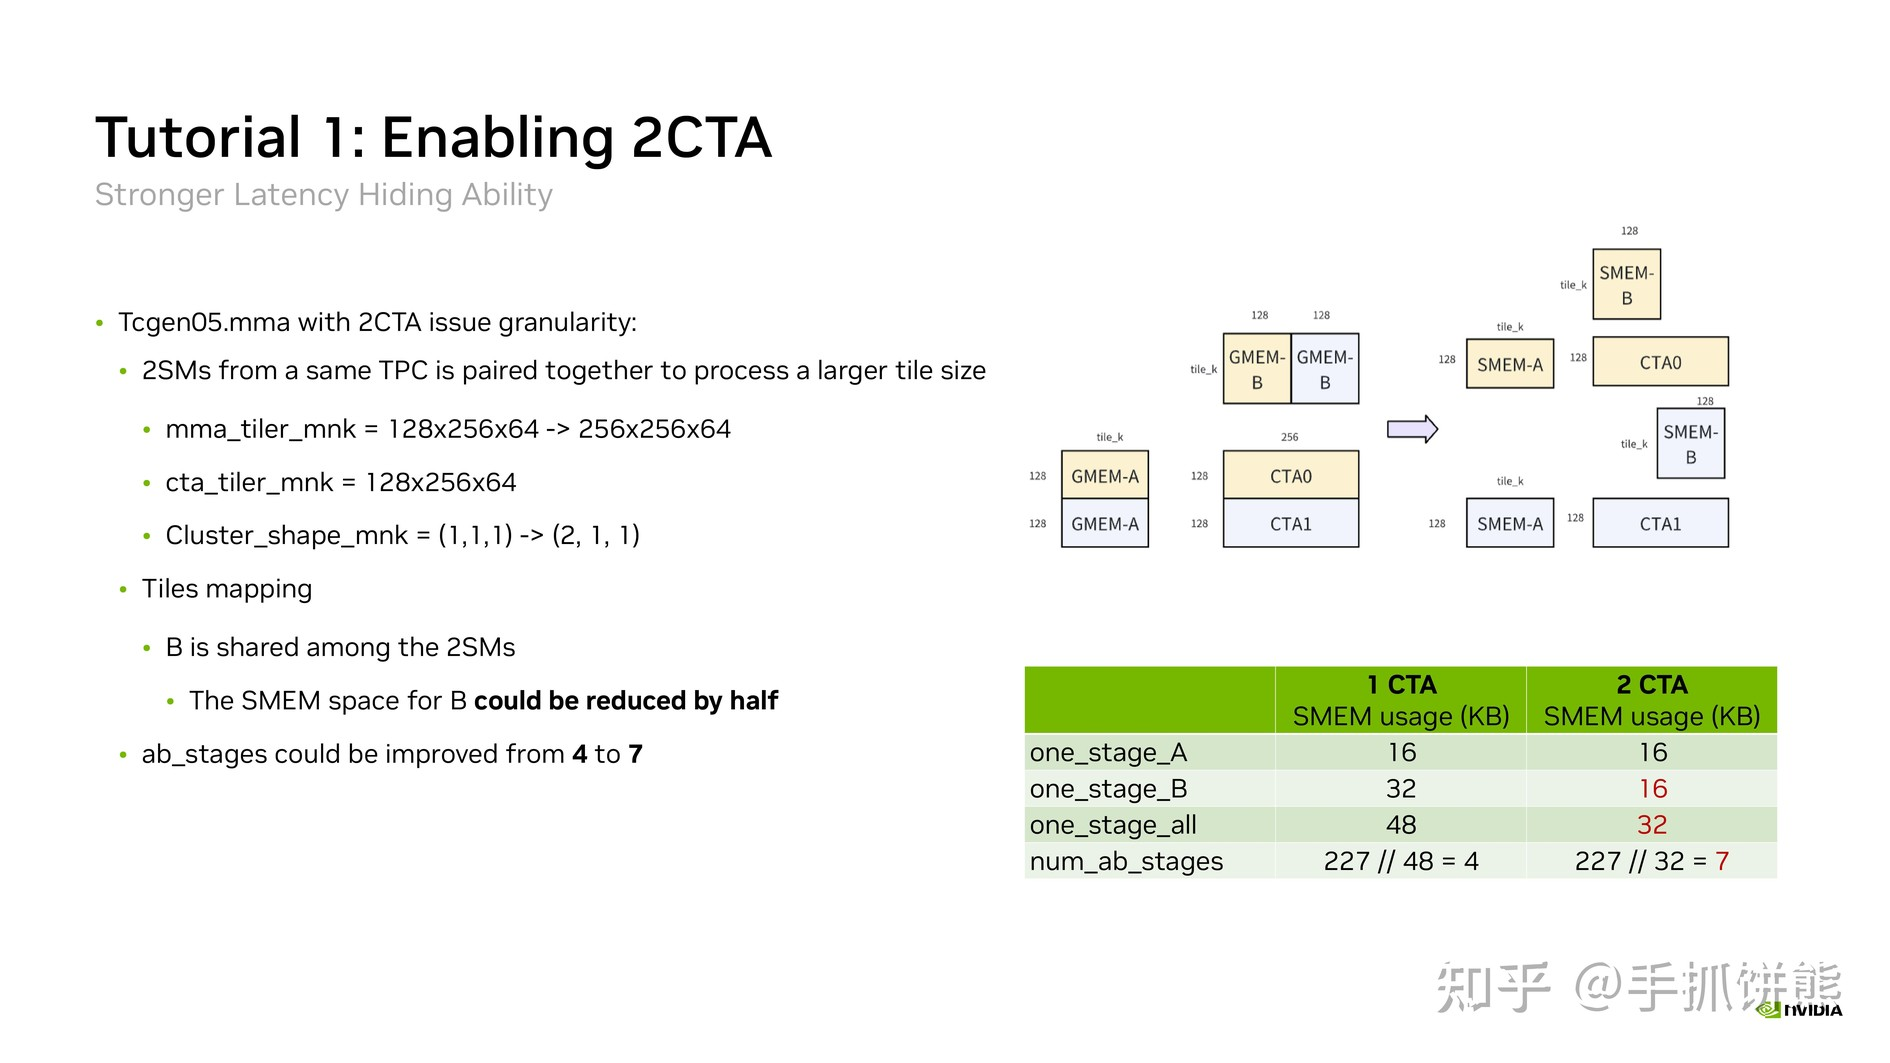
\includegraphics[width=0.9\textwidth]{figures/zhaoshangchun-03-cutlass-python/fig-15.jpg}
\end{figure}

\textbf{2\allowbreak{}CTA 的配置变化：}

启用 2\allowbreak{}CTA 后，关键参数发生如下变化：

\begin{itemize}
\item \texttt{mma\_\allowbreak{}tiler\_\allowbreak{}mnk}：128×256×64 → 256×256×64
\item \texttt{cta\_\allowbreak{}tiler\_\allowbreak{}mnk}：128×256×64（每个 CTA 的实际 tile 不变）
\item \texttt{cluster\_\allowbreak{}shape\_\allowbreak{}mnk}：(1,1,1) → (2,1,1)
\end{itemize}

\textbf{SMEM 节省的关键原因：}

由于 \textbf{B 矩阵在 2 个 SM 之间共享}，每个 SM 只需要存储一半的 B 数据：

\begin{table}[htbp]\centering\small
\begin{adjustbox}{max width=\textwidth}
\begin{tabular}{lll}
\toprule
配置项 & 1 CTA SMEM (KB) & 2 CTA SMEM (KB) \\
\midrule
one\_\allowbreak{}stage\_\allowbreak{}A & 16 & 16 \\
one\_\allowbreak{}stage\_\allowbreak{}B & 32 & 16 \\
one\_\allowbreak{}stage\_\allowbreak{}all & 48 & 32 \\
num\_\allowbreak{}ab\_\allowbreak{}stages & 227 /\allowbreak{}/\allowbreak{} 48 = 4 & 227 /\allowbreak{}/\allowbreak{} 32 = 7 \\
\bottomrule
\end{tabular}
\end{adjustbox}
\end{table}

\textbf{延迟隐藏能力提升：}

\begin{itemize}
\item 原来：(4-1) × 512 = 1536 cycles
\item 现在：(7-1) × 512 = \textbf{3072 cycles}
\end{itemize}

ab\_\allowbreak{}stages 从 4 提升到 7，延迟隐藏能力翻倍，远超 1800 cycles 的加载延迟，理论上可以完全隐藏 DRAM 延迟。

\subsection{3.6 Tutorial 1：性能结果}

\begin{figure}[H]\centering
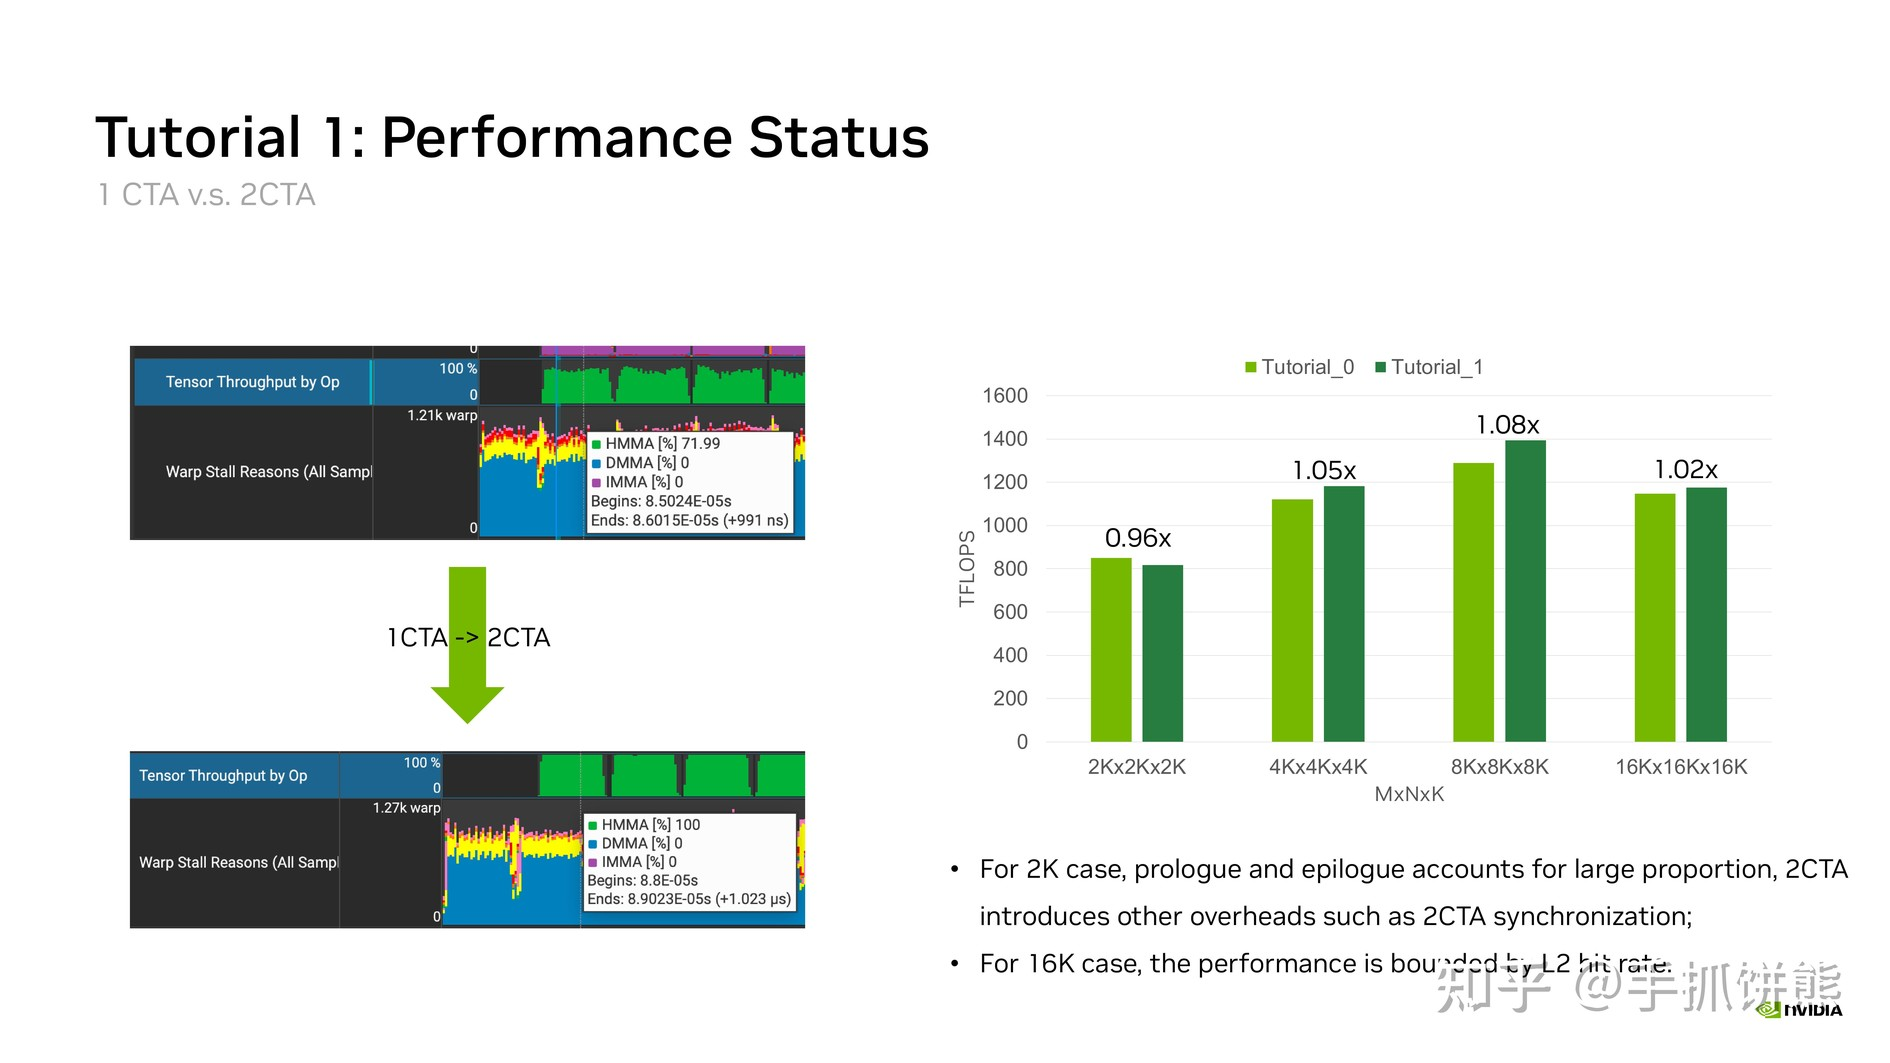
\includegraphics[width=0.9\textwidth]{figures/zhaoshangchun-03-cutlass-python/fig-16.jpg}
\end{figure}

\textbf{1\allowbreak{}CTA vs 2\allowbreak{}CTA 性能对比：}

\begin{itemize}
\item \textbf{2\allowbreak{}K×2\allowbreak{}K×2\allowbreak{}K：} 0.96x（略有下降）——因为 prologue 和 epilogue 占比较大，2\allowbreak{}CTA 引入的同步开销反而成为负担
\item \textbf{4\allowbreak{}K×4\allowbreak{}K×4\allowbreak{}K：} 1.05x 提升
\item \textbf{8\allowbreak{}K×8\allowbreak{}K×8\allowbreak{}K：} 1.08x 提升——主循环占比增大，延迟隐藏优势显现
\item \textbf{16\allowbreak{}K×16\allowbreak{}K×16\allowbreak{}K：} 1.02x（提升有限）——性能受限于 \textbf{L2 缓存命中率}
\end{itemize}

\textbf{关键洞察：} 2\allowbreak{}CTA 优化的收益在中等规模（4\allowbreak{}K-8\allowbreak{}K）最为明显。对于小规模，同步开销主导；对于大规模，L2 缓存成为新的瓶颈。这体现了 GEMM 优化中"瓶颈灵活性"的特点——不同规模有不同的性能瓶颈。

\subsection{3.7 Tutorial 2：Epilogue 优化——TMA Store}

\begin{figure}[H]\centering
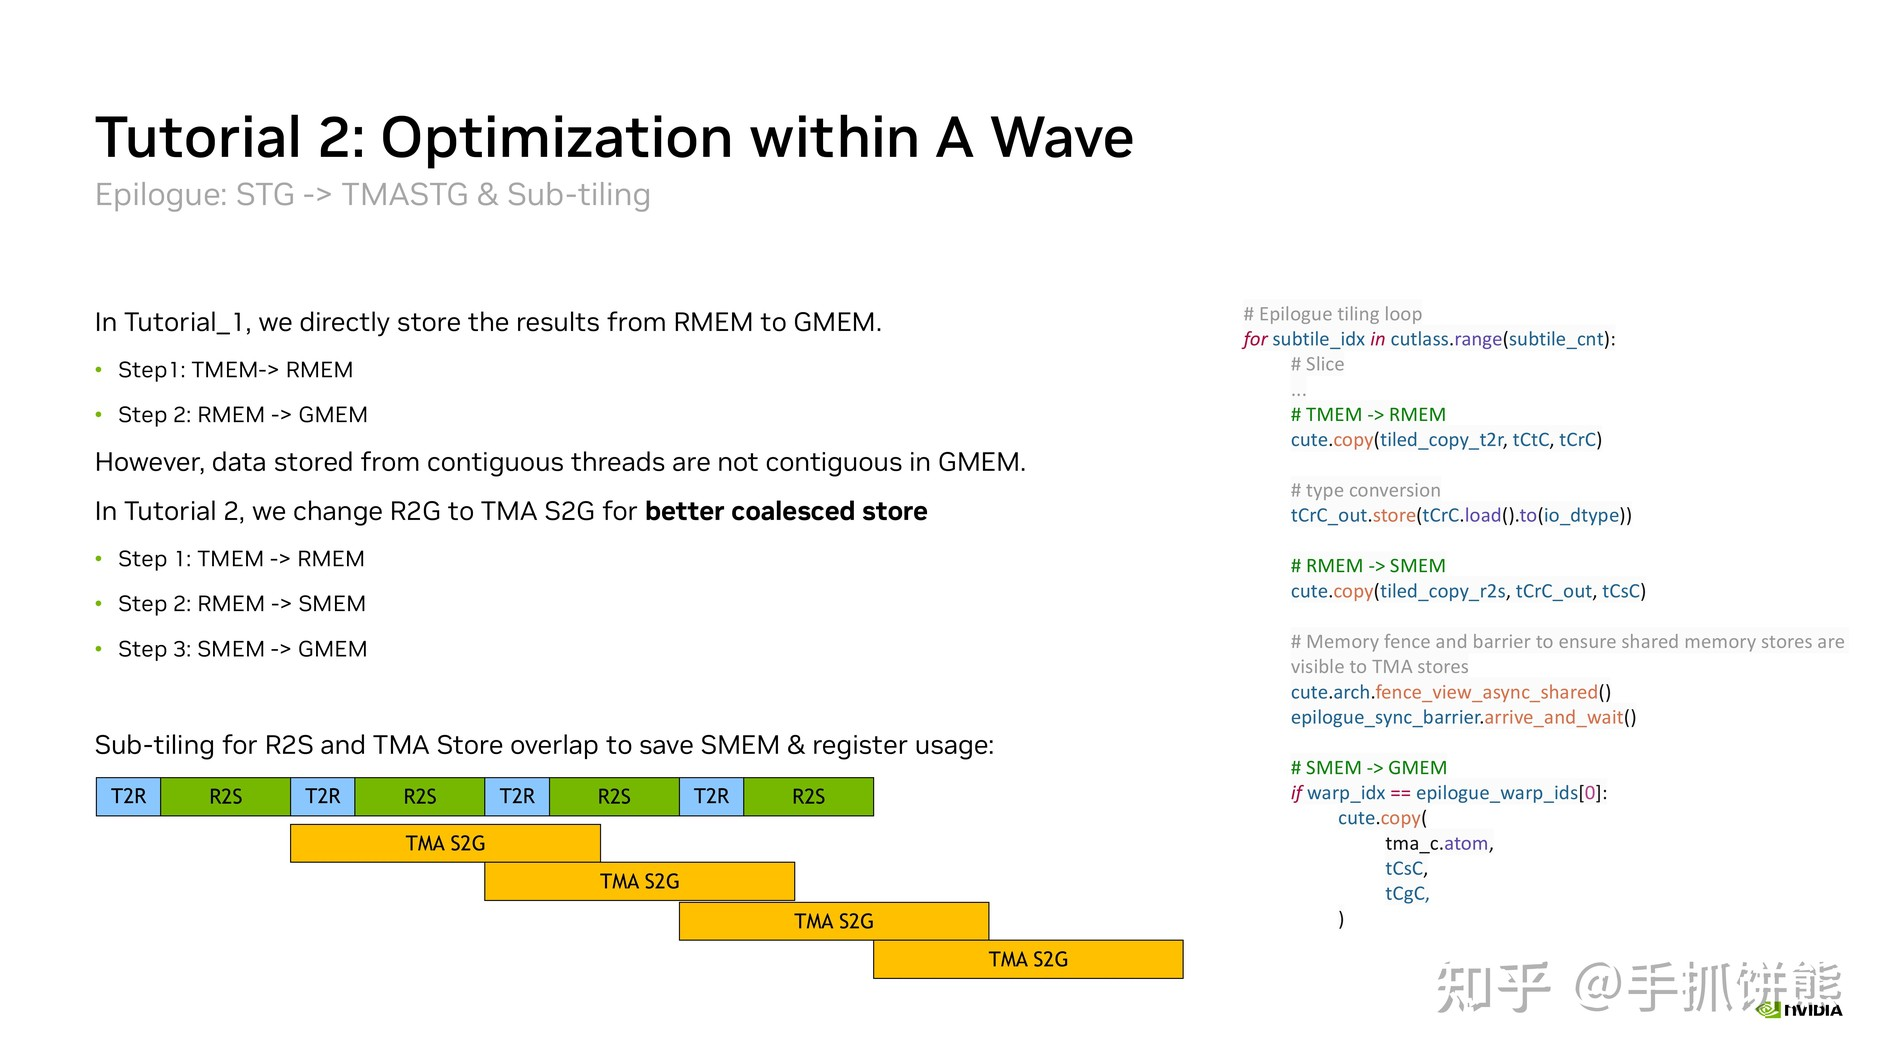
\includegraphics[width=0.9\textwidth]{figures/zhaoshangchun-03-cutlass-python/fig-17.jpg}
\end{figure}

\textbf{问题背景：}

在 Tutorial 1 中，结果从 RMEM 直接存储到 GMEM（STG 指令）。但由于连续线程的数据在 GMEM 中并不连续，这导致了非合并（non-coalesced）的内存访问，严重浪费带宽。

\textbf{优化方案：STG → TMA S2\allowbreak{}G + Sub-tiling}

Tutorial 2 将 epilogue 改为通过 TMA 进行合并存储：

\begin{itemize}
\item Step 1：TMEM → RMEM（T2\allowbreak{}R）
\item Step 2：RMEM → SMEM（R2\allowbreak{}S）
\item Step 3：SMEM → GMEM（TMA S2\allowbreak{}G，合并访问）
\end{itemize}

\textbf{Sub-tiling 策略：}

为了节省 SMEM 和寄存器使用量，采用子分块（sub-tiling）方式：将 epilogue 的输出分成多个子块，每次只处理一个子块的 T2\allowbreak{}R → R2\allowbreak{}S → TMA S2\allowbreak{}G 流水线。如图中所示，4 个子块依次执行，R2\allowbreak{}S 和 TMA S2\allowbreak{}G 可以重叠。

\textbf{核心代码结构：}

\begin{lstlisting}
for subtile_idx in cutlass.range(subtile_cnt):
    # TMEM -> RMEM
    cute.copy(tiled_copy_t2r, tCtC, tCrC)
    # Type conversion
    tCrC_out.store(tCrC.load().to(io_dtype))
    # RMEM -> SMEM
    cute.copy(tiled_copy_r2s, tCrC_out, tCsC)
    # Memory fence
    cute.arch.fence_view_async_shared()
    epilogue_sync_barrier.arrive_and_wait()
    # SMEM -> GMEM (TMA)
    if warp_idx == epilogue_warp_ids[0]:
        cute.copy(tma_c.atom, tCsC, tCgC)
\end{lstlisting}

\subsection{3.8 Tutorial 2：Epilogue 时间线优化效果}

\begin{figure}[H]\centering
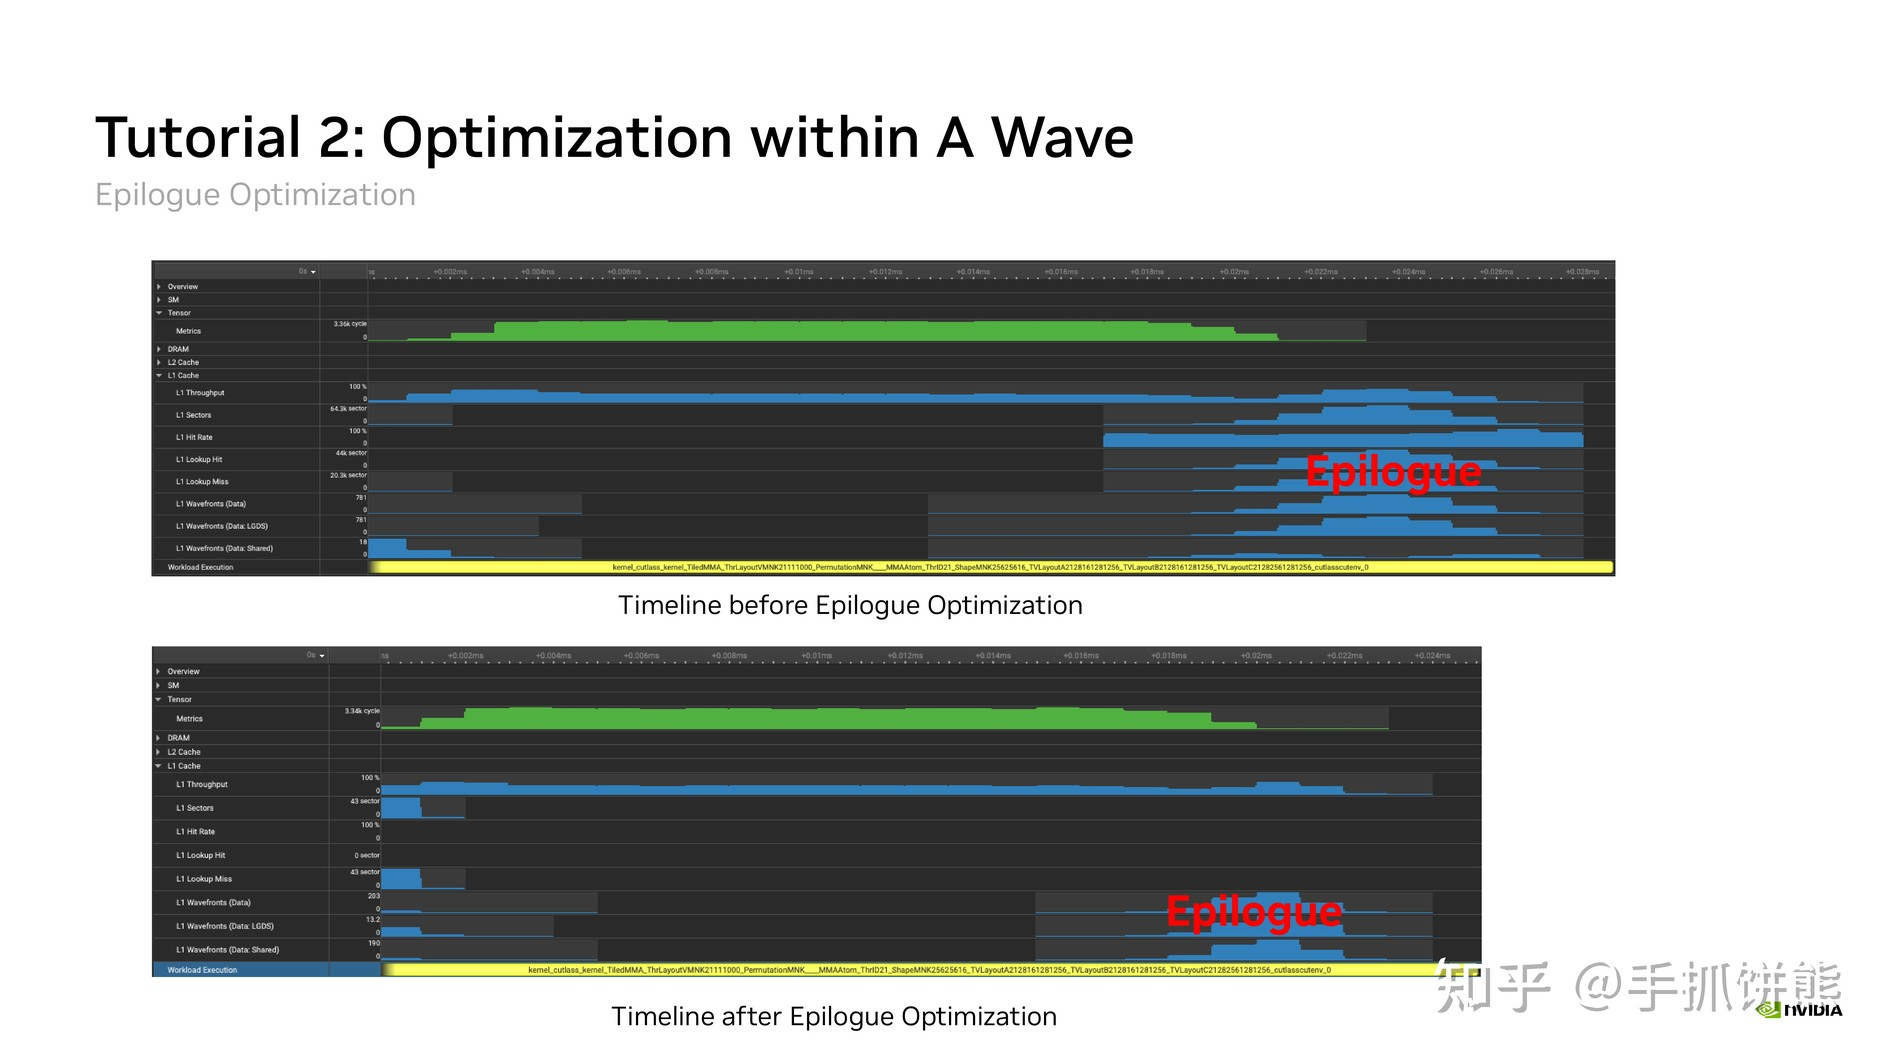
\includegraphics[width=0.9\textwidth]{figures/zhaoshangchun-03-cutlass-python/fig-18.jpg}
\end{figure}

\textbf{时间线对比：}

该图清晰展示了 epilogue 优化前后的执行时间线：

\begin{itemize}
\item \textbf{优化前：} Epilogue 阶段占据较长时间，因为非合并内存访问导致大量带宽浪费
\item \textbf{优化后：} Epilogue 时间显著缩短，TMA 合并存储的效率远高于逐线程存储
\end{itemize}

这一优化对小 K 值（epilogue 占比较大）的场景尤为重要。

\subsection{3.9 Tutorial 2：Warp Specialization}

\begin{figure}[H]\centering
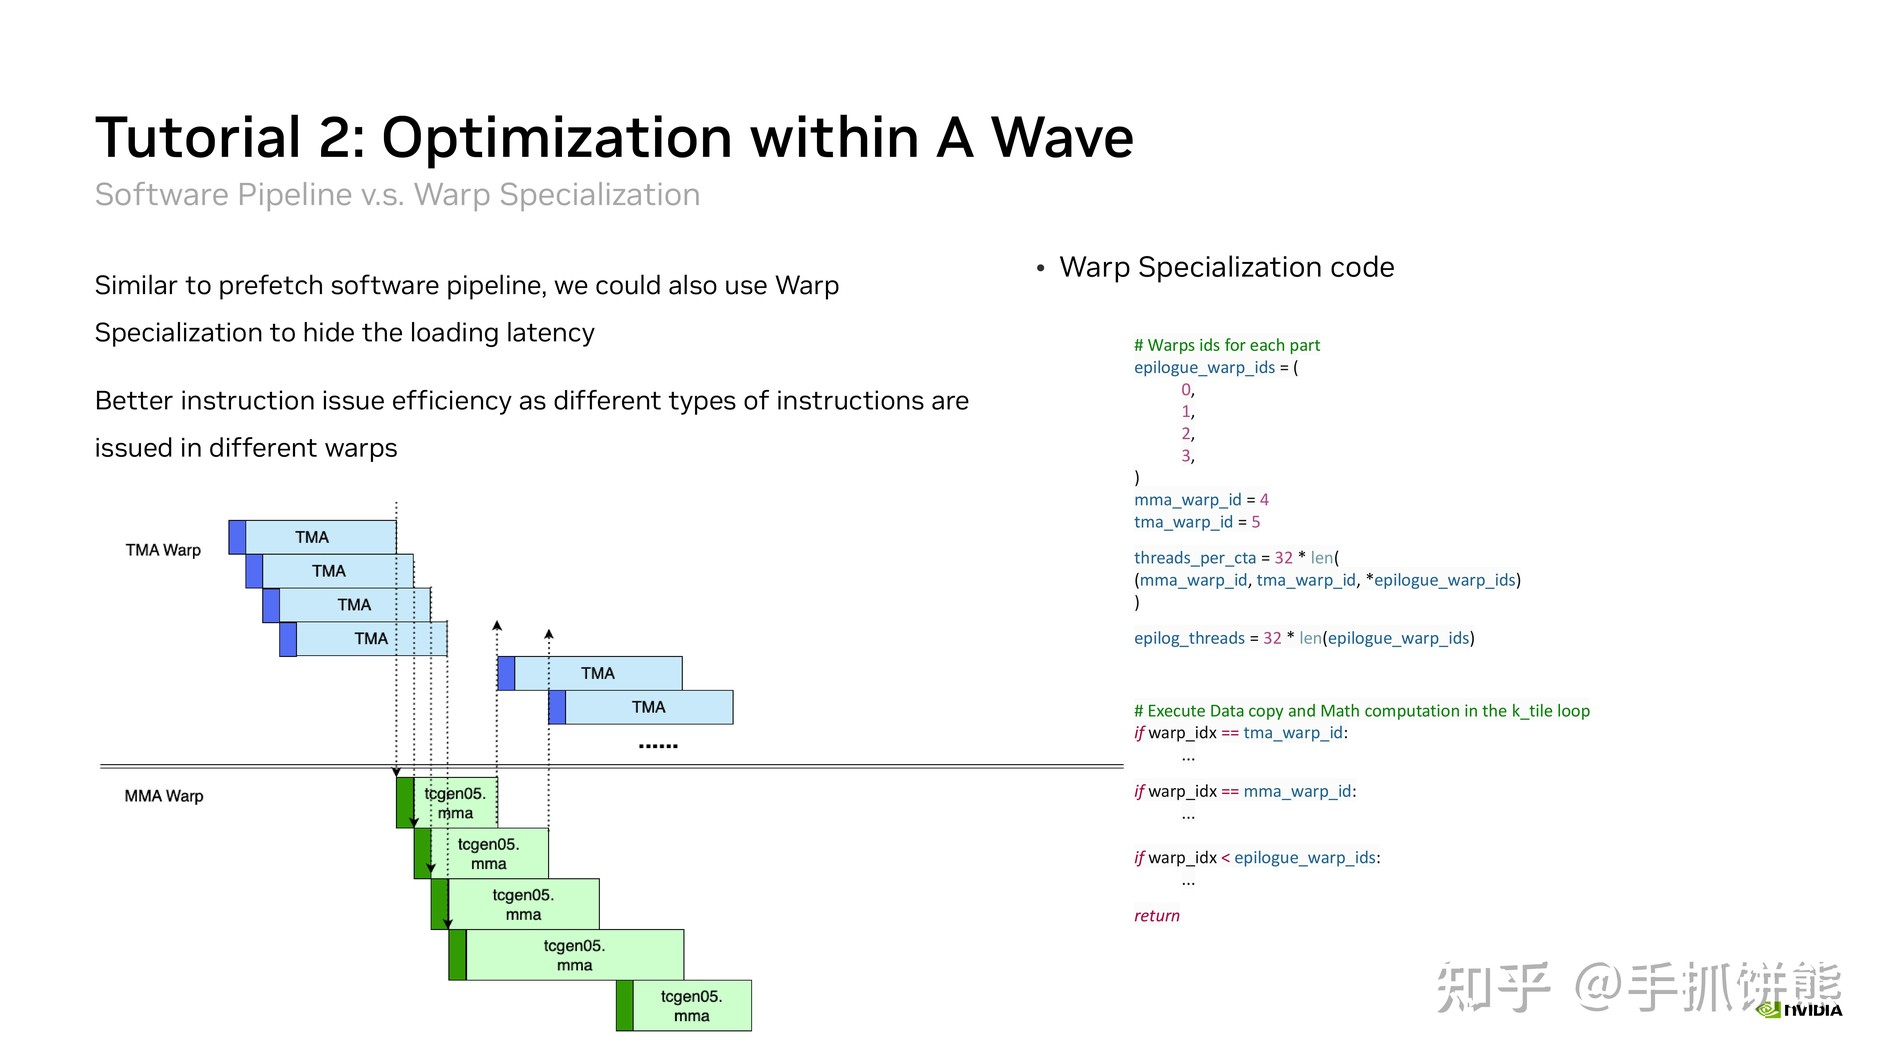
\includegraphics[width=0.9\textwidth]{figures/zhaoshangchun-03-cutlass-python/fig-19.jpg}
\end{figure}

\textbf{Software Pipeline vs Warp Specialization：}

除了 Software Pipeline 预取机制外，\textbf{Warp Specialization} 提供了另一种隐藏延迟的方式：

\textbf{核心思想：} 将不同类型的指令分配给不同的 warp 执行，实现任务级并行。

\textbf{Warp 分配方案：}

\begin{lstlisting}
epilogue_warp_ids = (0, 1, 2, 3)  # 4 个 warp 处理 epilogue
mma_warp_id = 4                    # 1 个 warp 处理 MMA
tma_warp_id = 5                    # 1 个 warp 处理 TMA
threads_per_cta = 32 * 6           # 共 6 个 warp = 192 线程
\end{lstlisting}

\textbf{优势：}

\begin{itemize}
\item \textbf{更好的指令发射效率：} 不同类型的指令（TMA load、MMA compute、TMA store）由专用 warp 发射，避免指令队列拥塞
\item \textbf{隐藏 epilogue 开销：} 当 MMA warp 还在计算时，epilogue warp 可以处理上一次迭代的结果写回
\end{itemize}

\textbf{执行模式：}

\begin{lstlisting}
if warp_idx == tma_warp_id:
    ...  # 负责所有 TMA 加载操作
if warp_idx == mma_warp_id:
    ...  # 负责所有 MMA 计算操作
if warp_idx < epilogue_warp_ids:
    ...  # 负责结果写回操作
\end{lstlisting}

\subsection{3.10 Tutorial 2：性能提升}

\begin{figure}[H]\centering
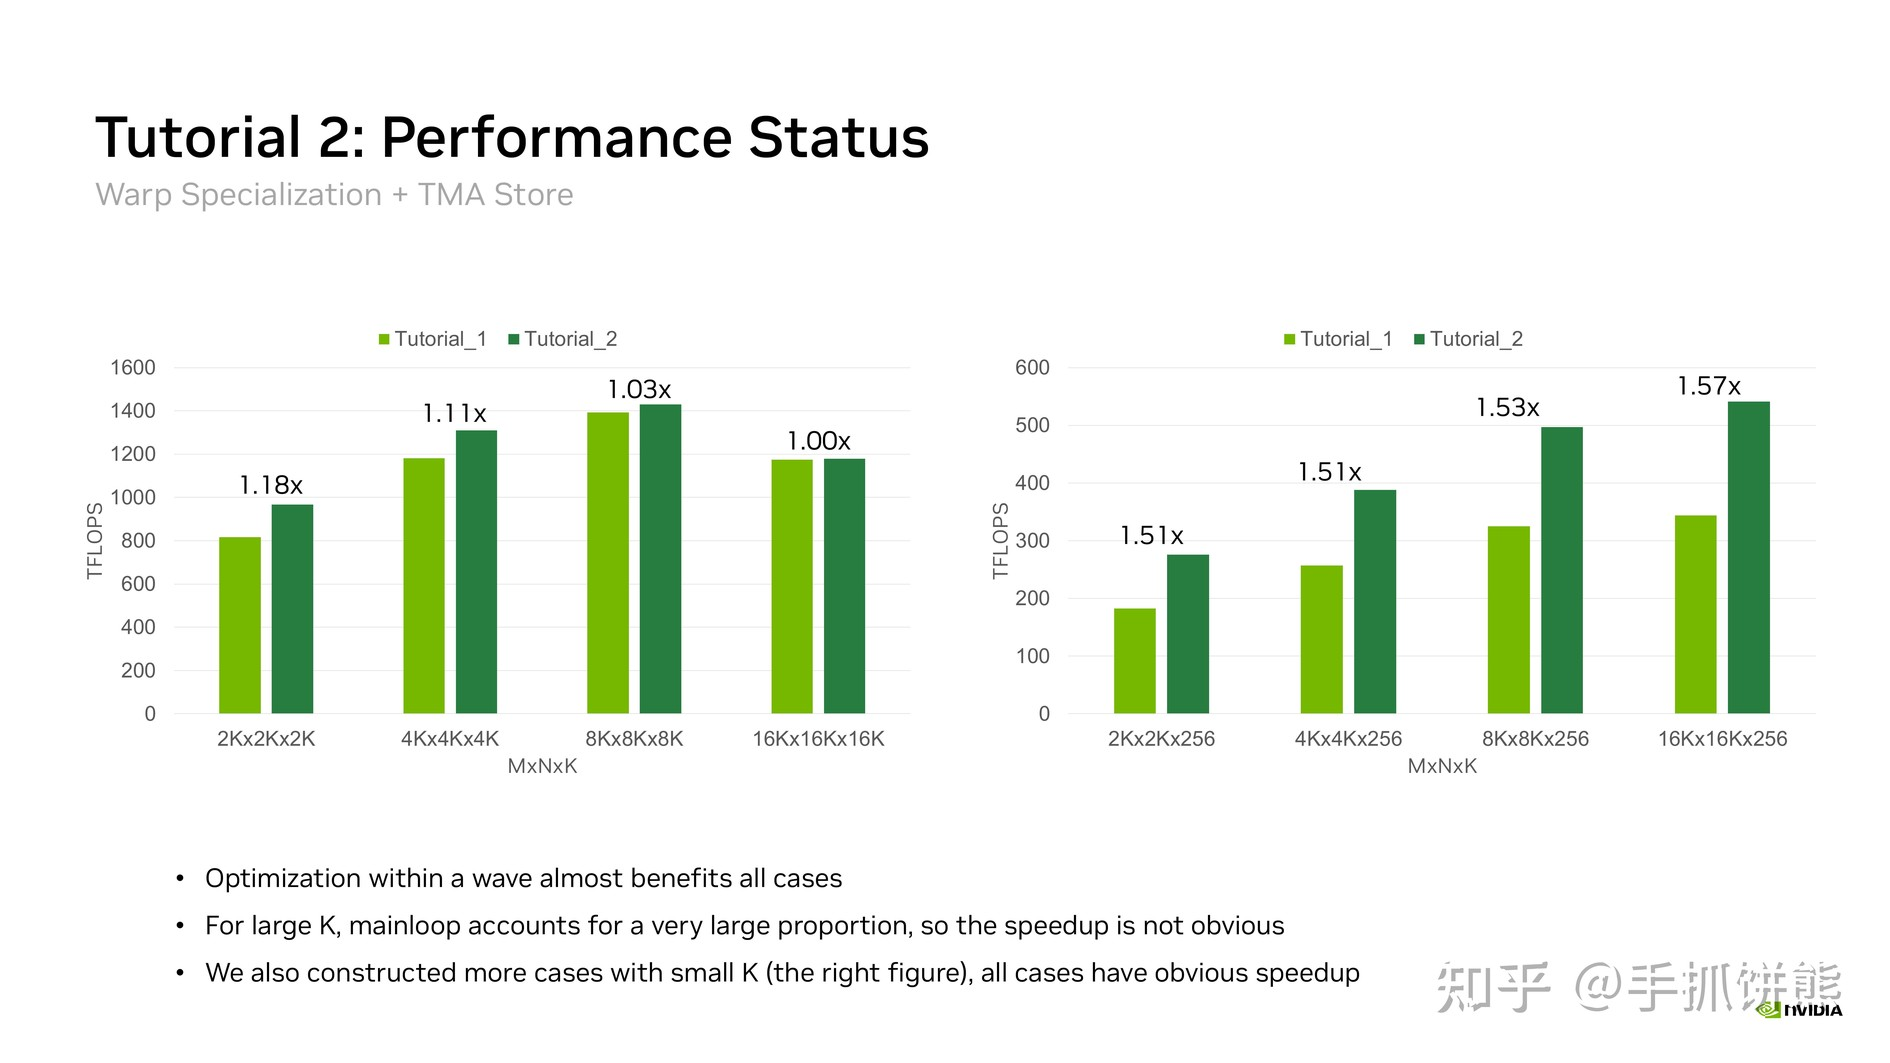
\includegraphics[width=0.9\textwidth]{figures/zhaoshangchun-03-cutlass-python/fig-20.jpg}
\end{figure}

\textbf{Warp Specialization + TMA Store 的性能收益：}

\textbf{大 K 场景（左图，Kx\allowbreak{}Kx\allowbreak{}K）：}

\begin{itemize}
\item 2\allowbreak{}K×2\allowbreak{}K×2\allowbreak{}K：1.18x 提升
\item 4\allowbreak{}K×4\allowbreak{}K×4\allowbreak{}K：1.11x 提升
\item 8\allowbreak{}K×8\allowbreak{}K×8\allowbreak{}K：1.03x 提升
\item 16\allowbreak{}K×16\allowbreak{}K×16\allowbreak{}K：1.00x（几乎无提升）
\end{itemize}

对于大 K 值，mainloop 占据绝大比例，因此 epilogue 和 prologue 的优化效果不明显。 \textbf{小 K 场景（右图，Kx\allowbreak{}Kx256）：}

\begin{itemize}
\item 2\allowbreak{}K×2\allowbreak{}K×256：1.51x 提升
\item 4\allowbreak{}K×4\allowbreak{}K×256：1.51x 提升
\item 8\allowbreak{}K×8\allowbreak{}K×256：1.53x 提升
\item 16\allowbreak{}K×16\allowbreak{}K×256：1.57x 提升
\end{itemize}

\textbf{关键发现：} 当 K 维度较小时，epilogue 占据了内核执行时间的大比例，Warp Specialization + TMA Store 的优化效果极为显著（超过 1.5x）。这在实际 LLM 推理中的 prefill 阶段（通常 K=hidden\_\allowbreak{}dim，相对较小）非常有价值。

\subsection{3.11 Tutorial 3：Persistent Kernel——波间重叠优化}

\begin{figure}[H]\centering
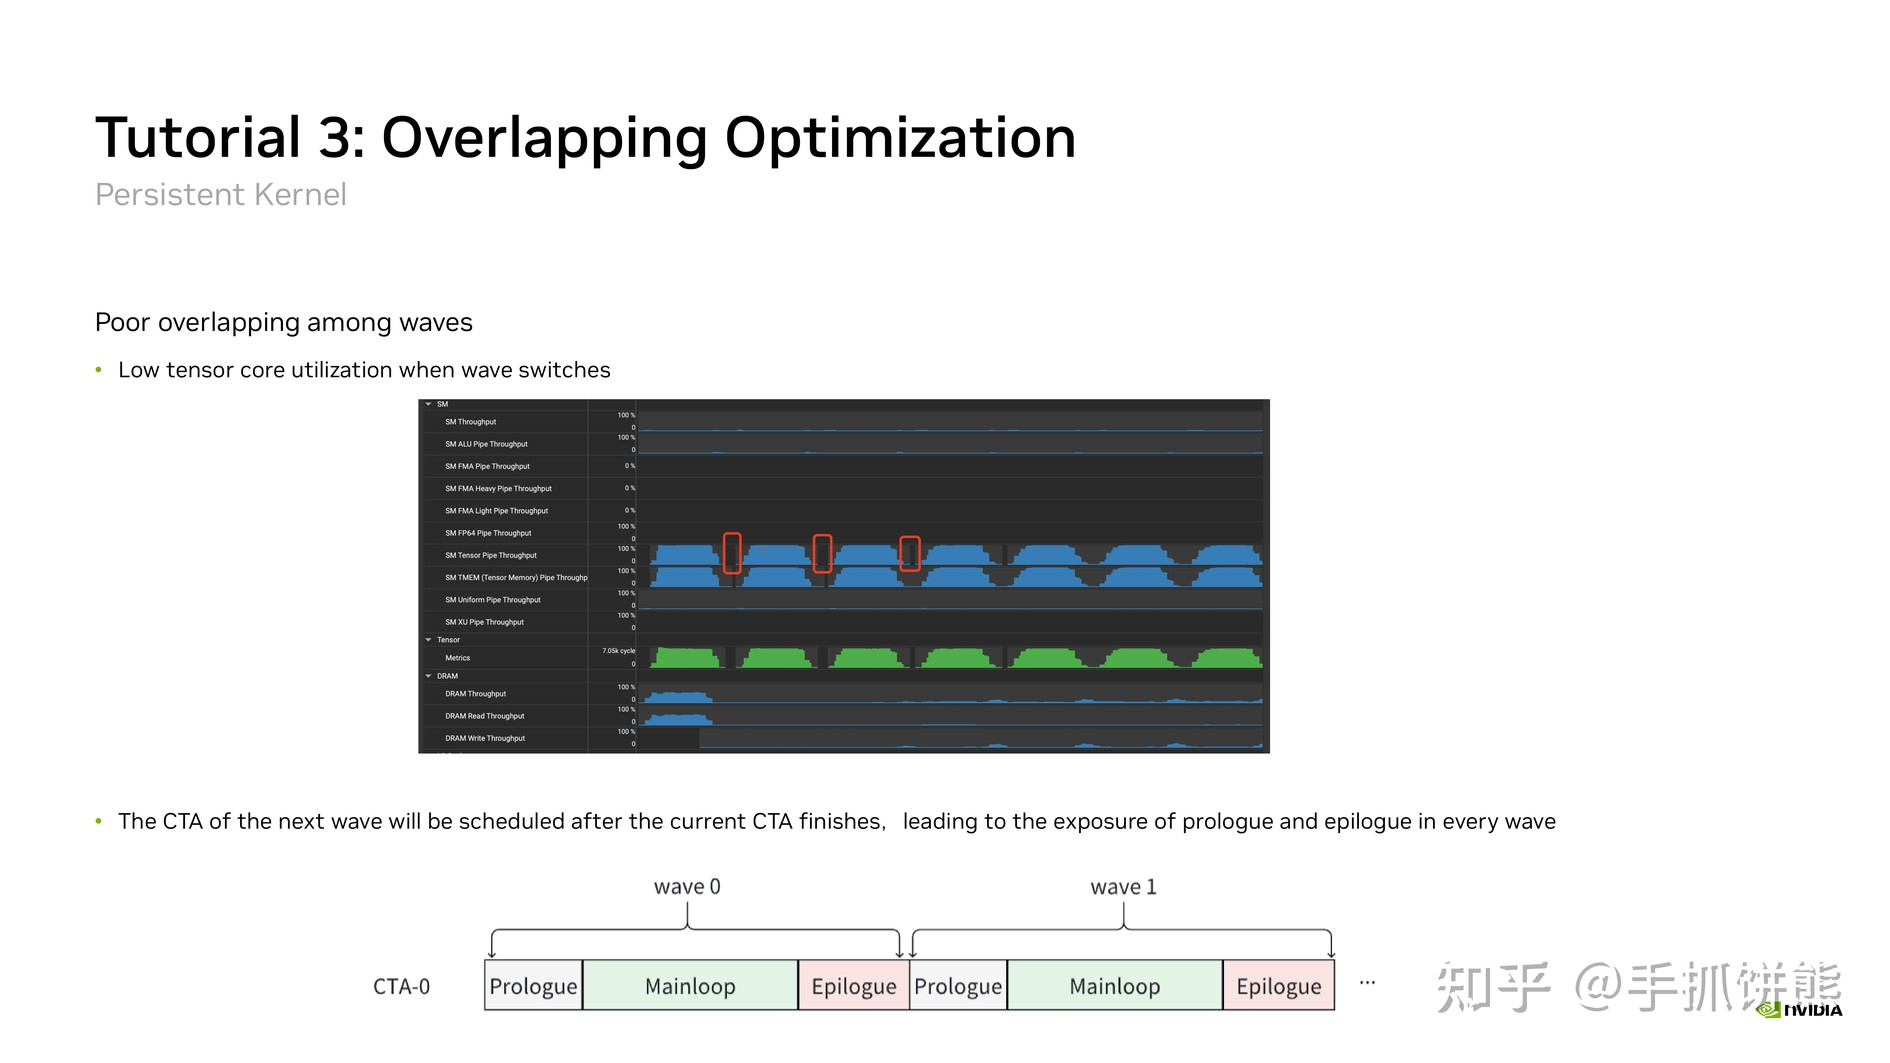
\includegraphics[width=0.9\textwidth]{figures/zhaoshangchun-03-cutlass-python/fig-21.jpg}
\end{figure}

\textbf{波间切换的问题：}

在非 Persistent 模式下，GEMM 的 tile 被分成多个 "wave" 执行：

\begin{itemize}
\item 当一个 wave 中的所有 CTA 执行完毕后，下一个 wave 的 CTA 才会被调度
\item 这导致每个 wave 的 \textbf{prologue 和 epilogue 都暴露在关键路径}上
\item wave 切换时 Tensor Core 利用率极低
\end{itemize}

图中展示了这种"阶梯式"执行模式：每个 wave 的 prologue（数据预取）和 epilogue（结果写回）都无法与其他 wave 重叠，造成严重的计算资源浪费。

\subsection{3.12 Tutorial 3：Static Persistent Scheduler}

\begin{figure}[H]\centering
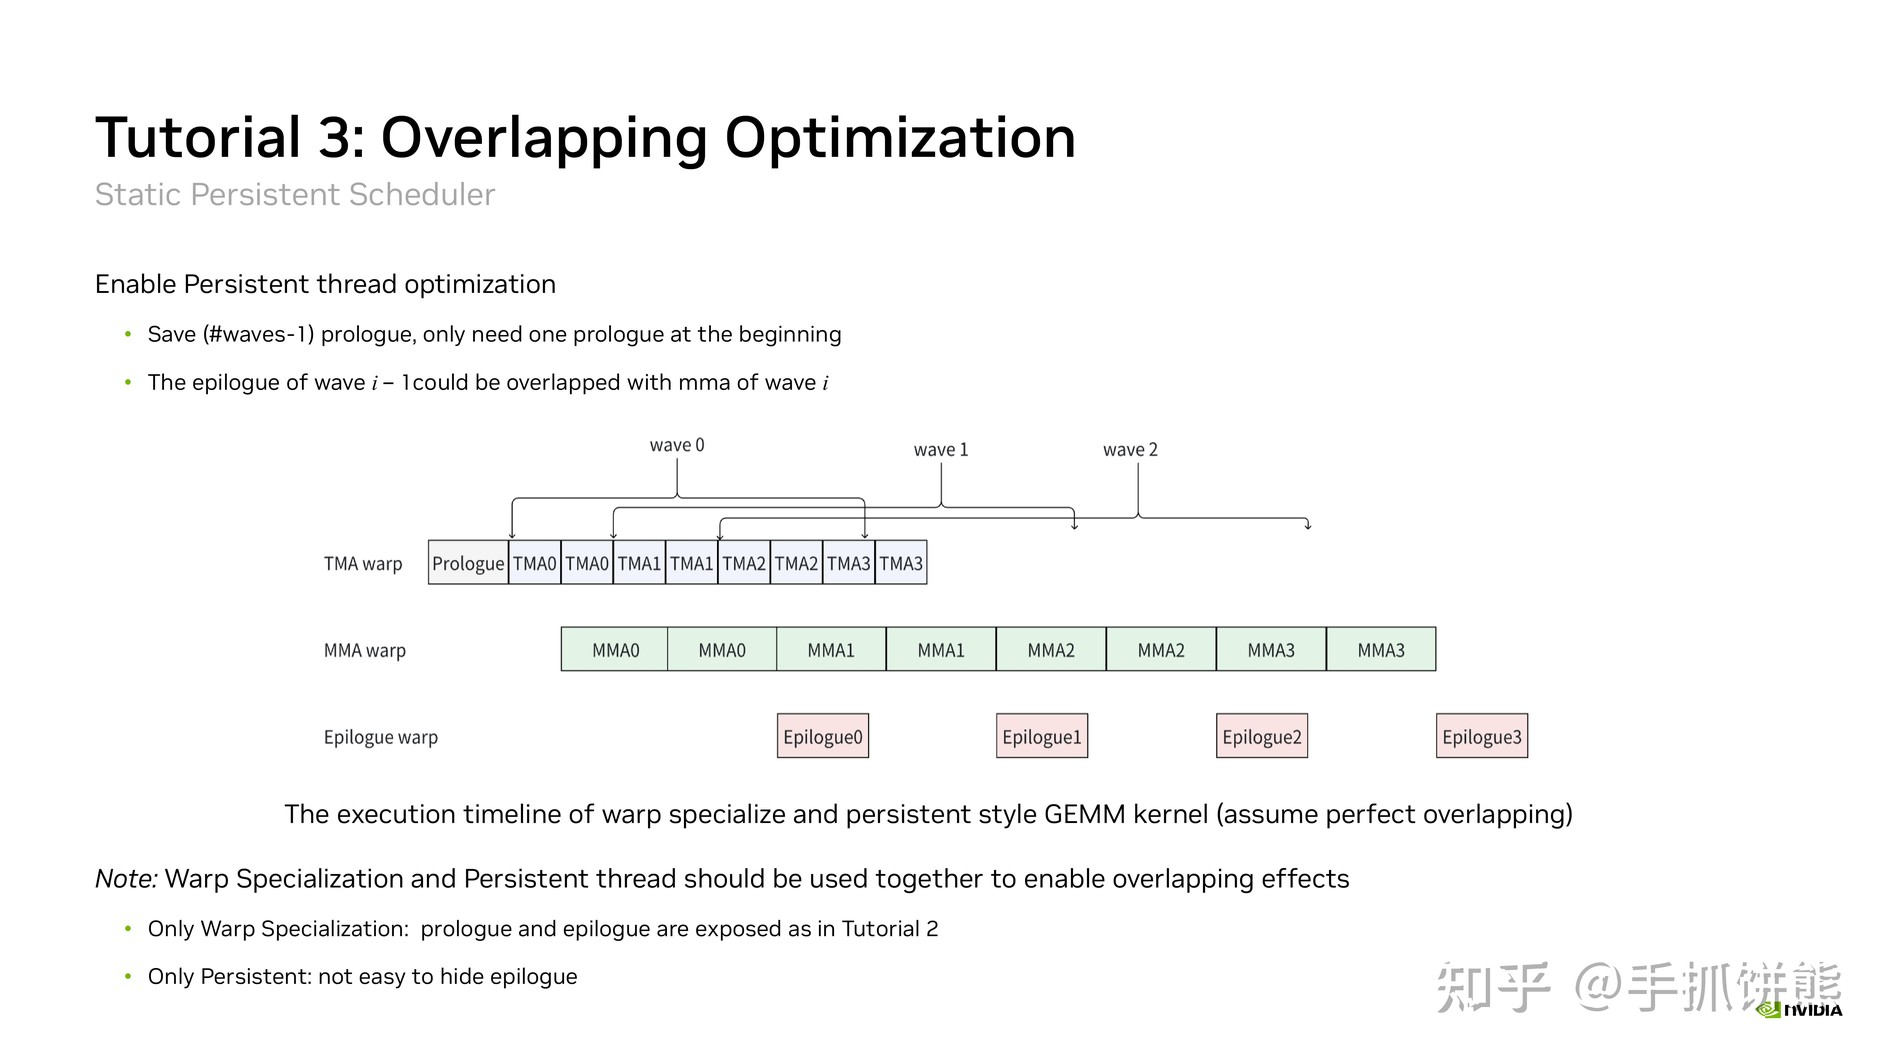
\includegraphics[width=0.9\textwidth]{figures/zhaoshangchun-03-cutlass-python/fig-22.jpg}
\end{figure}

\textbf{Persistent Kernel 的核心思想：}

让 CTA 一直驻留在 SM 上，处理完一个 tile 后直接处理下一个 tile，而不是退出后重新调度：

\begin{itemize}
\item \textbf{节省 (\#waves-1) 个 prologue：} 整个 kernel 只需要开始时的一次 prologue
\item \textbf{Wave i-1 的 epilogue 与 Wave i 的 MMA 重叠：} Warp Specialization 使得上一个 wave 的结果写回可以与下一个 wave 的计算同时进行
\end{itemize}

\textbf{关键约束：}

Warp Specialization 和 Persistent Kernel \textbf{必须配合使用}：

\begin{itemize}
\item \textbf{仅 Warp Specialization：} prologue 和 epilogue 仍然暴露（如 Tutorial 2）
\item \textbf{仅 Persistent：} epilogue 不容易隐藏
\item \textbf{两者结合：} 实现最大化重叠，如图中理想时间线所示
\end{itemize}

\textbf{理想执行时间线：} 只有第一个 wave 的 prologue 和最后一个 wave 的 epilogue 暴露，中间所有的 prologue 和 epilogue 都被计算所隐藏。

\subsection{3.13 Tutorial 3：NCU 验证}

\begin{figure}[H]\centering
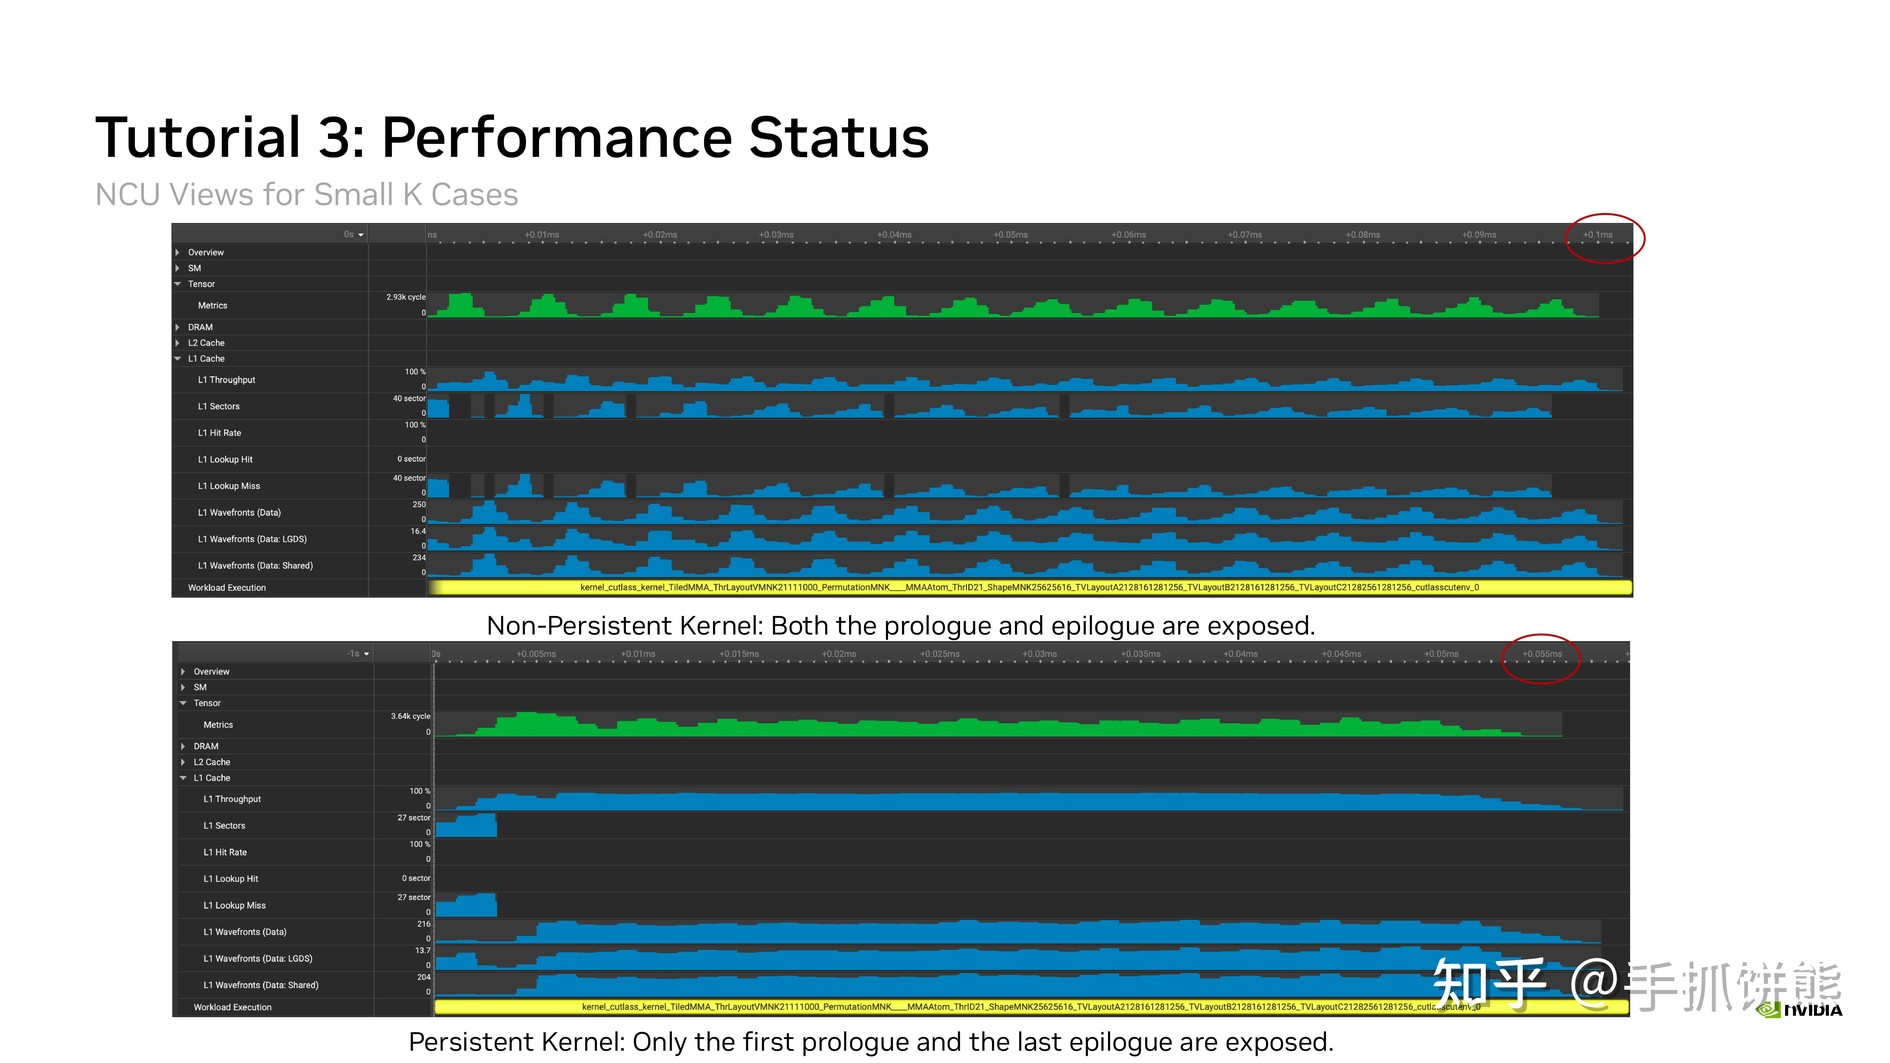
\includegraphics[width=0.9\textwidth]{figures/zhaoshangchun-03-cutlass-python/fig-23.jpg}
\end{figure}

\textbf{Nsight Compute 性能分析验证：}

通过 NCU 的时间线视图，可以清晰看到 Persistent Kernel 优化的效果：

\begin{itemize}
\item \textbf{Non-Persistent Kernel：} prologue 和 epilogue 都明确暴露在时间线中，每个 wave 都有明显的非计算开销
\item \textbf{Persistent Kernel：} 仅第一个 prologue 和最后一个 epilogue 暴露，中间部分计算连续进行
\end{itemize}

这从微架构层面验证了 Persistent Kernel 的优化效果。

\subsection{3.14 Tutorial 3：性能数据}

\begin{figure}[H]\centering
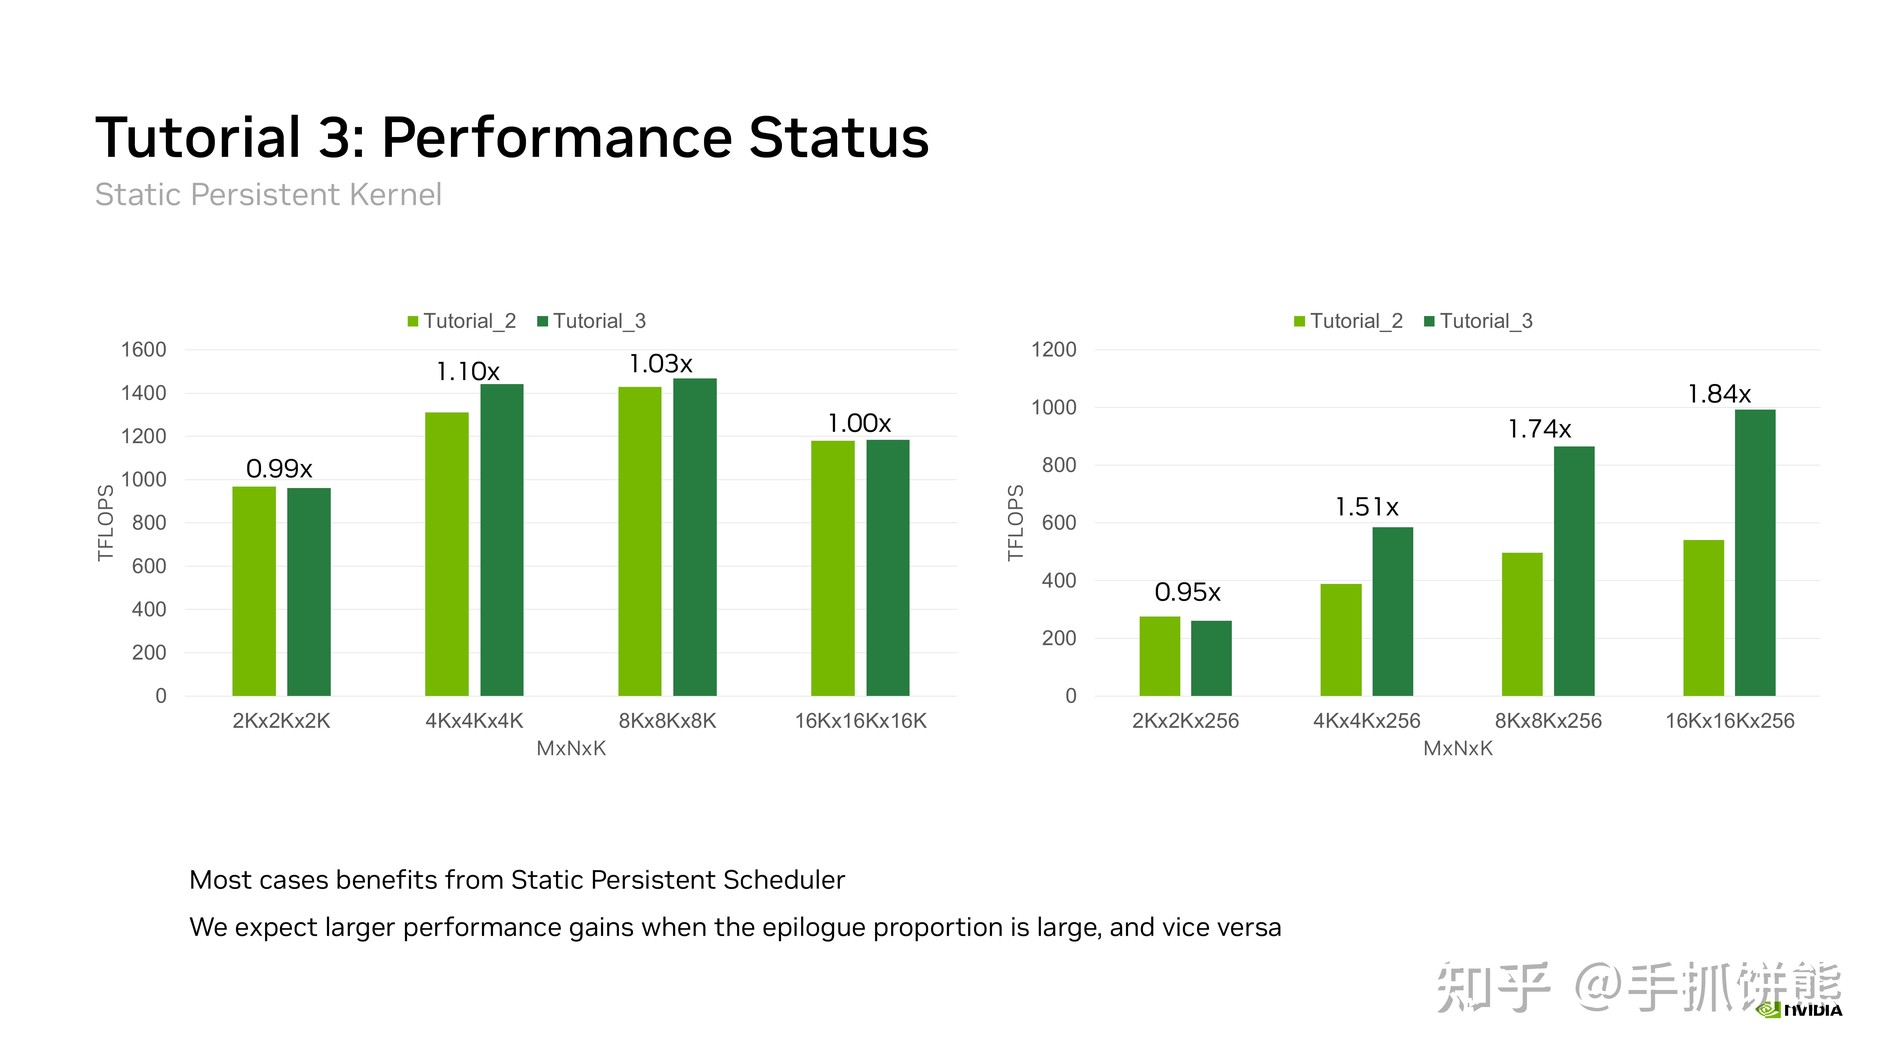
\includegraphics[width=0.9\textwidth]{figures/zhaoshangchun-03-cutlass-python/fig-24.jpg}
\end{figure}

\textbf{Static Persistent Scheduler 的性能收益：}

\textbf{大 K 场景（左图）：}

\begin{itemize}
\item 2\allowbreak{}K×2\allowbreak{}K×2\allowbreak{}K：0.99x（几乎不变）
\item 4\allowbreak{}K×4\allowbreak{}K×4\allowbreak{}K：1.10x
\item 8\allowbreak{}K×8\allowbreak{}K×8\allowbreak{}K：1.03x
\item 16\allowbreak{}K×16\allowbreak{}K×16\allowbreak{}K：1.00x
\end{itemize}

\textbf{小 K 场景（右图）：}

\begin{itemize}
\item 2\allowbreak{}K×2\allowbreak{}K×256：0.95x（略有下降，wave 数量不足以摊薄开销）
\item 4\allowbreak{}K×4\allowbreak{}K×256：1.51x
\item 8\allowbreak{}K×8\allowbreak{}K×256：1.74x
\item 16\allowbreak{}K×16\allowbreak{}K×256：\textbf{1.84x}
\end{itemize}

\textbf{性能规律：} Persistent Kernel 的收益与 epilogue 在总执行时间中的占比正相关。当 epilogue 占比大时（小 K），收益显著（最高 1.84x）；当 epilogue 占比小时（大 K），收益有限。

\subsection{3.15 Tutorial 4：Preferred 和 Fallback Clusters}

\begin{figure}[H]\centering
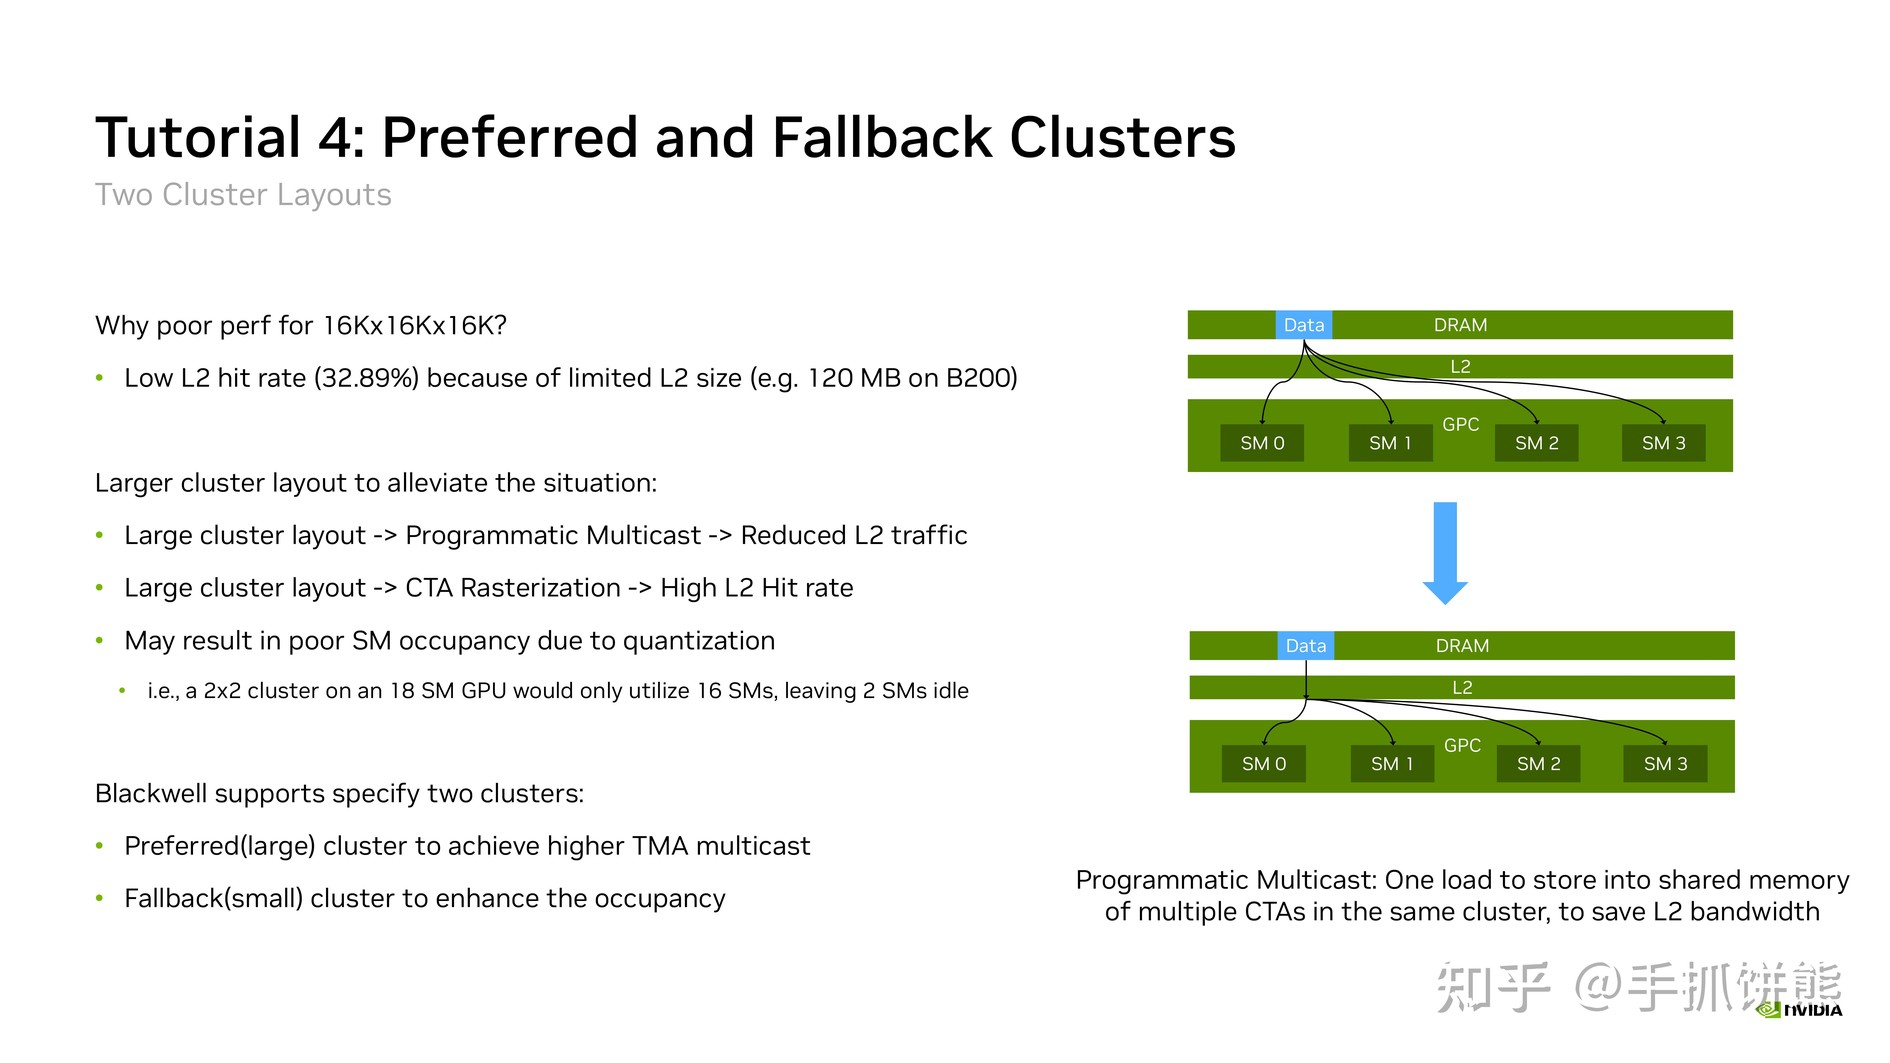
\includegraphics[width=0.9\textwidth]{figures/zhaoshangchun-03-cutlass-python/fig-25.jpg}
\end{figure}

\textbf{16\allowbreak{}K×16\allowbreak{}K×16\allowbreak{}K 性能瓶颈分析：}

为什么 Tutorial 3 在 16\allowbreak{}K×16\allowbreak{}K×16\allowbreak{}K 上没有收益？答案是 \textbf{L2 缓存命中率低}：

\begin{itemize}
\item B200 的 L2 缓存大小约为 120\allowbreak{}MB
\item 16\allowbreak{}K×16\allowbreak{}K×16\allowbreak{}K GEMM 的工作集远超 L2 容量
\item 导致 L2 命中率仅 \textbf{32.89\%}
\end{itemize}

\textbf{大 Cluster 的优势：} 使用更大的 cluster 布局可以缓解 L2 压力：

\begin{itemize}
\item \textbf{Programmatic Multicast：} 一次 TMA 加载可以将数据存入同一 cluster 内多个 CTA 的共享内存，如图中所示，一次加载 → 多个 SM 受益，大幅减少 L2 流量
\item \textbf{CTA Rasterization：} 大 cluster 布局配合 CTA 光栅化遍历顺序，提高 L2 命中率
\end{itemize}

\textbf{大 Cluster 的问题：}

量化效应（quantization）可能导致 SM 利用率不足：

\begin{itemize}
\item 例如，2×2 cluster 在 18 个 SM 的 GPU 上只能使用 16 个 SM，2 个 SM 空闲
\end{itemize}

\textbf{Blackwell 的解决方案——双 Cluster 策略：}

\begin{itemize}
\item \textbf{Preferred Cluster（大）：} 获得更高的 TMA multicast 收益
\item \textbf{Fallback Cluster（小）：} 在 preferred cluster 不满足对齐要求时使用，提升 SM 占用率
\end{itemize}

\subsection{3.16 Tutorial 4：性能结果}

\begin{figure}[H]\centering
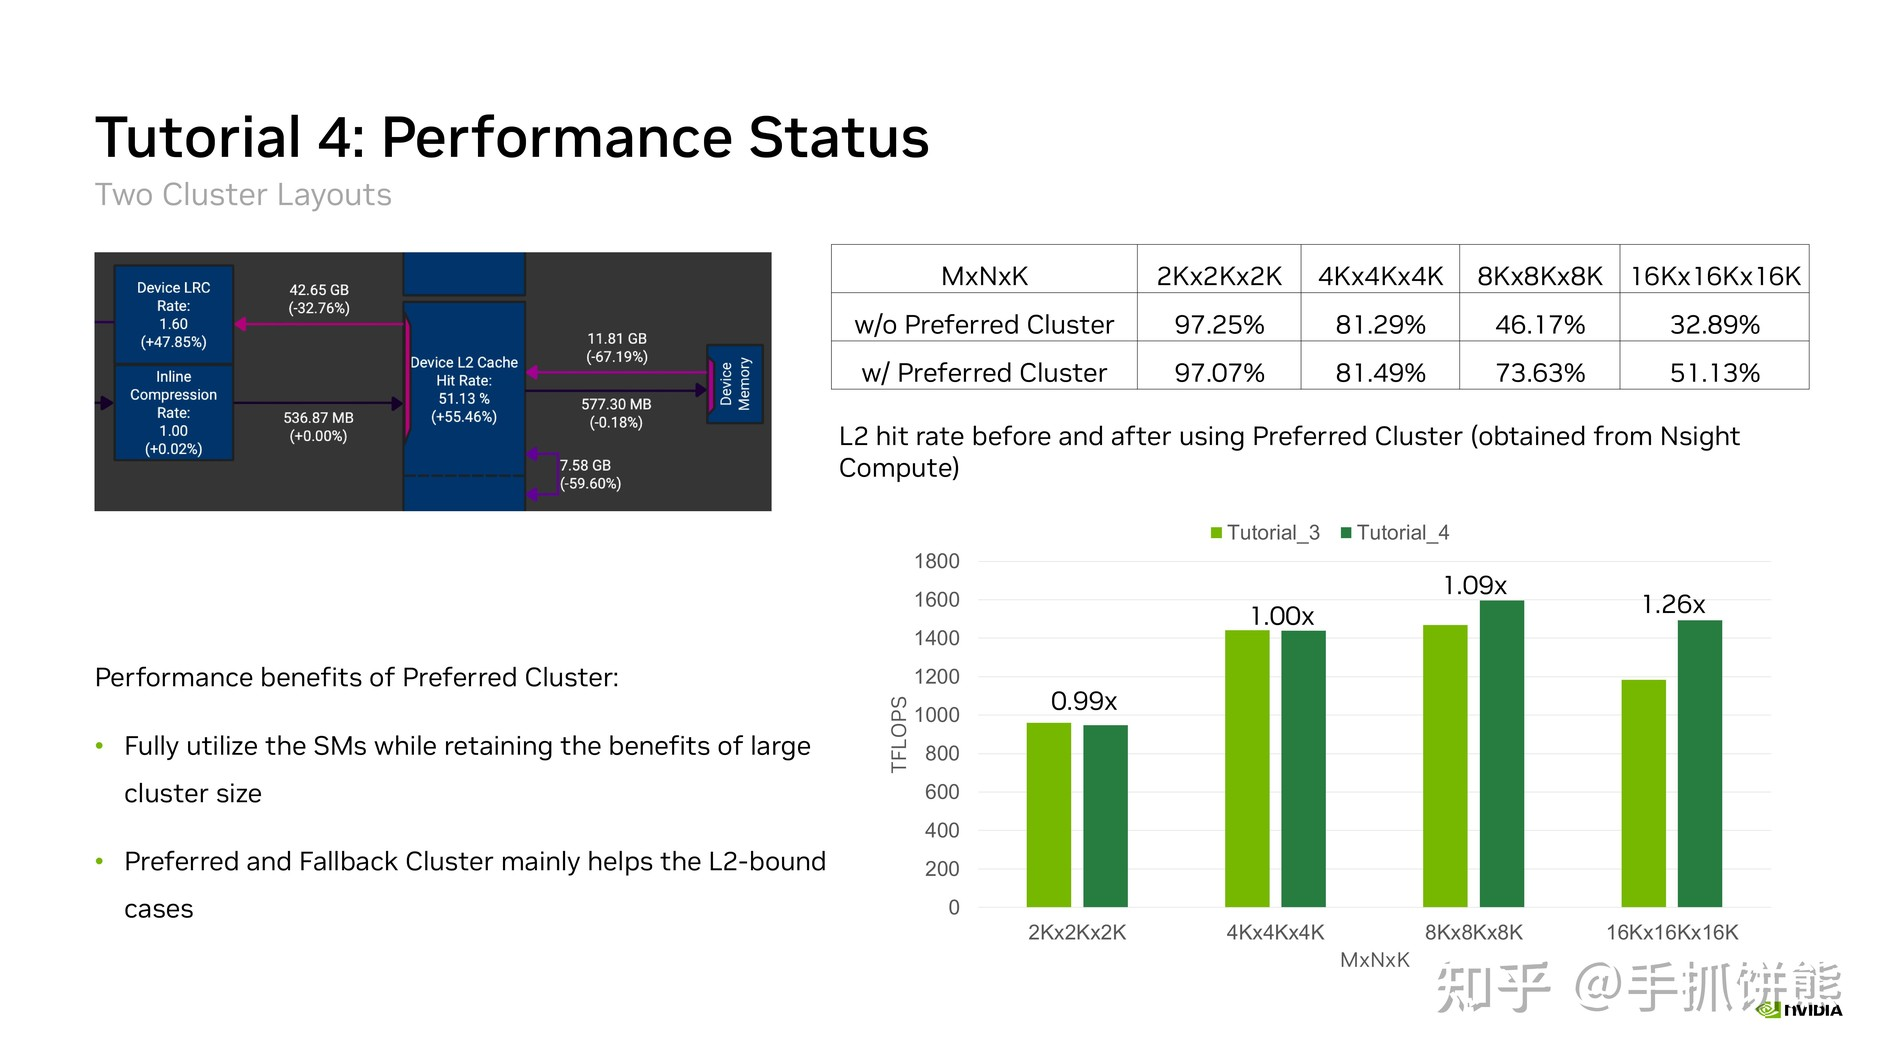
\includegraphics[width=0.9\textwidth]{figures/zhaoshangchun-03-cutlass-python/fig-26.jpg}
\end{figure}

\textbf{L2 命中率改善：}

\begin{table}[htbp]\centering\small
\begin{adjustbox}{max width=\textwidth}
\begin{tabular}{lll}
\toprule
Mx\allowbreak{}Nx\allowbreak{}K & 无 Preferred Cluster & 有 Preferred Cluster \\
\midrule
2\allowbreak{}K×2\allowbreak{}K×2\allowbreak{}K & 97.25\% & 97.07\% \\
4\allowbreak{}K×4\allowbreak{}K×4\allowbreak{}K & 81.29\% & 81.49\% \\
8\allowbreak{}K×8\allowbreak{}K×8\allowbreak{}K & 46.17\% & 73.63\% \\
16\allowbreak{}K×16\allowbreak{}K×16\allowbreak{}K & 32.89\% & 51.13\% \\
\bottomrule
\end{tabular}
\end{adjustbox}
\end{table}

\textbf{性能提升：}

\begin{itemize}
\item 2\allowbreak{}K×2\allowbreak{}K×2\allowbreak{}K：0.99x（L2 已经很高，无需优化）
\item 4\allowbreak{}K×4\allowbreak{}K×4\allowbreak{}K：1.00x
\item 8\allowbreak{}K×8\allowbreak{}K×8\allowbreak{}K：\textbf{1.09x}
\item 16\allowbreak{}K×16\allowbreak{}K×16\allowbreak{}K：\textbf{1.26x}
\end{itemize}

\textbf{关键结论：} Preferred/\allowbreak{}Fallback Clusters 优化主要针对 L2 缓存受限的大规模 GEMM 场景。8\allowbreak{}K 和 16\allowbreak{}K 的 L2 命中率分别从 46\%→74\% 和 33\%→51\%，性能提升显著。最终 16\allowbreak{}K 场景达到约 1597 TFLOPS。

\section{第四章：其他代表性优化场景}

本章讨论两个特殊但在实际生产中非常重要的优化场景。

\subsection{4.1 代表性场景概览}

\begin{figure}[H]\centering
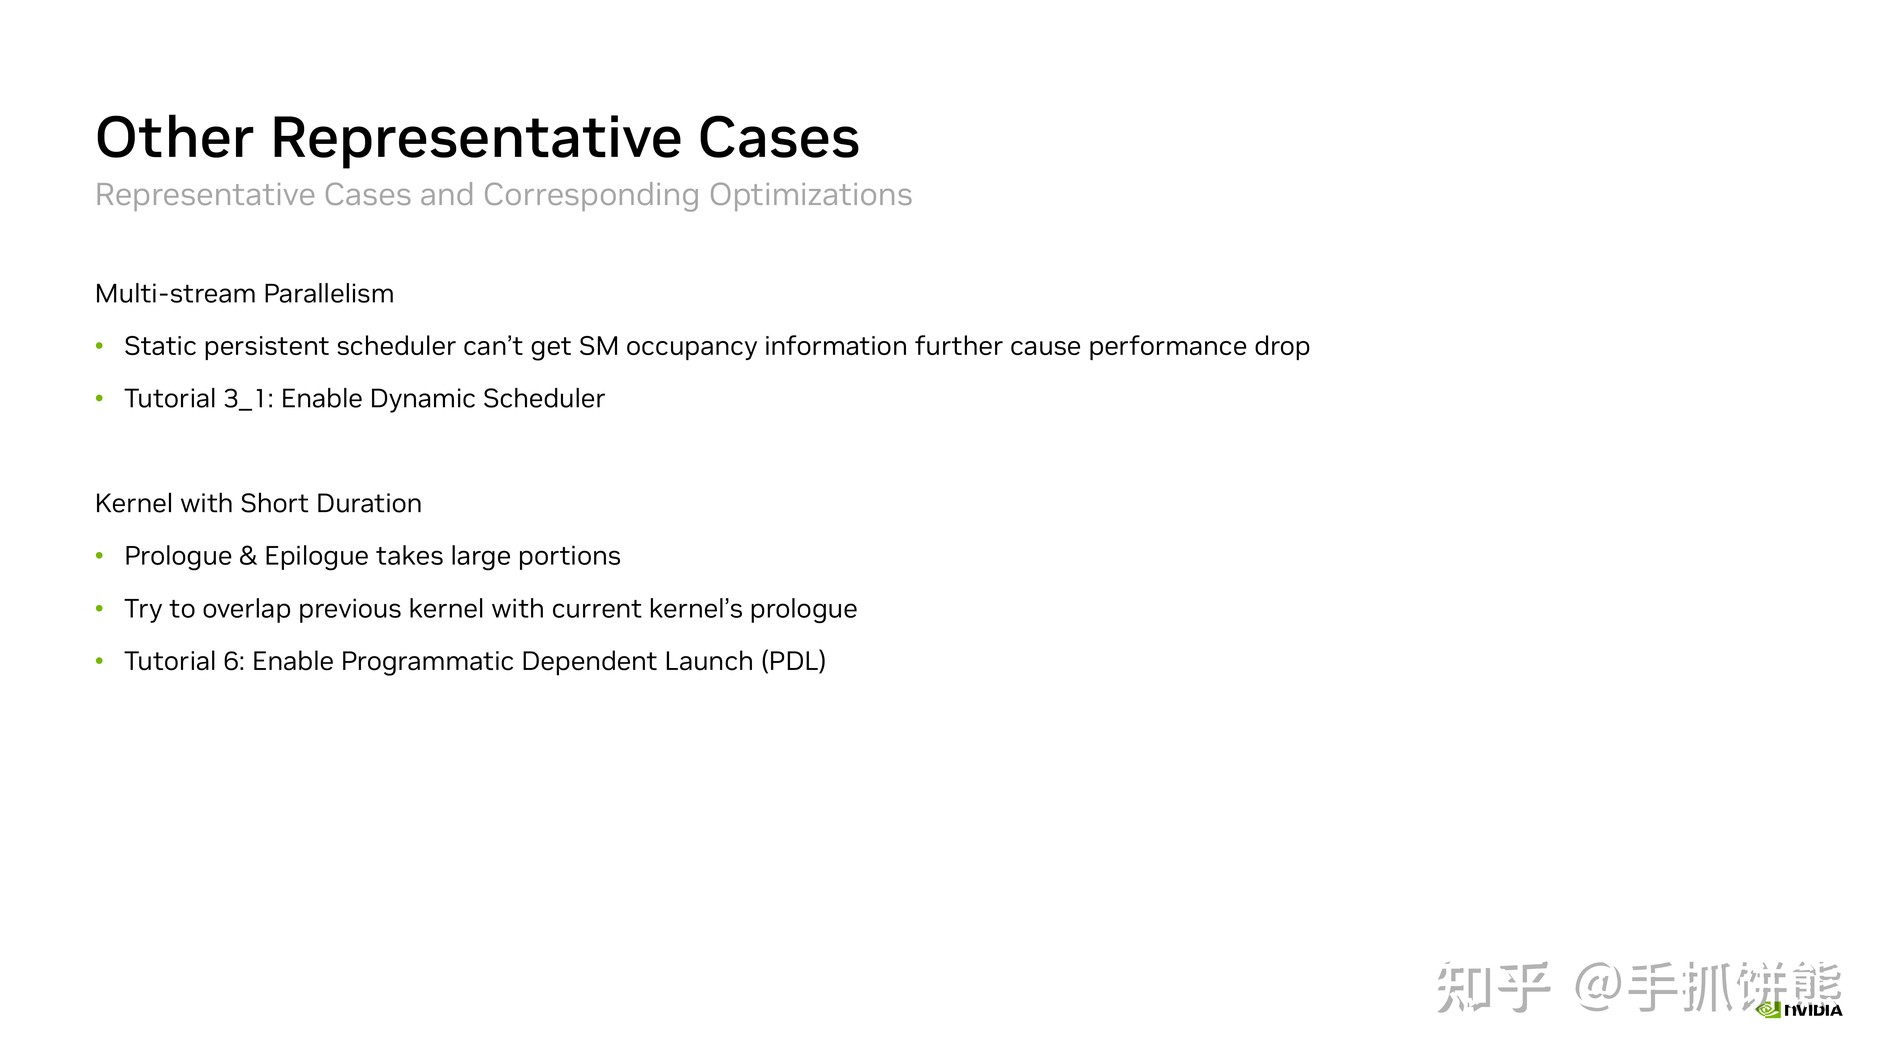
\includegraphics[width=0.9\textwidth]{figures/zhaoshangchun-03-cutlass-python/fig-27.jpg}
\end{figure}

\textbf{两大代表性场景：}

\textbf{场景 1 - 多流并行（Multi-stream Parallelism）：}

\begin{itemize}
\item 静态 Persistent Scheduler 无法获取 SM 占用信息，可能导致性能下降
\item 解决方案：Tutorial 3\_\allowbreak{}1 - 启用 \textbf{Dynamic Scheduler（CLC）}
\end{itemize}

\textbf{场景 2 - 短时 Kernel（Kernel with Short Duration）：}

\begin{itemize}
\item Prologue 和 Epilogue 占比过大
\item 解决方案：尝试将前一个 kernel 的 epilogue 与当前 kernel 的 prologue 重叠
\item Tutorial 6：启用 \textbf{Programmatic Dependent Launch（PDL）}
\end{itemize}

\subsection{4.2 Tutorial 3-1：Cluster Launch Control（CLC）}

\begin{figure}[H]\centering
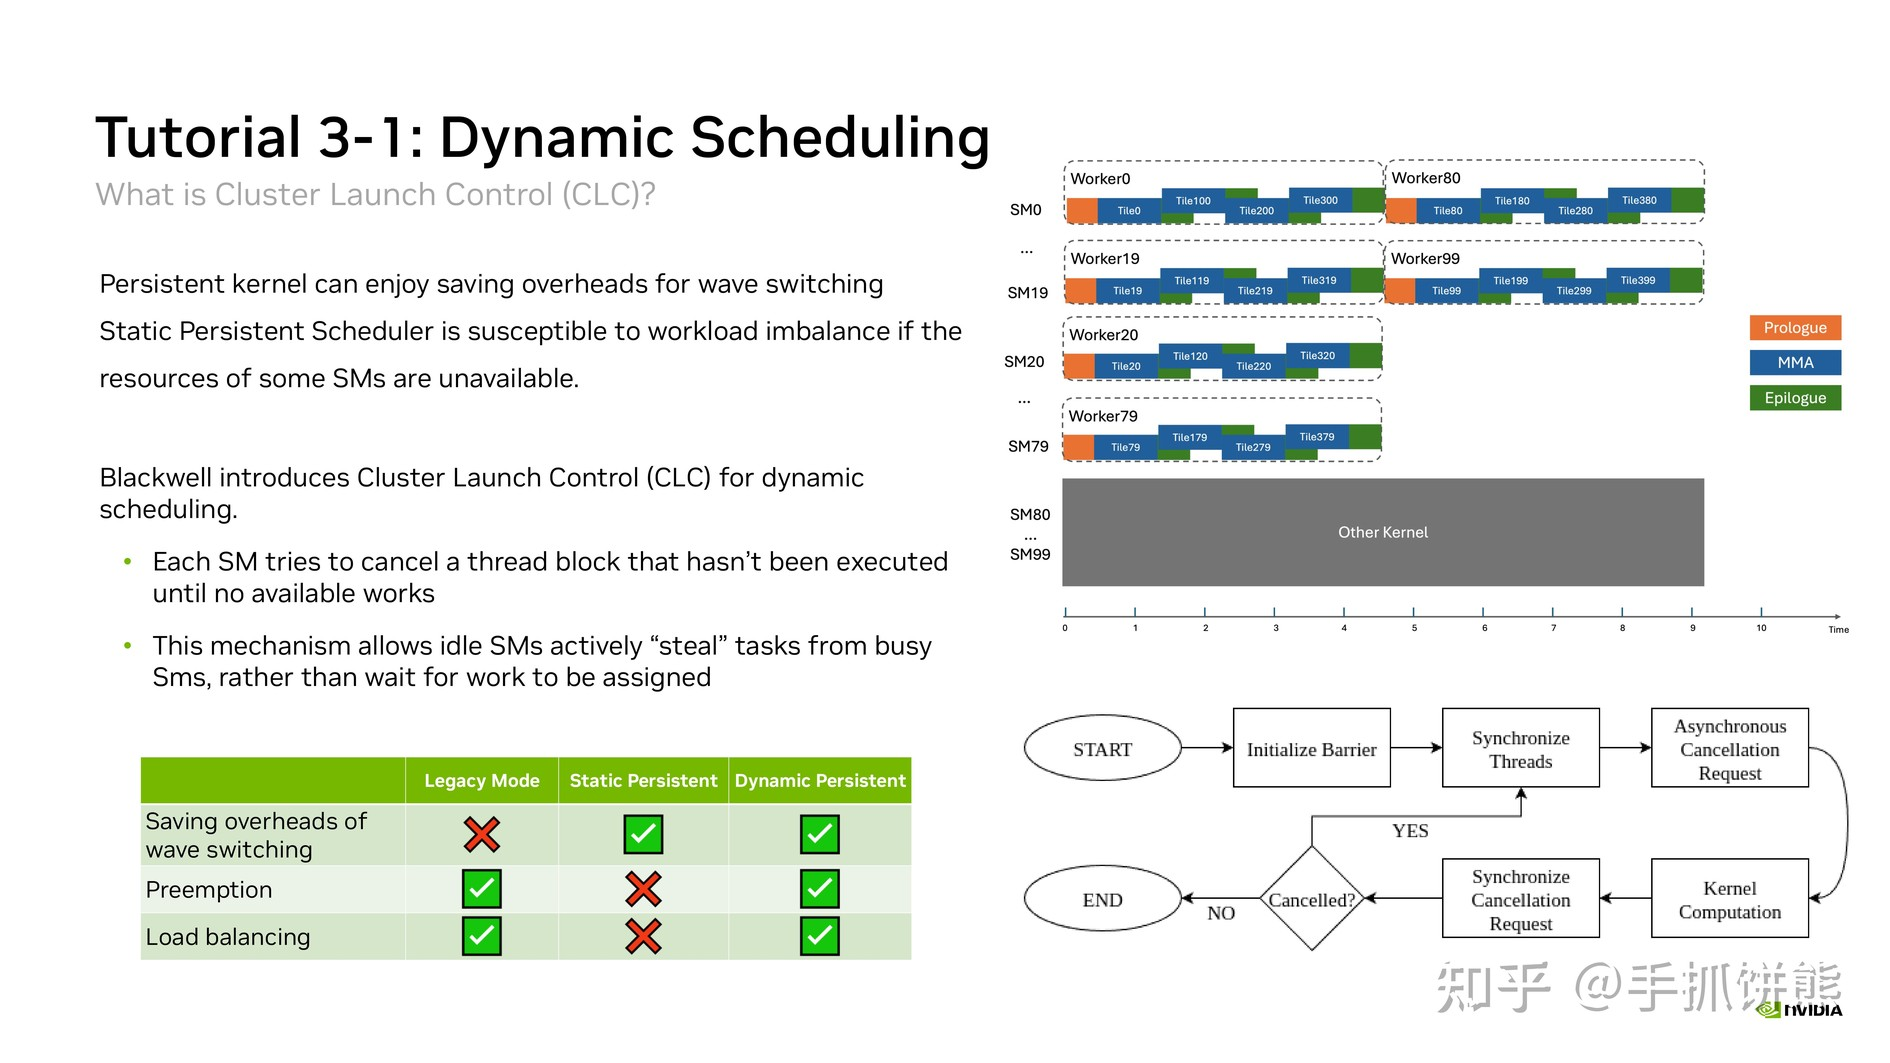
\includegraphics[width=0.9\textwidth]{figures/zhaoshangchun-03-cutlass-python/fig-28.jpg}
\end{figure}

\textbf{三种调度模式对比：}

\begin{table}[htbp]\centering\small
\begin{adjustbox}{max width=\textwidth}
\begin{tabular}{llll}
\toprule
特性 & Legacy Mode & Static Persistent & Dynamic Persistent \\
\midrule
节省波间切换开销 &  \ding{55}  &  \ding{51}  &  \ding{51}  \\
抢占（Preemption） &  \ding{55}  &  \ding{55}  &  \ding{51}  \\
负载均衡 &  \ding{55}  &  \ding{55}  &  \ding{51}  \\
\bottomrule
\end{tabular}
\end{adjustbox}
\end{table}

\textbf{CLC 的核心机制：}

Blackwell 引入的 \textbf{Cluster Launch Control（CLC）} 实现了动态调度：

\begin{itemize}
\item 每个 SM 尝试取消（cancel）尚未执行的 thread block，直到没有可用工作
\item 空闲 SM 可以主动 "窃取" 忙碌 SM 的任务（work stealing）
\item 相比 Static Persistent 的固定分配，CLC 能够更好地适应运行时的资源变化
\end{itemize}

\textbf{Static Persistent 的问题：}

Static Persistent Scheduler 在编译时就确定了 tile 到 SM 的映射。当部分 SM 资源不可用时（例如多流并行场景），会导致严重的负载不均衡。

\subsection{4.3 Tutorial 3-1：多流并行场景对比}

\begin{figure}[H]\centering
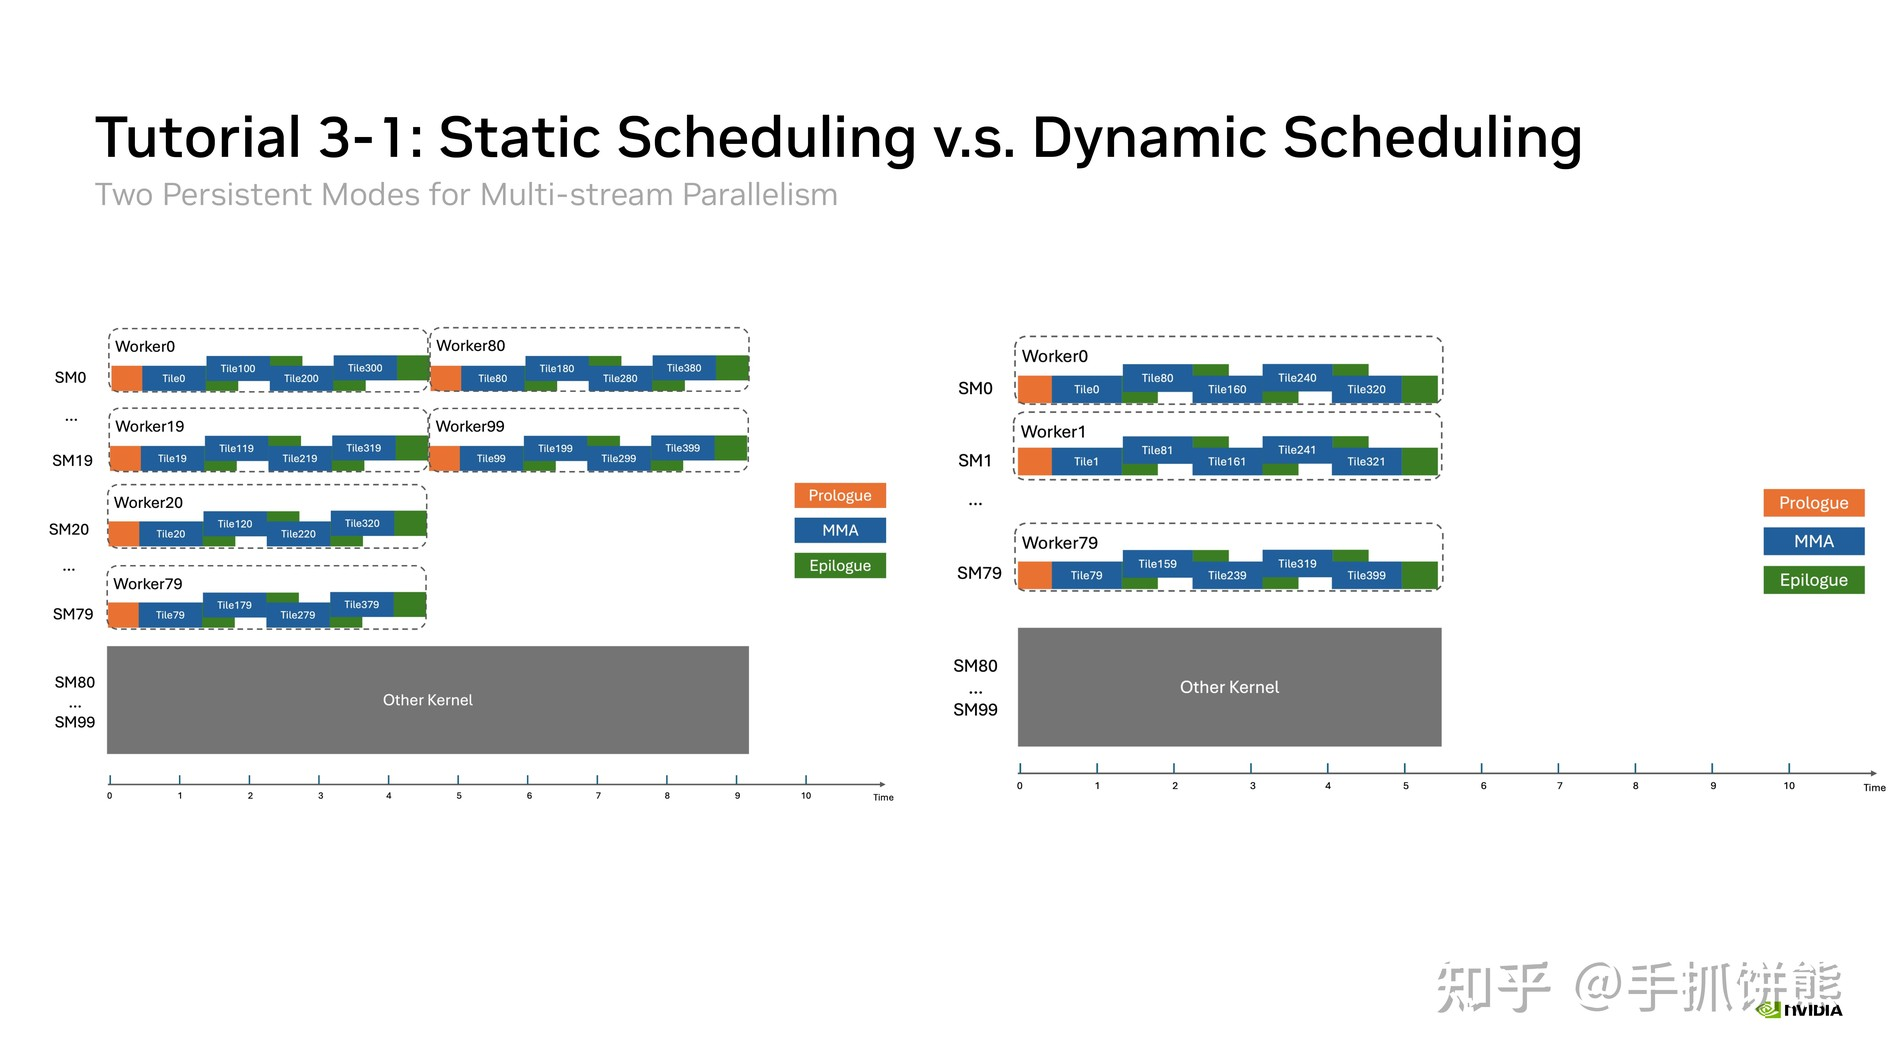
\includegraphics[width=0.9\textwidth]{figures/zhaoshangchun-03-cutlass-python/fig-29.jpg}
\end{figure}

该图展示了两种 Persistent 模式在多流并行场景下的行为差异：

\begin{itemize}
\item \textbf{Static Persistent：} tile 被静态分配到固定的 SM，当部分 SM 被其他 stream 的 kernel 占用时，分配到那些 SM 上的 tile 只能等待
\item \textbf{Dynamic Persistent：} 使用 CLC 动态分配，空闲 SM 可以立即获取新的 tile 执行，实现更好的负载均衡
\end{itemize}

\subsection{4.4 Tutorial 3-1：性能数据}

\begin{figure}[H]\centering
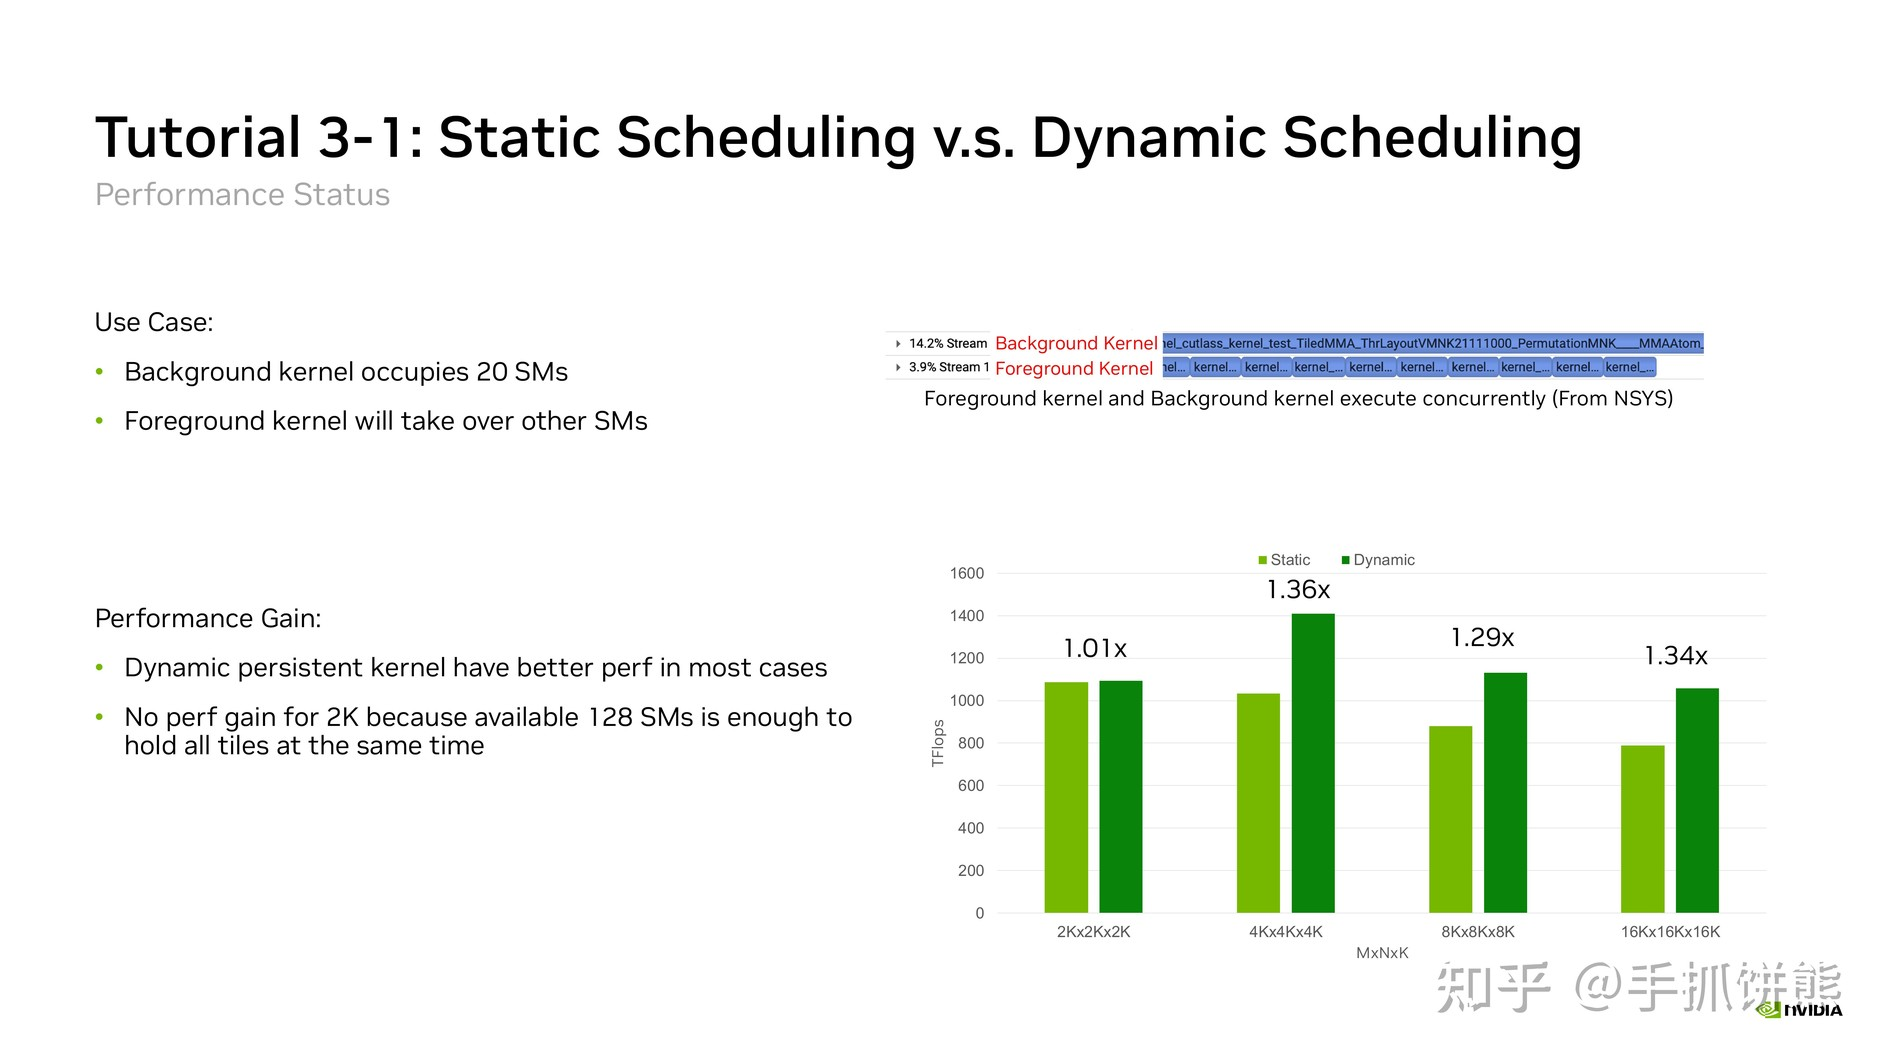
\includegraphics[width=0.9\textwidth]{figures/zhaoshangchun-03-cutlass-python/fig-30.jpg}
\end{figure}

\textbf{测试配置：}

\begin{itemize}
\item 背景 kernel（Background Kernel）占用 20 个 SM
\item 前台 kernel（Foreground Kernel）使用剩余的 SM
\end{itemize}

\textbf{从 NSYS 视图可以看到：} 前台 kernel 和背景 kernel 并发执行，前台 kernel 能够利用背景 kernel 未占用的 SM 资源。

\textbf{性能对比（Static vs Dynamic）：}

\begin{itemize}
\item 2\allowbreak{}K×2\allowbreak{}K×2\allowbreak{}K：1.01x（128 个可用 SM 足以同时容纳所有 tile，无需动态调度）
\item 4\allowbreak{}K×4\allowbreak{}K×4\allowbreak{}K：\textbf{1.36x}
\item 8\allowbreak{}K×8\allowbreak{}K×8\allowbreak{}K：\textbf{1.29x}
\item 16\allowbreak{}K×16\allowbreak{}K×16\allowbreak{}K：\textbf{1.34x}
\end{itemize}

\textbf{实践价值：} 在实际 LLM 推理中，多个 kernel 并发执行非常常见（例如通信与计算重叠）。Dynamic Persistent Scheduler 在这种场景下能够带来 1.3x 以上的性能提升，具有极高的实用价值。

\subsection{4.5 Tutorial 6：PDL 原理}

\begin{figure}[H]\centering
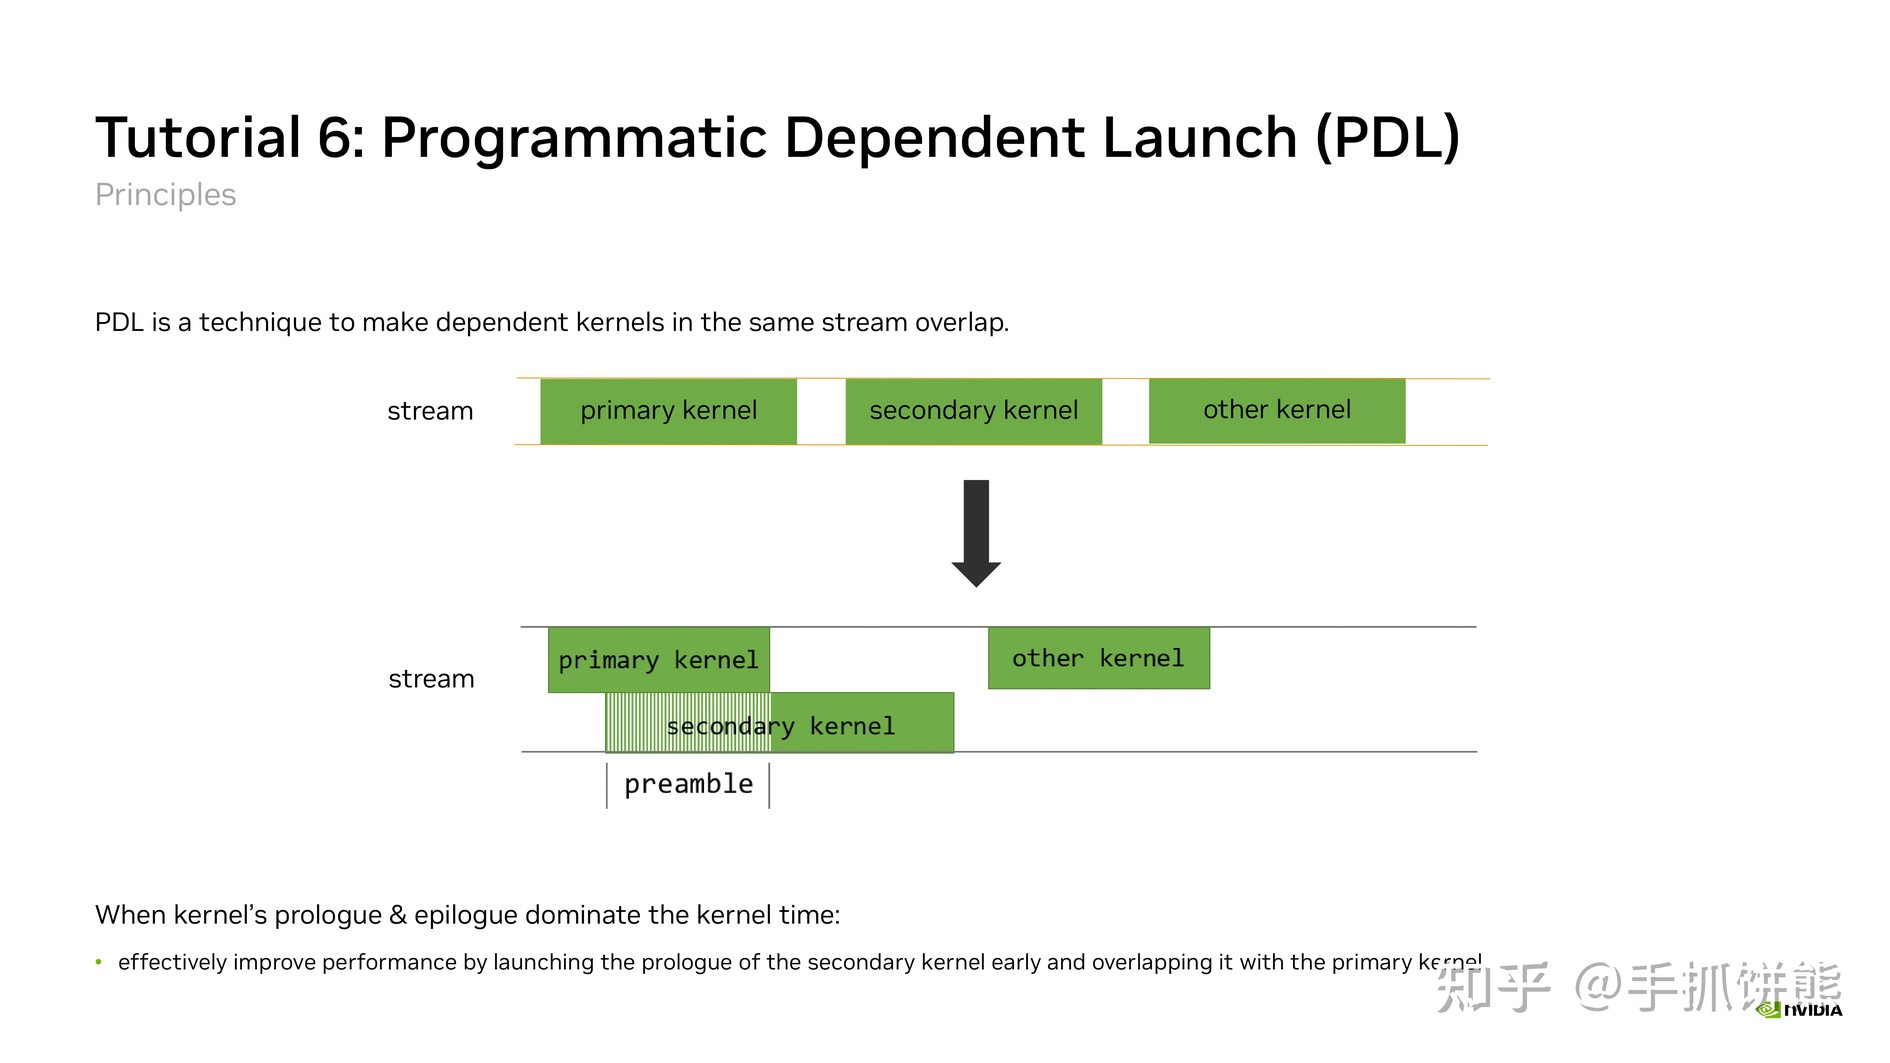
\includegraphics[width=0.9\textwidth]{figures/zhaoshangchun-03-cutlass-python/fig-31.jpg}
\end{figure}

\textbf{Programmatic Dependent Launch（PDL）的核心原理：}

PDL 是一种使同一 stream 中的依赖 kernel \textbf{实现重叠执行}的技术。

\textbf{适用场景：} 当 kernel 的 prologue 和 epilogue 主导执行时间时（即短时 kernel），通过提前启动次级 kernel 的 prologue 并与主 kernel 重叠，可以有效提升性能。

\textbf{执行模型（如图所示）：}

\begin{itemize}
\item \textbf{Without PDL：} primary kernel → secondary kernel → other kernel，串行执行
\item \textbf{With PDL：} primary kernel 的 epilogue 与 secondary kernel 的 prologue 重叠
\end{itemize}

传统 CUDA stream 语义要求同一 stream 内的 kernel 严格按序执行。PDL 打破了这一限制，允许在前一个 kernel 接近完成时就启动下一个 kernel 的初始化工作。

\subsection{4.6 Tutorial 6：PDL 实现}

\begin{figure}[H]\centering
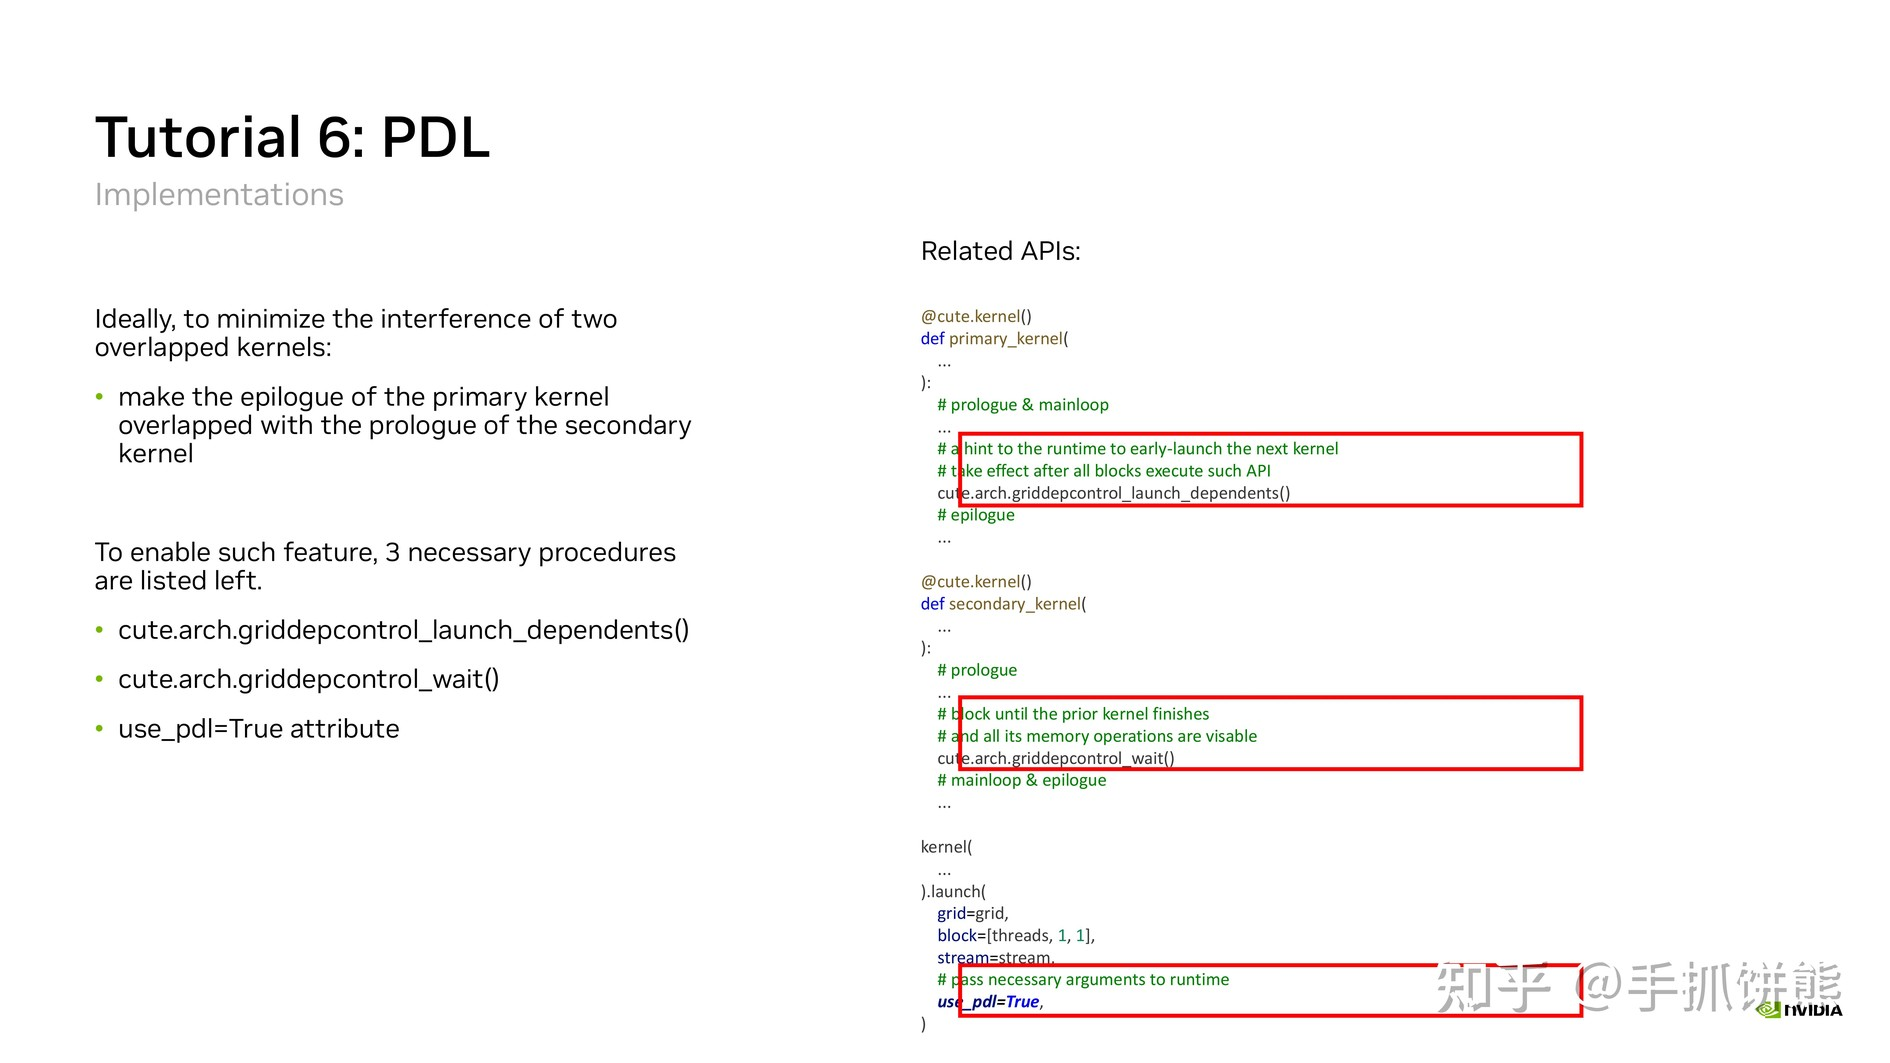
\includegraphics[width=0.9\textwidth]{figures/zhaoshangchun-03-cutlass-python/fig-32.jpg}
\end{figure}

\textbf{实现 PDL 需要 3 个关键步骤：}

\textbf{Step 1 - Primary Kernel 中声明可以启动后续 kernel：}

\begin{lstlisting}
@cute.kernel()
def primary_kernel(...):
    # prologue & mainloop
    ...
    # 告知 runtime 可以提前启动下一个 kernel
    cute.arch.griddepcontrol_launch_dependents()
    # epilogue
    ...
\end{lstlisting}

\texttt{g\allowbreak{}r\allowbreak{}i\allowbreak{}d\allowbreak{}d\allowbreak{}e\allowbreak{}p\allowbreak{}c\allowbreak{}o\allowbreak{}n\allowbreak{}t\allowbreak{}r\allowbreak{}o\allowbreak{}l\allowbreak{}\_\allowbreak{}l\allowbreak{}a\allowbreak{}u\allowbreak{}n\allowbreak{}c\allowbreak{}h\allowbreak{}\_\allowbreak{}d\allowbreak{}e\allowbreak{}p\allowbreak{}e\allowbreak{}n\allowbreak{}d\allowbreak{}e\allowbreak{}n\allowbreak{}t\allowbreak{}s\allowbreak{}(\allowbreak{})} 是一个\textbf{集体操作}——当所有 block 都执行到这个 API 时，runtime 才会实际启动下一个 kernel。

\textbf{Step 2 - Secondary Kernel 中等待前序 kernel 完成：}

\begin{lstlisting}
@cute.kernel()
def secondary_kernel(...):
    # prologue
    ...
    # 等待前序 kernel 完成且内存操作可见
    cute.arch.griddepcontrol_wait()
    # mainloop & epilogue
    ...
\end{lstlisting}

\texttt{griddepcontrol\_\allowbreak{}wait()} 确保了数据一致性——secondary kernel 的 mainloop 不会在 primary kernel 的内存操作完全可见之前开始。

\textbf{Step 3 - Launch 时启用 PDL：}

\begin{lstlisting}
kernel(...).launch(
    grid=grid,
    block=[threads, 1, 1],
    stream=stream,
    use_pdl=True,  # 关键参数
)
\end{lstlisting}

\subsection{4.7 Tutorial 6：PDL 应用设计}

\begin{figure}[H]\centering
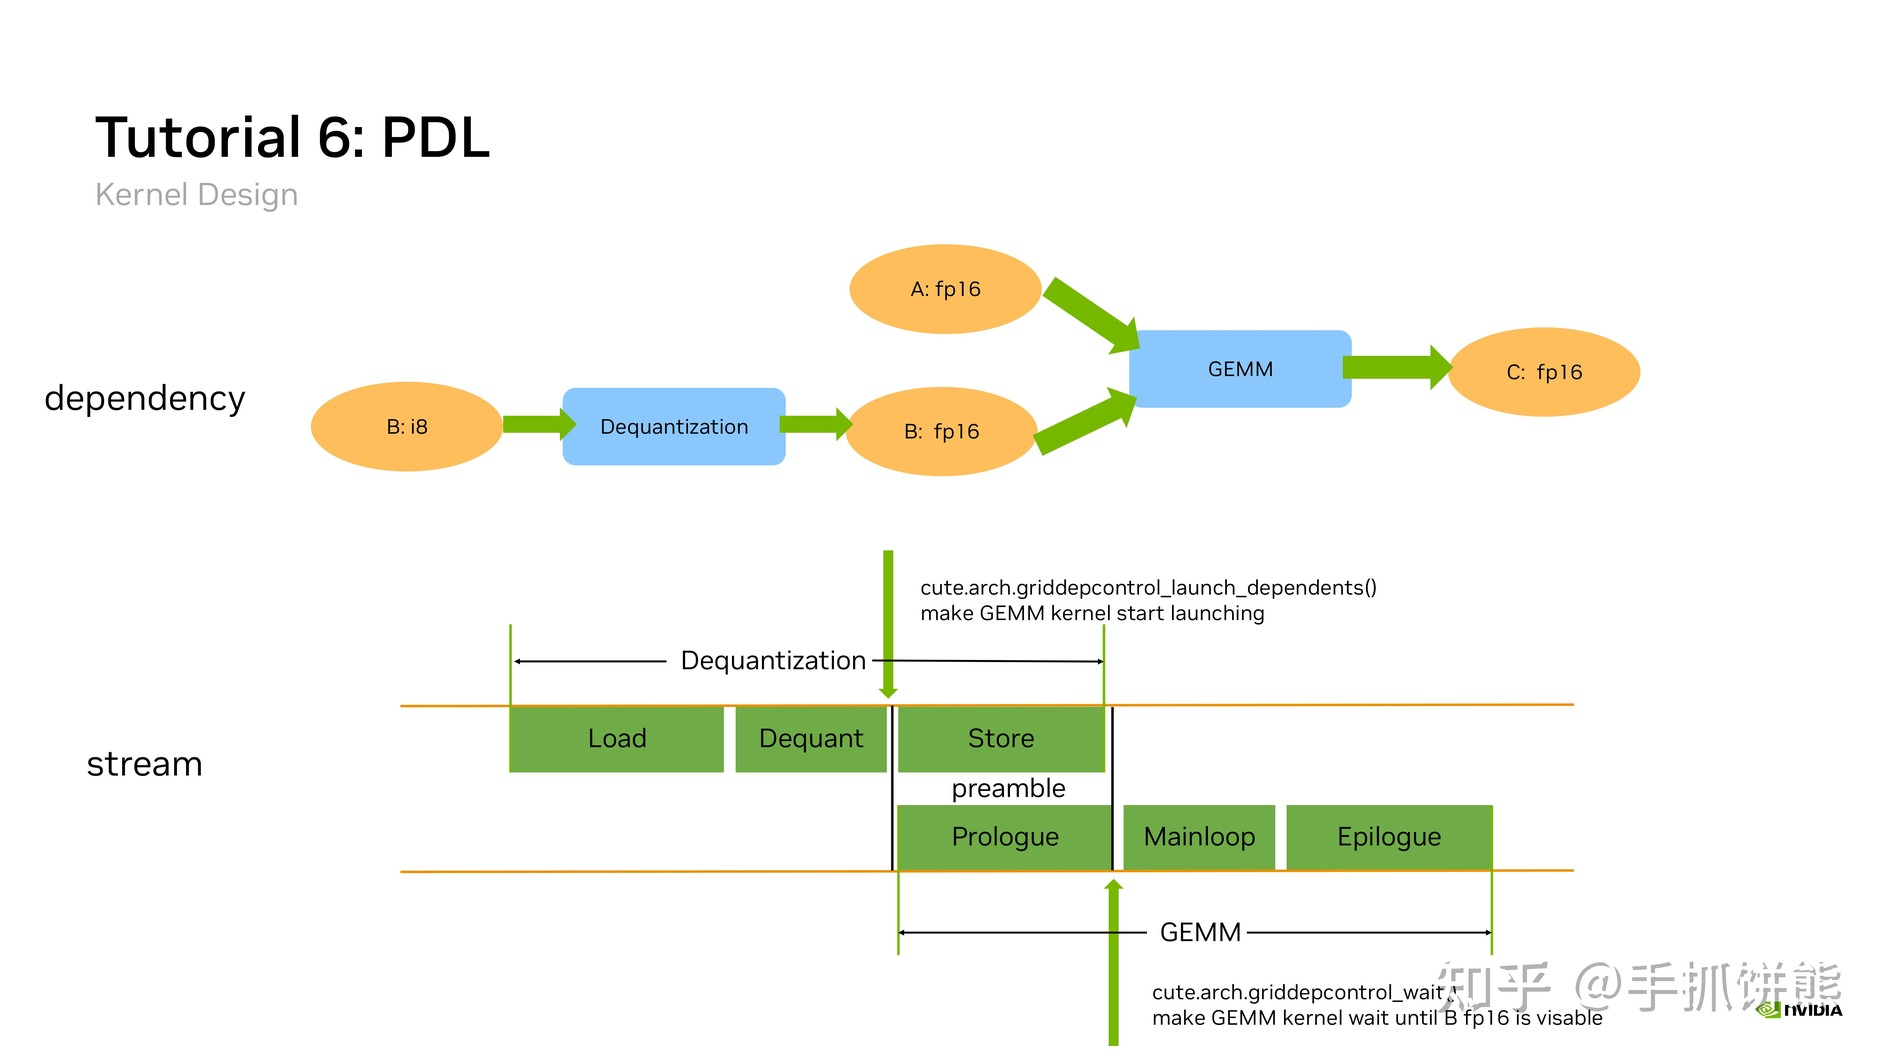
\includegraphics[width=0.9\textwidth]{figures/zhaoshangchun-03-cutlass-python/fig-33.jpg}
\end{figure}

\textbf{实际应用案例：Dequantization + GEMM}

本 Tutorial 设计了一个实际的 PDL 应用场景：

\textbf{两个 Kernel 的流水线：}

\begin{enumerate}
\item \textbf{Dequantization Kernel（Primary）：}
\item Prologue：加载量化的 B 矩阵（i8 格式）
\item Mainloop：执行反量化操作
\item Epilogue：将 fp16 格式的 B 矩阵写回 + 调用 \texttt{g\allowbreak{}r\allowbreak{}i\allowbreak{}d\allowbreak{}d\allowbreak{}e\allowbreak{}p\allowbreak{}c\allowbreak{}o\allowbreak{}n\allowbreak{}t\allowbreak{}r\allowbreak{}o\allowbreak{}l\allowbreak{}\_\allowbreak{}l\allowbreak{}a\allowbreak{}u\allowbreak{}n\allowbreak{}c\allowbreak{}h\allowbreak{}\_\allowbreak{}d\allowbreak{}e\allowbreak{}p\allowbreak{}e\allowbreak{}n\allowbreak{}d\allowbreak{}e\allowbreak{}n\allowbreak{}t\allowbreak{}s\allowbreak{}(\allowbreak{})}
\item \textbf{GEMM Kernel（Secondary）：}
\item Preamble/\allowbreak{}Prologue：预加载 A 矩阵等准备工作
\item Dependency：调用 \texttt{griddepcontrol\_\allowbreak{}wait()} 等待 fp16 B 可见
\item Mainloop + Epilogue：执行标准 GEMM
\end{enumerate}

\textbf{重叠效果：}

\begin{itemize}
\item GEMM Kernel 的 prologue（加载 A 矩阵、初始化）与 Dequantization Kernel 的最后阶段重叠
\item 整体端到端延迟 = Dequant 全部 + GEMM 除去 prologue 的部分
\end{itemize}

\subsection{4.8 Tutorial 6：PDL 性能}

\begin{figure}[H]\centering
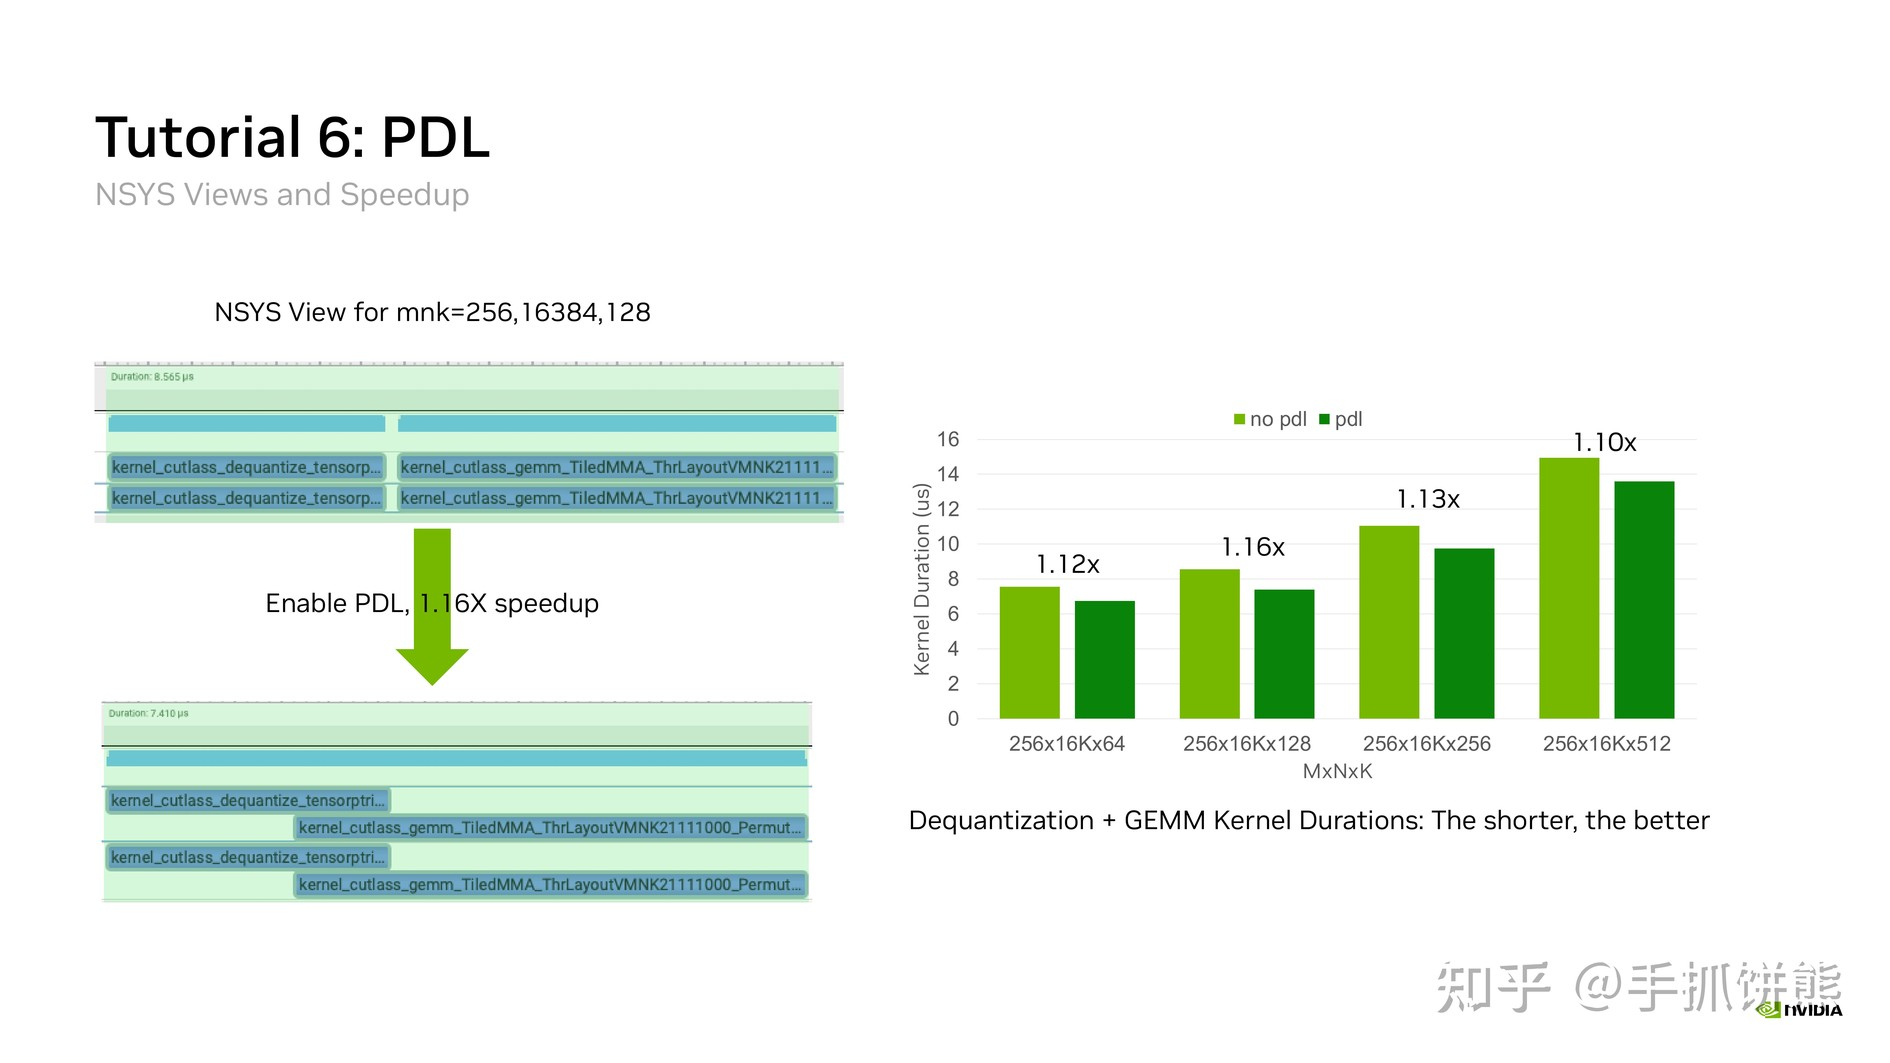
\includegraphics[width=0.9\textwidth]{figures/zhaoshangchun-03-cutlass-python/fig-34.jpg}
\end{figure}

\textbf{NSYS 视图验证：}

从 NSYS 的时间线视图中，在 mnk=256×16384×128 的场景下，可以清楚看到两个 kernel 的重叠执行。

\textbf{性能数据（Dequantization + GEMM 总时间）：}

\begin{itemize}
\item 256×16\allowbreak{}K×64：\textbf{1.12x} speedup
\item 256×16\allowbreak{}K×128：\textbf{1.16x} speedup
\item 256×16\allowbreak{}K×256：\textbf{1.13x} speedup
\item 256×16\allowbreak{}K×512：\textbf{1.10x} speedup
\end{itemize}

\textbf{适用场景分析：} PDL 在以下条件下效果最佳：(1) Kernel 执行时间短；(2) Prologue 占比较大；(3) 有明确的数据依赖关系。在 LLM 推理中，量化推理场景下的 Dequant+GEMM 正是典型应用。

\section{第五章：总结}

\subsection{5.1 优化技术全景总结}

\begin{figure}[H]\centering
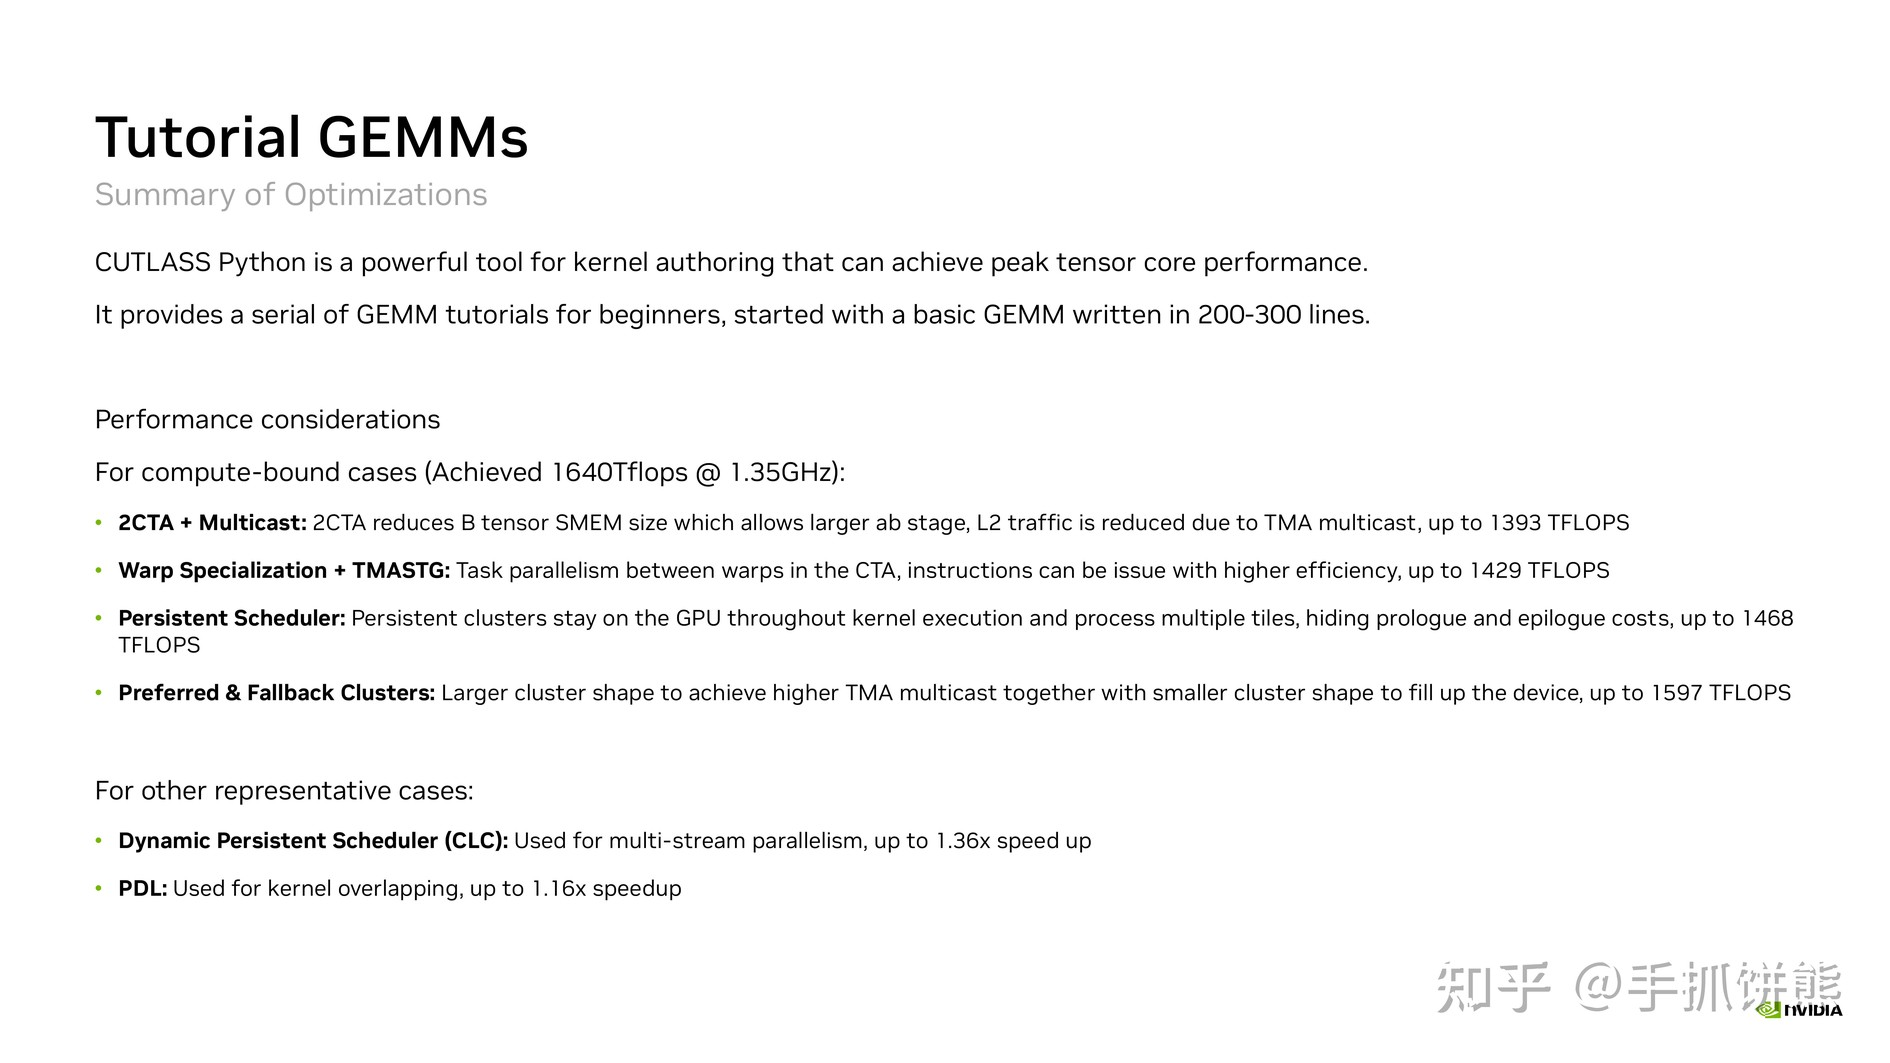
\includegraphics[width=0.9\textwidth]{figures/zhaoshangchun-03-cutlass-python/fig-35.jpg}
\end{figure}

\textbf{CUTLASS Python 的定位：}

CUTLASS Python 是一个强大的 kernel 编写工具，能够达到峰值 Tensor Core 性能。它提供了一系列面向初学者的 GEMM 教程，从一个仅需 200-300 行的基础 GEMM 开始逐步深入。

\textbf{计算密集型场景优化总结（基线：1640 TFLOPS @ 1.35\allowbreak{}GHz）：}

\begin{table}[htbp]\centering\small
\begin{adjustbox}{max width=\textwidth}
\begin{tabular}{lll}
\toprule
优化技术 & 原理 & 达到 TFLOPS \\
\midrule
2\allowbreak{}CTA + Multicast & 2\allowbreak{}CTA 减少 B tensor SMEM 大小以允许更大的 ab stage；TMA multicast 减少 L2 流量 & 1393 \\
Warp Specialization + TMA STG & CTA 内 warp 间任务并行；指令可以更高效地发射 & 1429 \\
Persistent Scheduler & Persistent cluster 在 kernel 执行期间驻留 GPU，处理多个 tile，隐藏 prologue/\allowbreak{}epilogue 开销 & 1468 \\
Preferred \& Fallback Clusters & 大 cluster 获得更高 TMA multicast + 小 cluster 填充设备 & 1597 \\
\bottomrule
\end{tabular}
\end{adjustbox}
\end{table}

\textbf{其他代表性场景：}

\begin{itemize}
\item \textbf{Dynamic Persistent Scheduler（CLC）：} 用于多流并行，最高 \textbf{1.36x} 加速
\item \textbf{PDL：} 用于 kernel 重叠执行，最高 \textbf{1.16x} 加速
\end{itemize}

\subsection{5.2 技术演进全景}

\begin{figure}[H]\centering
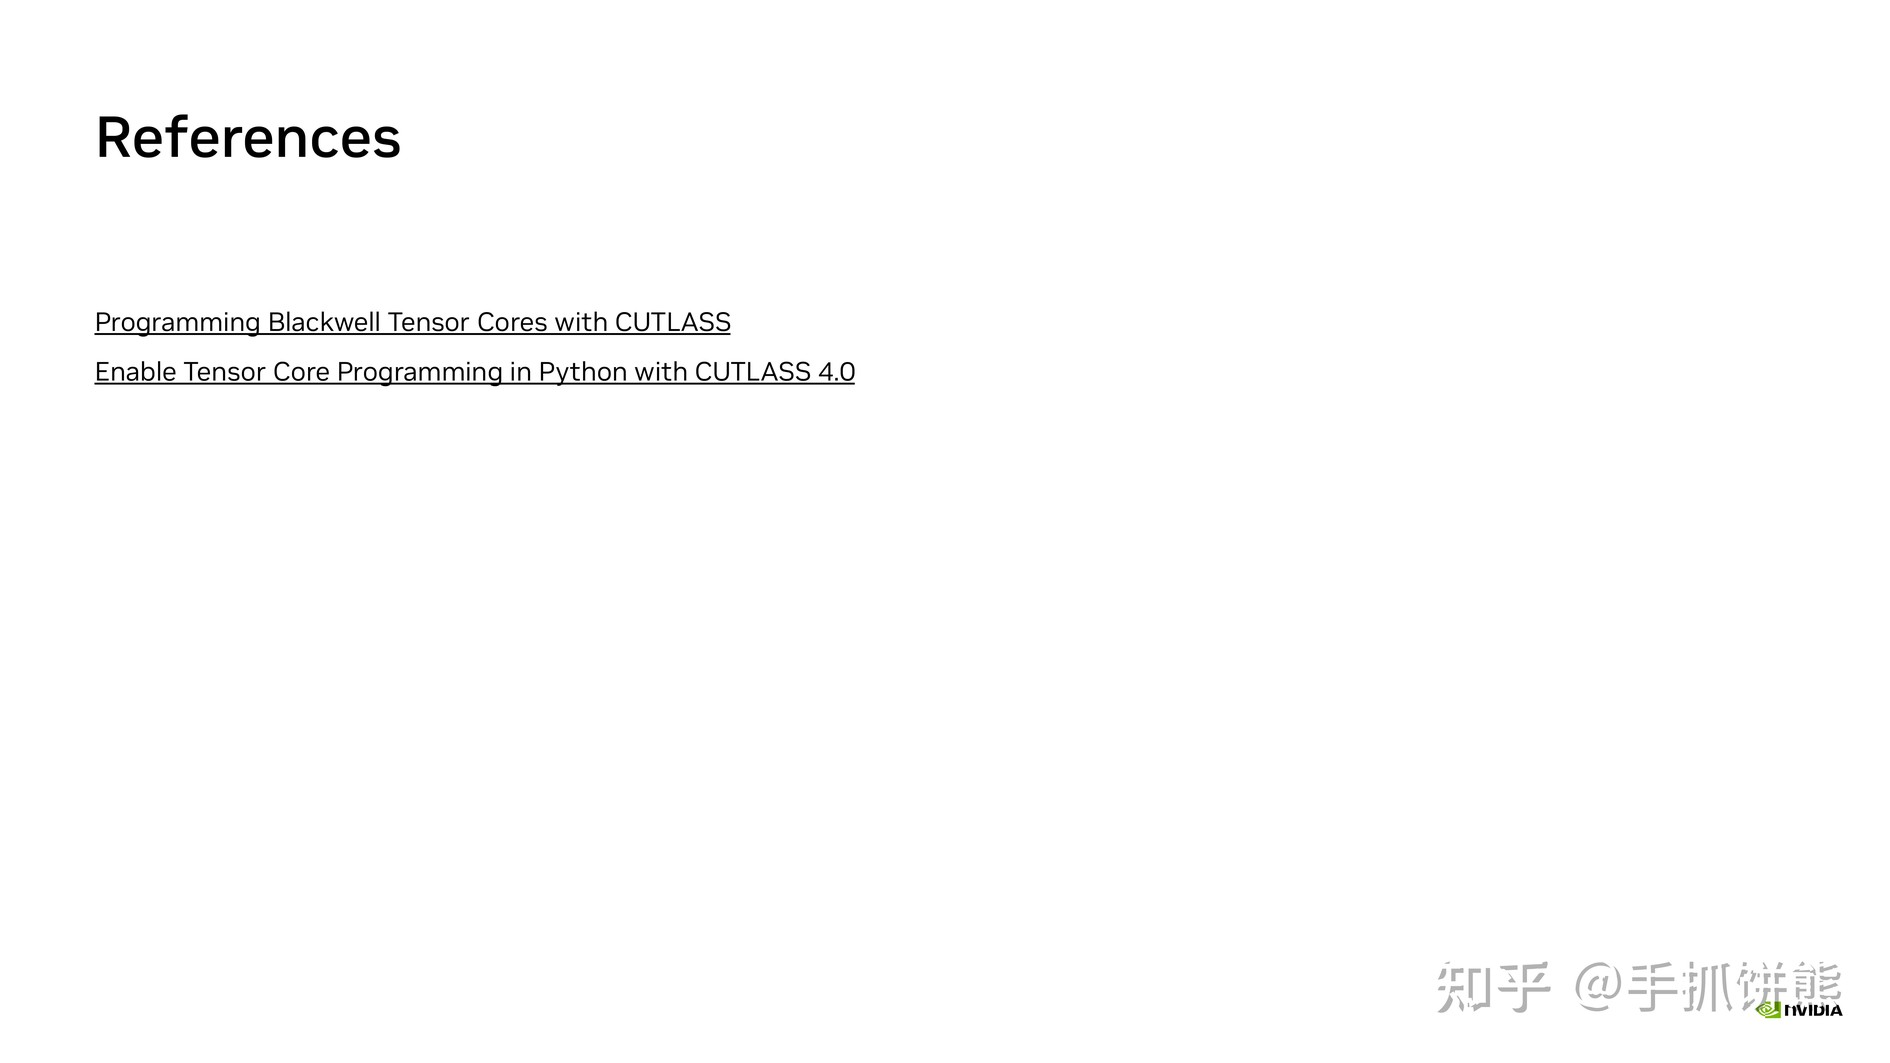
\includegraphics[width=0.9\textwidth]{figures/zhaoshangchun-03-cutlass-python/fig-36.jpg}
\end{figure}

\textbf{推荐参考资源：}

\begin{itemize}
\item "Programming Blackwell Tensor Cores with CUTLASS" - 深入 Blackwell Tensor Core 编程
\item "Enable Tensor Core Programming in Python with CUTLASS 4.0" - CUTLASS 4.0 Python 接口详解
\end{itemize}

这些资源提供了更深层次的技术细节，建议有兴趣的读者进一步阅读。

\endgroup
